\documentclass[12pt]{report}

% Paquetes LaTeX y estilos globales
\usepackage[utf8]{inputenc}
\usepackage{multicol}
\usepackage{xcolor}
\usepackage{subfigure}
\usepackage[spanish,es-tabla]{babel}
\usepackage[utf8]{inputenc}
\usepackage{graphicx}
\usepackage{titlesec}
\usepackage[bookmarks,breaklinks,colorlinks=true,allcolors=blue]{hyperref}
\usepackage{listings}
\usepackage{inconsolata}
\usepackage{float}
\usepackage{mathpazo} % Fuente Palatino
\usepackage[labelfont=bf]{caption}
\usepackage{comment}

\usepackage[square,numbers]{natbib}
\usepackage[nottoc,notlof,notlot]{tocbibind}  % Mete la bibliografía como capítulo en la TOC, los parámetros excluyen los otros índices de aparecer también
\usepackage{geometry}
\usepackage{amsmath}
\usepackage{parskip}
\usepackage[official]{eurosym}
\usepackage{todonotes}
\usepackage{csquotes}
\usepackage{tocbasic}  % Estilos de la TOC
\usepackage{hyperref}

% Formato del título de capítulos y secciones
\titleformat{\chapter}[block]{\normalfont\huge\bfseries}{\thechapter.}{.5em}{\Huge}[\vspace{2pt}{\titlerule[2pt]}]

\titlespacing*{\chapter}{0pt}{-19pt}{25pt}

\titleformat{\section}[block]{\normalfont\Large\bfseries}{\thesection.}{.5em}{\Large}

\titleformat{\part}[block]{\titlerule[2pt]\normalfont\Huge\bfseries\centering}{Parte \Roman{part}\\\vspace{15pt}}{0pt}{\Huge}[\vspace{2pt}{\titlerule[2pt]}] 

% Tamaños y estilos de elementos en la TOC
\DeclareTOCStyleEntry[
    linefill=\bfseries\TOCLineLeaderFill,
    beforeskip=12pt,
    entrynumberformat=\chapterprefixintoc,
    entryformat=\chaptertocformat,
    pagenumberformat=\chaptertocformat,
    dynnumwidth
]{tocline}{chapter}

\DeclareTOCStyleEntry[
    % linefill=\bfseries\TOCLineLeaderFill,
    beforeskip=30pt,
    entrynumberformat=\chapterprefixintoc,
    entryformat=\parttocformat,
    pagenumberformat=\partpagetocformat,
    numwidth=0pt
]{tocline}{part}

\newcommand\chaptertocformat[1]{\large{\textbf{#1}}}%
\newcommand\chapterprefixintoc[1]{#1}%
\newcommand\parttocformat[1]{\Large{\textbf{#1}}}%
\newcommand\partpagetocformat[1]{} % Don't print the page number for parts

% Alias para estilos de texto comunes
\newcommand{\negritas}[1]{\textbf{#1}}
\newcommand{\cursiva}[1]{\textit{#1}}
\newcommand{\codigo}[1]{\texttt{#1}}

% Formato del código fuente con lstlisting
\lstset{
  basicstyle=\ttfamily,
  breaklines=true,
}

% Márgenes
\geometry{
    a4paper,
    margin=2.75cm
}
\setlength{\marginparwidth}{2cm} 

\pagenumbering{arabic} % Números de página en arábico
 
% Limite de profundidad del índice
\setcounter{tocdepth}{2}

% Eliminar el guionado
\tolerance=1
\emergencystretch=\maxdimen
\hyphenpenalty=10000
\hbadness=10000

% Indentación de párrafos
\setlength{\parindent}{.75cm}

\renewcommand{\lstlistingname}{Extracto de código}
\renewcommand*{\lstlistlistingname}{Índice de extractos de código}

% Comandos para establecer variables
\newcommand{\setTitle}[1]{\def\tfgTitle {#1}}
\newcommand{\setAuthor}[1]{\def\tfgAuthors {#1}}
\newcommand{\setDegree}[1]{\def\tfgDegree {#1}}
\newcommand{\setSupervisor}[1]{\def\tfgSupervisor {#1}}
\newcommand{\setDepartment}[1]{\def\tfgDepartment {#1}}
\newcommand{\setMonth}[1]{\def\tfgMonth {#1}}
\newcommand{\setYear}[1]{\def\tfgYear {#1}}
\newcommand{\setDedication}[1]{\def\tfgDedication {#1}}

% Estilos para el código
% Configuración genérica
\definecolor{codegreen}{rgb}{0,0.6,0}
\definecolor{codegray}{rgb}{0.5,0.5,0.5}
\definecolor{codepurple}{rgb}{0.58,0,0.82}
\definecolor{editorOcher}{rgb}{0.8, 0.3, 0} % #FF7F00 -> rgb(239, 169, 0)
\definecolor{editorGreen}{rgb}{0, 0.5, 0} % #007C00 -> rgb(0, 124, 0)

\lstdefinestyle{listingstyle}{
    backgroundcolor=\color{white},  
    keywordstyle=\bfseries\color{blue},
    numberstyle=\tiny\color{codegray},
    stringstyle=\color{editorGreen},
    commentstyle=\color{codegray},
    basicstyle=\ttfamily\color{black},
    breakatwhitespace=false,         
    breaklines=true,                 
    captionpos=b,                    
    keepspaces=true,                 
    numbers=left,                    
    numbersep=5pt,                  
    showspaces=false,                
    showstringspaces=false,
    showtabs=false,                  
    tabsize=2,
    frame=tb,
    keywords=[2]{True,False},
    literate=%
*{0}{{{\color{editorOcher}0}}}1
{1}{{{\color{editorOcher}1}}}1
{2}{{{\color{editorOcher}2}}}1
{3}{{{\color{editorOcher}3}}}1
{4}{{{\color{editorOcher}4}}}1
{5}{{{\color{editorOcher}5}}}1
{6}{{{\color{editorOcher}6}}}1
{7}{{{\color{editorOcher}7}}}1
{8}{{{\color{editorOcher}8}}}1
{9}{{{\color{editorOcher}9}}}1,
}

\lstset{style=listingstyle}
\lstset{columns=fullflexible}

\lstdefinelanguage{css}{
  keywords={color,background-image:,margin,padding,font,weight,display,position,top,left,right,bottom,list,style,border,size,white,space,min,width, transition:, transform:, transition-property, transition-duration, transition-timing-function},	
  sensitive=true,
  morecomment=[l]{//},
  morecomment=[s]{/*}{*/},
  morestring=[b]',
  morestring=[b]",
  alsoletter={:},
  alsodigit={-}
}
% JavaScript
\lstdefinelanguage{javascript}{
  morekeywords={abstract, arguments, await, boolean, break, byte, case, catch, char, class, const, continue, debugger, default, delete, do, double, else, enum, eval, export, extends, false, final, finally, float, for, function, goto, if, implements, import, in, instanceof, int, interface, let, long, native, new, null, package, private, protected, public, return, short, static, super, switch, synchronized, this, throw, throws, transient, true, try, typeof, var, void, volatile, while, with, yield},
  morecomment=[s]{/*}{*/},
  morecomment=[l]//,
  morestring=[b]",
  morestring=[b]'
}

%Comentarios con todonotes
\newcommand{\Juanmi}[2][]{\todo[inline, color=green!30, caption={ToDo - Juanmi}, #1]{\begin{minipage}{\textwidth-4pt} #2\\ {\bf  -- Juanmi} \end{minipage}}}
\newcommand{\Juanlu}[2][]{\todo[inline, color=gray!20, caption={ToDo - Juanlu}, #1]{\begin{minipage}{\textwidth-4pt} #2 {\bf -- Juanlu}\end{minipage}}}


%%%%%%%%%%%%%%%%%%%%%%%%%%%%%%%%%%%%%%%%%%%%%%%%%%%%%%%%%%%%%%%%%%%%%%%%%%%%%%%%%%%%%

% Variables para la portada
\setTitle{TempusUGR - Desarrollo de una Aplicación de Gestión de Horarios Universitarios Basada en Microservicios Interoperable con Servicios de Calendario Externos} 
\setAuthor{Juan Miguel Acosta Ortega} 
\setDegree{Grado en Ingeniería Informática} 
\setSupervisor{Juan Luis Jiménez Laredo} 
\setDepartment{Dpto. de Ingeniería de Computadores, Automática y Robótica}
\setMonth{junio} 
\setYear{2024/25} 

%%%%%%%%%%%%%%%%%%%%%%%%%%%%%%%%%%%%%%%%%%%%%%%%%%%%%%%%%%%%%%%%%%%%%%%%%%%%%%%%%%%%%

% Dedicatoria del trabajo
% Si no se desea incluir, comentar o borrar la línea siguiente para eliminar la página de dedicatoria
\setDedication{Aquí la dedicatoria del trabajo}

%%%%%%%%%%%%%%%%%%%%%%%%%%%%%%%%%%%%%%%%%%%%%%%%%%%%%%%%%%%%%%%%%%%%%%%%%%%%%%%%%%%%%

% Comienzo del documento
\begin{document}

    % Portada y secciones no numeradas
    \thispagestyle{empty} % Impide que se incluya número de página en la portada
\begin{center}

\vspace*{0.5cm}


\includegraphics[width=\textwidth]{figures/etsiit_ugr_logo.png}

\vspace*{1.5cm}
\begin{large}
TRABAJO FIN DE GRADO
\end{large}

\vspace*{0.1in}
\textbf{\huge \tfgTitle}

\vspace*{.2in}

{\large Realizado por}\\
\textbf{\Large \tfgAuthors}

\vspace*{3cm}

\textbf{Para la obtención del título de}\\
{\large \tfgDegree}

\vspace*{0.2in}

\textbf{Dirigido por}\\
{\large \tfgSupervisor}\\

\vspace*{0.2in}

\textbf{En el departamento de}\\
{\large \tfgDepartment}

\vspace*{.6in}
\textbf{\Large Convocatoria de \tfgMonth, curso \tfgYear}

\end{center}

% Dedicatoria
\ifdefined\tfgDedication
    \newpage
    \thispagestyle{empty}
    
    \vspace*{\fill}
    \begin{center}
    \textit{\tfgDedication}
    \end{center}
    \vspace*{\fill}
\fi

\clearpage\setcounter{page}{1} % Comienza a incluir números de página a partir de aquí
\pagenumbering{roman} % En números romanos
    \chapter*{Agradecimientos}

Este breve, pero sincero, apartado de agradecimientos comienza siendo un homenaje a todas las personas que alguna vez me han ayudado, apoyado o inspirado a lo largo de mi vida. Sin duda, cada uno de ellos ha dejado una huella en mi camino y ha contribuido a que hoy pueda presentar este trabajo.

Quiero expresar mi más profundo agradecimiento a mis padres, quienes siempre han estado a mi lado, brindándome su apoyo incondicional y enseñándome el valor del esfuerzo y la dedicación. Su amor y sacrificio han sido fundamentales en mi formación personal y académica.

A mi hermano, tropezar no significa caer, sino aprender a levantarse. El apoyo y la complicidad que hemos compartido a lo largo de los años han sido una fuente constante de motivación y alegría en mi vida. Gracias por todo.

A mis amigos, cada uno con sus propias historias, vivencias y enseñanzas, cada uno entrelazando su camino con el mío en épocas y distancias diferentes. Gracias por estar siempre a mi lado, por hacer que el viaje sea más llevadero y por compartir momentos inolvidables.

A mi novia, Laura, por su amor, paciencia y comprensión. Tu apoyo constante ha sido mi mayor motivación en cada paso que doy, tu presencia ilumina mis días y me impulsa a seguir adelante, incluso en los momentos más difíciles.

En último lugar, pero no menos importante, quiero agradecer a mi director de TFG, Juan Luis Jiménez Laredo, por su orientación, motivación, esfuerzo y dedicación durante todo el proceso. Su experiencia y conocimientos han sido invaluables para el desarrollo de este trabajo, y su apoyo constante me ha permitido superar los desafíos que se presentaron en el camino. Te has convertido sin duda en una fuente de inspiración y un modelo a seguir en mi vida académica y profesional. Gracias por tu confianza en mí y por guiarme en este proceso.

A todos ellos, mi más sincero agradecimiento. Este trabajo es un reflejo de su apoyo y confianza en mí, y espero que sea un digno homenaje a todo lo que han hecho por mí. Gracias por ser parte de mi vida y por ayudarme a alcanzar mis metas.
    \newpage
\begin{center}
    {\large \textbf{TempusUGR - Desarrollo de una Aplicación de Gestión de Horarios Universitarios Basada en Microservicios Interoperable con Servicios de Calendario Externos}}
    
    \vspace{0.3cm}
    {\normalsize Juan Miguel Acosta Ortega} 
    
    \vspace{0.3cm}
\end{center}

\vspace{0.5cm}

\textbf{Palabras clave:} Microservicios, Contenerización, Calendario Académico, Interoperabilidad, Backend, Autenticación

\vspace{0.5cm}

\textbf{Resumen:}

El presente Trabajo Fin de Grado aborda el diseño e implementación de un sistema backend para la gestión centralizada y la distribución dinámica del calendario académico de la Universidad de Granada. El proyecto nace de la necesidad de modernizar el acceso a la información académica, superando los desafíos de la dispersión de datos y la falta de integración con las herramientas de productividad digital actuales.

La solución se fundamenta en una arquitectura de microservicios contenerizados, seleccionada por su alta escalabilidad, resiliencia y facilidad de mantenimiento. El núcleo del sistema es una plataforma de suscripción que permite a estudiantes y profesores, previa autenticación segura con sus credenciales universitarias, generar calendarios personalizados. Cada usuario puede seleccionar los grupos de teoría y prácticas correspondientes a su matrícula o docencia, obteniendo una vista unificada y detallada que incluye asignaturas, aulas y profesorado.

Un pilar fundamental del proyecto es la interoperabilidad con servicios de calendario externos. El sistema permite a los usuarios exportar y sincronizar sus horarios personalizados con plataformas de amplio uso como Google Calendar. Esta funcionalidad garantiza el acceso a la información académica en tiempo real y desde cualquier dispositivo, eliminando la necesidad de consultas manuales y propensas a errores.

En definitiva, este trabajo no solo desarrolla una aplicación funcional, sino que establece una infraestructura tecnológica que optimiza la gestión del tiempo y mejora significativamente la experiencia de usuario para toda la comunidad de la UGR, promoviendo una gestión académica más eficiente, accesible y centralizada.

    \chapter*{Abstract}
This Final Degree Project addresses the design and implementation of a backend system for the centralized management and dynamic distribution of the academic calendar of the University of Granada (UGR). The project stems from the need to modernize access to academic information, overcoming the challenges of data dispersion and the lack of integration with current digital productivity tools.

The proposed solution is based on a containerized microservices architecture, selected for its high scalability, resilience, and ease of maintenance. The core of the system is a subscription platform that allows students and faculty, after secure authentication with their university credentials, to generate personalized calendars. Each user can select the lecture and practical groups corresponding to their enrollment or teaching assignments, obtaining a unified and detailed view that includes subjects, classrooms, and instructors.

A fundamental pillar of the project is interoperability with external calendar services. The system enables users to export and synchronize their personalized schedules with widely used platforms such as Google Calendar. This functionality ensures access to academic information in real-time and from any device, eliminating the need for manual and error-prone lookups.

In conclusion, this project not only develops a functional application but also establishes a technological infrastructure that optimizes time management and significantly enhances the user experience for the entire UGR community, promoting a more efficient, accessible, and centralized academic management.

\vspace{.5cm}

\textbf{Keywords:} Microservices, Containerization, Academic Calendar, Interoperability, Backend, Authentication
    \newpage \thispagestyle{empty} \mbox{} \newpage
\vspace{5cm}
\noindent\rule[-1ex]{\textwidth}{2pt}\\[4.5ex]

Yo, \textbf{Juan Miguel Acosta Ortega}, alumno de la titulación Grado en Ingeniería Informática de la \textbf{Escuela Técnica Superior
de Ingenierías Informática y de Telecomunicación de la Universidad de Granada}, con DNI 54313742R, autorizo la ubicación de la siguiente copia de mi Trabajo Fin de Grado en la biblioteca del centro para que pueda ser
consultada por las personas que lo deseen.

\vspace{6cm}

\noindent Fdo: Juan Miguel Acosta Ortega

\vspace{2cm}

\begin{flushright}
% Fecha actual
Granada, \today
\end{flushright}

\newpage \thispagestyle{empty} \mbox{} \newpage

\newpage
\vspace{5cm}
\noindent\rule[-1ex]{\textwidth}{2pt}\\[4.5ex]

D. \textbf{Juan Luis Jiménez Laredo}, Profesor del Área de Arquitectura y Tecnología de Computadores
del Departamento de Ingeniería de Computadores, Automática y Robótica de la Universidad de Granada.

\vspace{0.5cm}

\textbf{Informa:}

\vspace{0.5cm}

Que el presente trabajo, titulado \textit{\textbf{ TempusUGR - Desarrollo de una Aplicación de Gestión de Horarios Universitarios Basada en Microservicios Interoperable con Servicios de Calendario Externos }}, ha sido realizado bajo su supervisión por \textbf{Juan Miguel Acosta Ortega}, y autorizo la defensa de dicho trabajo ante el tribunal que corresponda.

\vspace{0.5cm}

Y para que conste, expide y firma el presente informe en Granada, \today.

\vspace{1cm}

\textbf{El director:} Juan Luis Jiménez Laredo

\newpage \thispagestyle{empty} \mbox{} \newpage
    
    % Índice del documento y de figuras
    \begingroup
        % Los enlaces son normalmente azules, pero en los índices se configuran a negro para que no aparezca todo azul
        \hypersetup{linkcolor=black}
        \tableofcontents
        \listoffigures
        \listoftables
    \endgroup
    
    % Cambia el estilo de números de página de romanos a normal
    \clearpage\pagenumbering{arabic}
    
    % Capítulos del trabajo
    \chapter{Introducción}\label{cap:introduccion}

\section{Motivación}

La arquitectura de microservicios ha emergido como un paradigma fundamental en el desarrollo de sistemas complejos y escalables. Su enfoque modular y distribuido ofrece ventajas claras en términos de flexibilidad, mantenibilidad y despliegue independiente. Sin embargo, la implementación exitosa de una arquitectura de microservicios conlleva una serie de desafíos técnicos que resultan atractivos desde una perspectiva de aprendizaje y desarrollo profesional.

Este proyecto de fin de grado se presenta como una oportunidad perfecta para explorar de manera profunda los entresijos de esta arquitectura. Conceptos como la comunicación eficiente entre servicios (síncrona y asíncrona), la implementación de un API Gateway robusto para la gestión centralizada de peticiones, enrutamiento, seguridad ... , la aplicación de mecanismos de seguridad en un entorno distribuido, y las estrategias de balanceo de carga para garantizar la disponibilidad del sistema, representan áreas de gran interés práctico y teórico.

El desarrollo de un sistema de calendario personalizado para la Universidad de Granada, basado en una arquitectura de microservicios, permitirá no solo consolidar conocimientos teóricos, sino también enfrentarse a los retos inherentes a la construcción de un sistema distribuido real. La necesidad de diseñar APIs claras y bien definidas, gestionar la persistencia de datos en múltiples servicios, asegurar la consistencia y la tolerancia a fallos, y monitorizar el rendimiento del sistema en su conjunto, proporcionarán una experiencia de aprendizaje invaluable. En definitiva, este proyecto se concibe como un vehículo para comprender y aplicar de manera práctica los principios y las mejores prácticas asociadas a la arquitectura de microservicios, un campo con una alta demanda en la industria del desarrollo de software.

\section{Estructura de la memoria}

La estructura de la memoria se divide en los siguientes capítulos:

\begin{itemize}
    \item \textbf{Capítulo 1: Introducción.} En este capítulo se presenta la motivación del trabajo y la estructura de la memoria.
    \item \textbf{Capítulo 2: Descripción del problema.} En este capítulo se describe el problema que se va a resolver en el trabajo.
    \item \textbf{Capítulo 3: Estado del arte.} En este capítulo se presenta un resumen del estado del arte tanto en el ámbito de sistemas de gestión de horarios como en el ámbito de sistemas de información basados en web.
    \item \textbf{Capítulo 4: Especificación de requisitos.} En este capítulo se presentan las personas, escenarios, y los requisitos del sistema en forma de historias de usuario y requisitos funcionales, no funcionales, y de información.
    \item \textbf{Capítulo 5: Planificación.} En este capítulo se presenta la planificación temporal de trabajo, la metodología de desarrollo escogida y su implementación. Además se presenta un presupuesto del trabajo.
    \item \textbf{Capítulo 6: Diseño.} En este capítulo se presenta el diseño de la arquitectura de microservicios, de la API REST Implementada, de las bases de datos y del frontend desarrollado.
    \item \textbf{Capítulo 7: Implementación.} En este capítulo se presenta la implementación del sistema dividido en los sprints realizados.
    \item \textbf{Capítulo 8: Despliegue.} En este capítulo se presenta el despliegue del sistema en el servidor de la UGR con lo que todo ello conlleva ( gestión del servidor, SSL, HTTPS, dominio, etc.).
    \item \textbf{Capítulo 9: Conclusiones.} En este capítulo se presentan las conclusiones y trabajos futuros planteados.
    \item \textbf{Anexo A: Glosario.} En este anexo se presenta un glosario con las definiciones de términos técnicos utilizados a lo largo del trabajo.
\end{itemize}
    \chapter{Descripción del problema}\label{cap:descripcion}

\sout{A continuación se presenta la descripción del problema que se va a resolver en este trabajo de fin de grado, así como los objetivos y restricciones del sistema a desarrollar.}

\Juanlu[]{La Universidad de Granada (UGR), con su amplia oferta formativa y su elevado número de usuarios —alrededor de 60 000 estudiantes y 4 000 profesores (comprobar datos)— depende de una gestión de horarios académicos ágil y precisa para garantizar la correcta organización de sus actividades docentes. Sin embargo, en la práctica este proceso adolece de dispersión y falta de personalización: cada usuario debe rastrear múltiples portales en la web institucional para construir su propio itinerario, lo que no solo incrementa la probabilidad de errores y solapamientos, sino que también genera un coste oculto en tiempo y recursos cuya magnitud analizaremos en detalle en secciones posteriores.}

\Juanlu[]{Posiblemente renombrar secciones a:\\
Contexto y problemática\\

Estimación del coste agregado\\

Solución propuesta\\

Restricciones del sistema\\

Objetivos del proyecto\\
}

\section{El problema}

La Universidad de Granada (UGR) es una de las universidades más grandes de España, con una amplia oferta académica y un gran número de estudiantes y profesores. La gestión de horarios académicos es un aspecto crítico para el funcionamiento eficiente de la universidad. Sin embargo, la UGR podría mejorar en este campo en varios aspectos:

\begin{itemize}
    \item \textbf{Falta de personalización:} Actualmente, los estudiantes y profesores tienen acceso a un horario general que no se adapta a sus necesidades específicas. Esto dificulta la planificación y organización de su tiempo.
    \item \textbf{Dificultad en la gestión de cambios:} Los cambios en los horarios y eventos académicos (tutorías, clases de recuperación, charlas, etc.) no se comunican de manera efectiva a los estudiantes y profesores, lo que puede llevar a confusiones y malentendidos.
    \item \textbf{Integración con servicios externos:} La falta de integración con servicios de calendario externos como Google Calendar limita la accesibilidad y la organización del horario académico.
\end{itemize}

\Juanlu[]{\section{Estimación del coste agregado}}

\Juanlu[]{Sería interesante introducir aquí una sección de \textbf{Estimación del coste agregado}, similar a lo que te he esbozado en chatgpt (compartí el enlace contigo) y teniendo en cuenta las estadísticas numéricas recogidas con las respuestas de los miembros del departamento de Ingeniería de Computadores, Automática y Robótica.}

\section{La solución}

\Juanlu[]{Más que \textit{``Para introducir estas mejores,...''}, introduce la sección con algo así como, \textit{partiendo de la problemática observada...} o algo así. }

\Juanlu[]{\textbf{NOTA general:} Las IAs pueden ser tus amigas. Cuando tengas un párrafo de cierta importancia escrito, no dudes en pasarselo a una IA para que te lo reformule. Luego, bajo tu criterio crítico, toma los elementos que quieras y deshecha los que no convengan. Tu capacidad de formular texto normalmente es más limitada que la de nuestra amiga.}

Para introducir estas mejoras, se propone la elaboración de un sistema de gestión personalizada de horarios académicos para los grados de la Universidad de Granada. 
Esto permitirá a los estudiantes y profesores acceder a su información horaria de manera centralizada y con comunicaciones efectivas sobre cambios y eventos académicos. Además, la integración con servicios de calendario externos como Google Calendar mejorará la accesibilidad y la organización del horario académico.

\section{Restricciones}

\Juanlu[]{Justifica la frase siguiente. \textit{`A fin de implementar la solución propuesta bla bla bla, el sistema debe cumplir...''}}

El sistema debe cumplir con las siguientes restricciones:

\begin{itemize}
    \item \textbf{Completitud:} El sistema debe ser capaz de gestionar todos los grados y asignaturas de la UGR.
    \item \textbf{Seguridad:} El sistema debe manejar la mínima información privada posible para un funcionamiento normal.
    \item \textbf{Accesibilidad:} El sistema debe ser accesible desde cualquier dispositivo con conexión a Internet.
    \item \textbf{Compatibilidad:} El sistema debe ser compatible con los navegadores web más utilizados.
    \item \textbf{Escalabilidad:} El sistema debe ser capaz de manejar un gran número de usuarios y solicitudes simultáneas.
    \item \textbf{Integración:} El sistema debe ser capaz de integrarse con servicios de calendario externos como Google Calendar.
\end{itemize}

\section{Objetivos}

\Juanlu[]{Sección huérfana. En esta sección establecemos el objetivo principal del proyecto y lo desglosamos en.. bla bla bla}

\subsection{Objetivo Principal}

Desarrollar una aplicación backend basada en microservicios robusta, escalable y segura para la gestión personalizada de horarios académicos de la Universidad de Granada (UGR), que permita a los usuarios acceder a su información horaria de manera centralizada y personalizada, facilitando la integración con servicios de calendario externos como Google Calendar para mejorar la accesibilidad y la organización.

\subsection{Objetivos Generales}

\begin{enumerate}
    \item Personalizar la visualización del horario para cada tipo de usuario según sus suscripciones.
    \item Facilitar la gestión y comunicación de cambios de horario y eventos académicos (tutorías, clases de recuperación, charlas, etc.).
    \item Permitir la integración con servicios de calendario externos para una mayor accesibilidad y sincronización de la información horaria.
\end{enumerate}

\subsection{Objetivos Específicos}

\begin{enumerate}
    \item Implementar un sistema de registro y autenticación seguro para usuarios (alumnos y profesores) utilizando correos electrónicos institucionales de la UGR.
    \item Permitir a los alumnos y profesores suscribirse y revocar suscripciones a los grupos de asignaturas de los grados que cursan / imparten.
    \item Generar y mostrar el horario personalizado de cada usuario en función de sus suscripciones, incluyendo información detallada de la asignatura, grupo, horario, profesores y aula.
    \item Permitir a los profesores y administradores crear, modificar y eliminar eventos extra a las clases oficiales ( tutorías, clases de recuperación, charlas, etc.) y notificar a los alumnos sobre estos eventos.
    \item Permitir a los usuarios exportar su horario en formato iCalendar (.ics) para su importación en diversos sistemas de calendario.
    \item Implementar la sincronización automática del horario de los usuarios con Google Calendar, reflejando los cambios en tiempo real.
\end{enumerate}

    \chapter{Estado del arte}\label{cap:estado}

En esta sección se presenta una revisión del estado del arte en el ámbito de la planificación y gestión de horarios académicos, así como las tecnologías y paradigmas arquitectónicos utilizados en el desarrollo de sistemas de información basados en web. Se analizarán las limitaciones de los sistemas actuales, se compararán con soluciones más avanzadas implementadas en otras instituciones, y se explorarán las tecnologías y stacks utilizados en el desarrollo del sistema propuesto.

\section{Contextualización}

La planificación temporal y académica son pilares indispensables para un buen desempeño en el entorno universitario. Para los alumnos de centros con una estructura académica compleja, o profesores con varias horas de docencia en diferentes grupos, como la Escuela Técnica Superior de Ingenierías Informática y de Telecomunicación (ETSIIT) de la Universidad de Granada (UGR), o incluso varios grados, la capacidad de organizar y visualizar sus horarios de manera clara y personalizada se convierte en una necesidad notable.
\newline\newline
La gestión de múltiples asignaturas, grupos de teoría y prácticas, seminarios, tutorías y actividades personales requiere de herramientas que vayan más allá de la simple presentación estática de información, y además de manera general para toda la institución.
\newline\newline
Sin embargo, los sistemas tradicionales de visualización de horarios en muchas instituciones académicas presentan limitaciones significativas. De manera frecuente, la información se ofrece en formatos estáticos, como documentos PDF o imágenes, que dificultan la personalización, la interacción, la integración con las herramientas digitales que los estudiantes utilizan en su día a día, y en algunos casos una visibilidad accesible.
\newline\newline
Esta falta de dinamismo y personalización puede generar confusión, dificultar la planificación y no aprovechar las ventajas que ofrecen las tecnologías actuales para una gestión académica más eficiente y adaptada a las necesidades individuales.
\newline\newline
Este capítulo presenta una revisión del estado del arte que fundamenta la necesidad y el enfoque del proyecto. Se analiza la situación actual de la gestión y visualización de horarios en la UGR. 
Posteriormente, se realizará un análisis comparativo con sistemas más avanzados implementados en otras instituciones de educación superior. A continuación, se profundizará en los paradigmas arquitectónicos de backend y en tecnologías en el desarrollo de sistemas de información basados en web. Finalmente, se examinarán los diferentes stacks tecnológicos, incluyendo Java y el ecosistema Spring para el desarrollo de microservicios, RabbitMQ para la comunicación asíncrona, la combinación de bases de datos MySQL y MongoDB bajo el principio de persistencia políglota, la librería Jsoup para la adquisición de datos mediante web scraping, y las tecnologías empleadas para el despliegue del sistema, como Docker.

\section{Visualización y gestión de horarios académicos en la UGR}

La Universidad de Granada, al igual que muchas otras universidades, descentraliza sus sedes, de modo que
cada una de ellas tiene su propio sistema de gestión de la información. En este sentido, las facultades cuentan
con una serie de sistemas de información propios que se encargan de la generación de horarios académicos,
asignación de aulas y profesores a los grupos tanto de teoría como de prácticas 
de las distintas titulaciones y asignaturas. Esta información a su vez se le facilita a la Universidad de Granada para la centralización de la información.
\newline\newline
Para acceder a la información de los horarios, los estudiantes y docentes pueden hacerlo de diferentes maneras:
\begin{itemize}
    \item A través de la página propia de su facultad. Poniéndo de ejemplo a la ETSIIT, debemos acceder a la página oficial de la facultad \cite{webETSIIT} y buscar la información en la sección
          de ``Calendario de exámenes`` en caso de querer saber los días y rangos horarios de estos y visualizándolo con un pdf, o a ``Calendario académico y horarios`` y a ``Grado en Ingeniería Informática``
          en caso de querer saber los horarios de los diferentes grupos del grado, presentado todo ello en un pdf contenedor de alrededor de 40 tablas.
          \newline\newline
          De esta manera tendremos que buscar el año al que pertenece la asignatura de la que estamos matriculados y el grupo al que pertenecemos. De esta manera obtenemos su 
          franja horaria y aula, pero no profesor que imparte la asignatura.
          \newline\newline
          Sin embargo, el formato de las tablas cambia de un grado a otro~\ref{fig:horarios_comparacion}, haciendo que el estudiante tenga que buscar la información de manera diferente en cada grado si está matriculado en más de uno, 
          y obteniendo información diferente. En el caso del grado de Administración y Dirección de Empresas por ejemplo, no se muestra el aula en la que se imparte la clase, pero sí las asignaturas bilingües, y
          los profesores que las imparten.
          \newline\newline
          Esta forma de visualización de horarios es inconsistente entre grados, y no es accesible para personas con discapacidad visual.
          %% Comparación de horarios de diferentes grados ( 2 imágenes )
          %% Como se insertan dos imagenes en latex con un unico pie de foto -> 
          \newpage
            \begin{figure}[H]
                \centering
                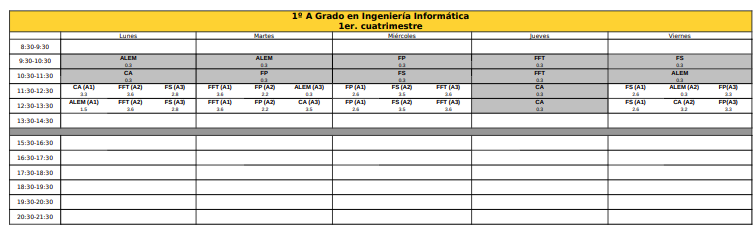
\includegraphics[width=0.8\textwidth]{figures/02_etsiit_horario.png}
                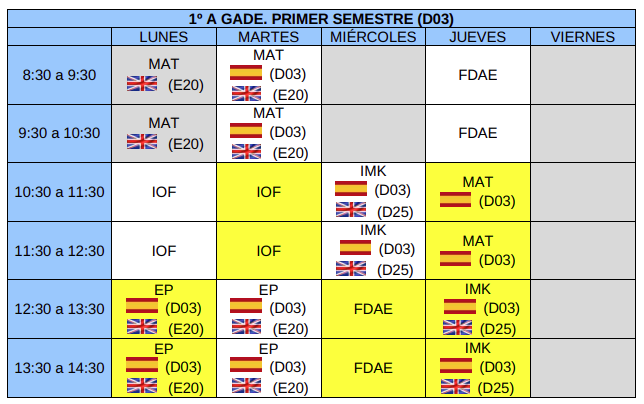
\includegraphics[width=0.8\textwidth]{figures/02_ade_horario.png}
                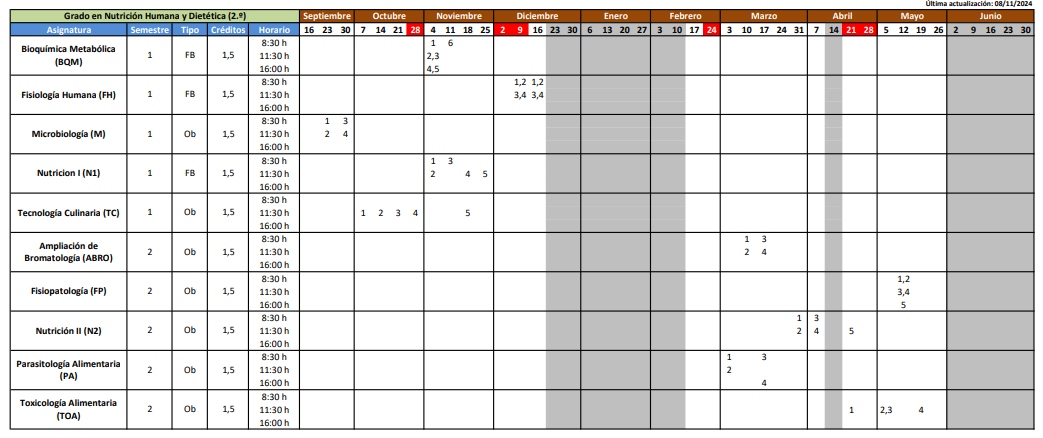
\includegraphics[width=0.8\textwidth]{figures/02_horario_doble_grado.png}
                \caption{Comparación de horarios de diferentes grados: ETSIIT (arriba), ADE (centro) y Doble Grado en Nutrición Humana y Dietética (abajo).}
                \label{fig:horarios_comparacion}
            \end{figure}
          

    \item A través de la web grados UGR \cite{webGrados} se puede buscar la información de los horarios de las asignaturas de los diferentes grados de la Universidad de Granada. Para ello debemos seleccionar rama de conocimiento, 
          grado, curso y asignatura. De esta manera obtenemos un horario semanal con las franjas horarias, aulas, profesores y fechas tanto de inicio como de fin. Este método nos proporcioan una interfaz estándar y más información, pero 
          también es más lento y tedioso para consultar por varias asignaturas o incluso grados.
    \item A través de las webs de cada departamento. Por ejemplo en la web del departamento de Ciencias de la Computación e Inteligencia Artificial \cite{webDecsai} se puede consultar la información de las asignaturas o profesores de este.
          Ofrece información adicional como asignaturas que imparte ``x'' profesor y su horario de tutorías y docencia.
\end{itemize}

Además para acceder a la información de periodos de actividad docente, exámenes finales, periodos de evaluación de convocatorias ... se ha de acceder a la web de la Secretaría General en la UGR \cite{webSecretaria} para consultar otro pdf.

En general la información de los horarios académicos de la Universidad de Granada es poco accesible, eficiente y consistente entre grados y facultades, lo que hace que el estudiante tenga que buscar la información de manera manual y tediosa.
Además no hay manera de consultar de manera sencilla un calendario personal que incluya tanto los horarios de las asignaturas como los exámenes y periodos de evaluación, entre otros.
\newline\newline
Pongamos el ejemplo de un estudiante matriculado en el primer curso del Grado de Biología en la Universidad de Granada con el estándar de cinco asignaturas en su primer cuatrimestre~\ref{fig:horario_biologia}. 
Este estudiante tiene que buscar la información de los horarios de las asignaturas en la web de su facultad, en la web de la Universidad de Granada o en la web del departamento al que pertenezca cada asignatura.
Suponemos que decide buscar su horario en la web de grados ugr, y una vez seleccionada la rama de conocimiento, grado, curso y asignatura, obtiene un horario semanal con las franjas horarias de todos los grupos de la asignatura, aulas, profesores y fechas tanto de inicio como de fin.
Está matriculado por ende en la asignatura ''Bases Químicas de la Biología'' en el grupo ``A'' de teoría y en el grupo ``2'' de prácticas, por lo que tiene que buscar los sectores que pertenecen a su grupos para poder obtener su horario personalizado para esa materia.
\newline\newline
La realidad con la que se encuentra el estudiante es con la siguiente:

\begin{figure}[H]
    \centering
    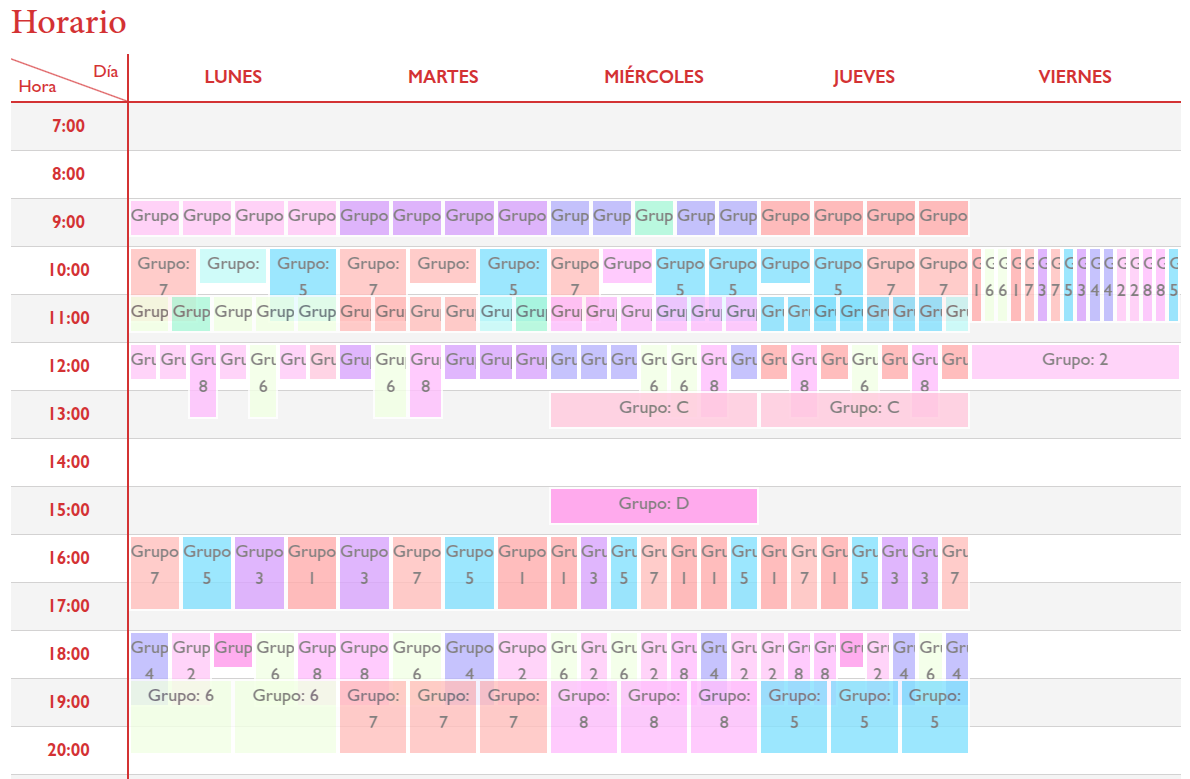
\includegraphics[width=0.8\textwidth]{figures/02_horario_biologia.png}
    \caption{Horario de la asignatura Bases Químicas de la Biología, impartida en el Grado en Biología.}
    \label{fig:horario_biologia}
\end{figure}

El estudiante tiene que dedicar un tiempo considerable en buscar las franjas pertenecientes a sus grupos, puesto que no hay una sencilla visualización de los mismos. Además se requiere una búsqueda activa con el cursor
para poder ver las franjas ocultas, y esta acción puede resultar tediosa cuando hay muchos sectores juntos, como en este caso.

Podemos concluir tras analizar la situación actual de aprovisionamiento de horarios académicos a los usuarios de la Universidad de Granada, que surge la necesidad de un sistema que permita la visualización de horarios académicos de manera sencilla, accesible y personalizada.

\section{Análisis comparativo de sistemas de planificación personalizada en educación superior}

Frente al modelo estático observado de manera generalizada en la Universidad de Granada, el panorama de la gestión de horarios en otras instituciones de educación superior y en el mercado de software educativo muestra una clara tendencia hacia sistemas más dinámicos, personalizados e integrados. 
\newline\newline
Existen diversas soluciones, desde módulos dentro de grandes sistemas ERP educativos hasta herramientas especializadas en la creación y gestión de horarios y planificadores académicos, pasando por aplicaciones de seguimiento del tiempo adaptadas al ámbito educativo.
El análisis de estas herramientas revela un conjunto de características comunes y avanzadas que definen el estado del arte en este dominio:

\begin{itemize}
      \item Por un lado ciertas universidades han desarrollado sistemas internos que permiten a los estudiantes acceder a sus horarios de manera personalizada, integrando información sobre asignaturas, grupos, aulas y profesores. Estos sistemas suelen ofrecer una interfaz gráfica intuitiva y accesible,
      permitiendo a los usuarios visualizar su horario de manera clara y sencilla. 

      %% 2 jpeg one next to the other

      \begin{figure}[H]
            \centering
            \makebox[\textwidth][c]{%
                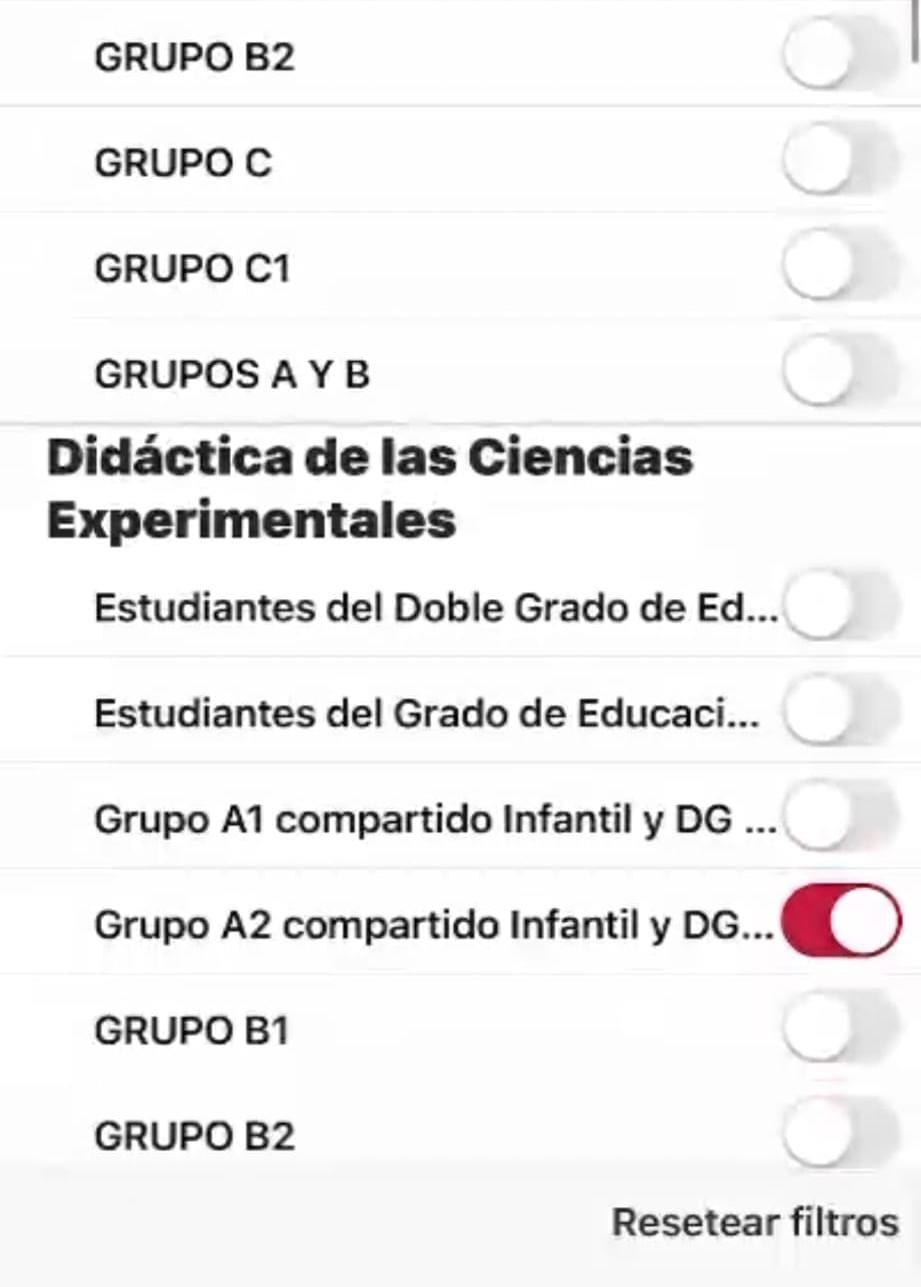
\includegraphics[height=8cm]{figures/03_ual_app_filtros.jpeg}
                \hspace{2cm}
                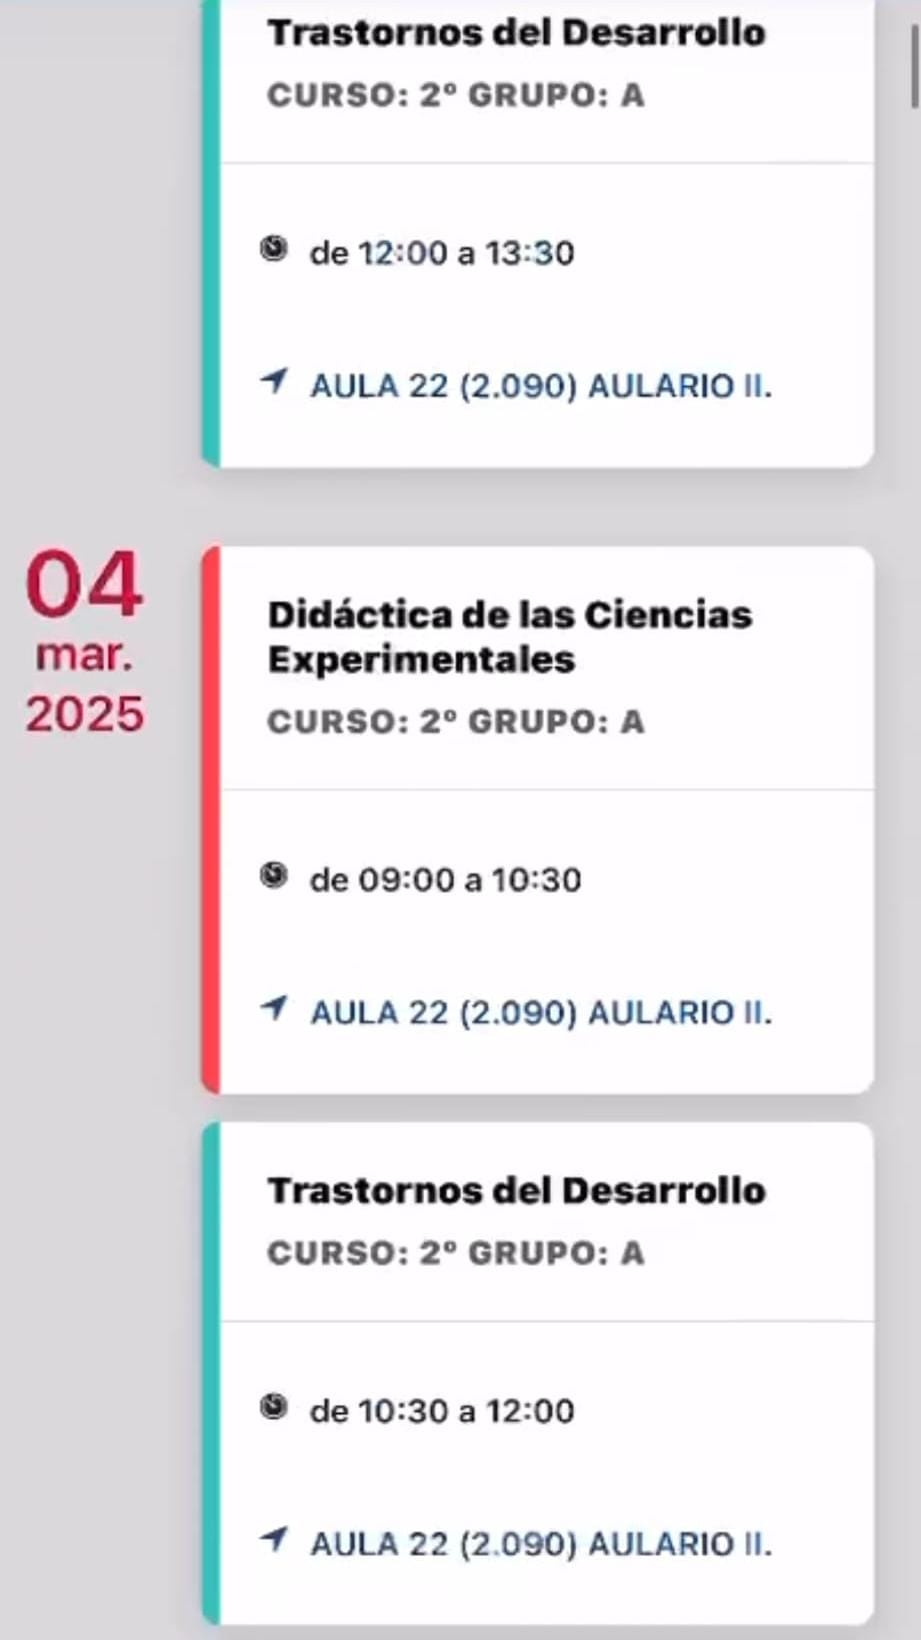
\includegraphics[height=8cm]{figures/03_ual_app_horarios.jpeg}
            }
            \caption{Aplicación móvil de la Universidad de Almería (UAL App).}
            \label{fig:ual_app}
        \end{figure}

      Exponiendo un ejemplo, la Universidad de Almeria (UAL) ha impementado en su aplicación móvil multiplataforma ``UAL App''~\ref{fig:ual_app}, la posibilidad de, seleccionando las asignaturas y grupos en los que se está matriculado, obtener
      una lista de las actividades ordenadas por hora según el día de la semana.
      \newline
      De esta manera en la misma aplicación que los estudiantes usan para consultar sus notas, expediente académico, días festivos, etc. pueden consultar su horario académico de manera rápida en el mismo ecosistema.

      \item Por otro lado, y de manera externa a las universidades, existen aplicaciones de gestión de horarios y planificación personal que permiten a los estudiantes integrar sus horarios académicos con otras actividades personales, como trabajos, eventos sociales o compromisos familiares. 
      \newline\newline
      Estas aplicaciones suelen ofrecer funciones avanzadas de recordatorios, notificaciones y sincronización con calendarios digitales, lo que facilita la organización del tiempo y la gestión de tareas.
      Un ejemplo representativo de este tipo de sistemas es 'My Study Life' \cite{webMyStudyLife}, una aplicación multiplataforma que permite a los estudiantes gestionar sus horarios académicos, tareas y exámenes de manera integrada~\ref{fig:mystudylife}. En este caso el sistema en sí no cuenta cona los datos internos de la universidad, sino que el estudiante tiene que introducir manualmente los datos de sus asignaturas y grupos, sin embargo, ofrece una interfaz intuitiva y fácil de usar, permitiendo a los estudiantes visualizar su horario de manera clara y sencilla.
      Además de la posibilidad de añadir tareas y exámenes, la aplicación permite establecer recordatorios y notificaciones para ayudar a los estudiantes a mantenerse organizados y cumplir con sus plazos, y es posee widgets personalizados para la pantalla de inicio de los dispositivos móviles e incluso aplicaciones para smartwatch, lo que consigue una integración total con el ecosistema del usuario.

      \begin{figure}[H]
            \centering
            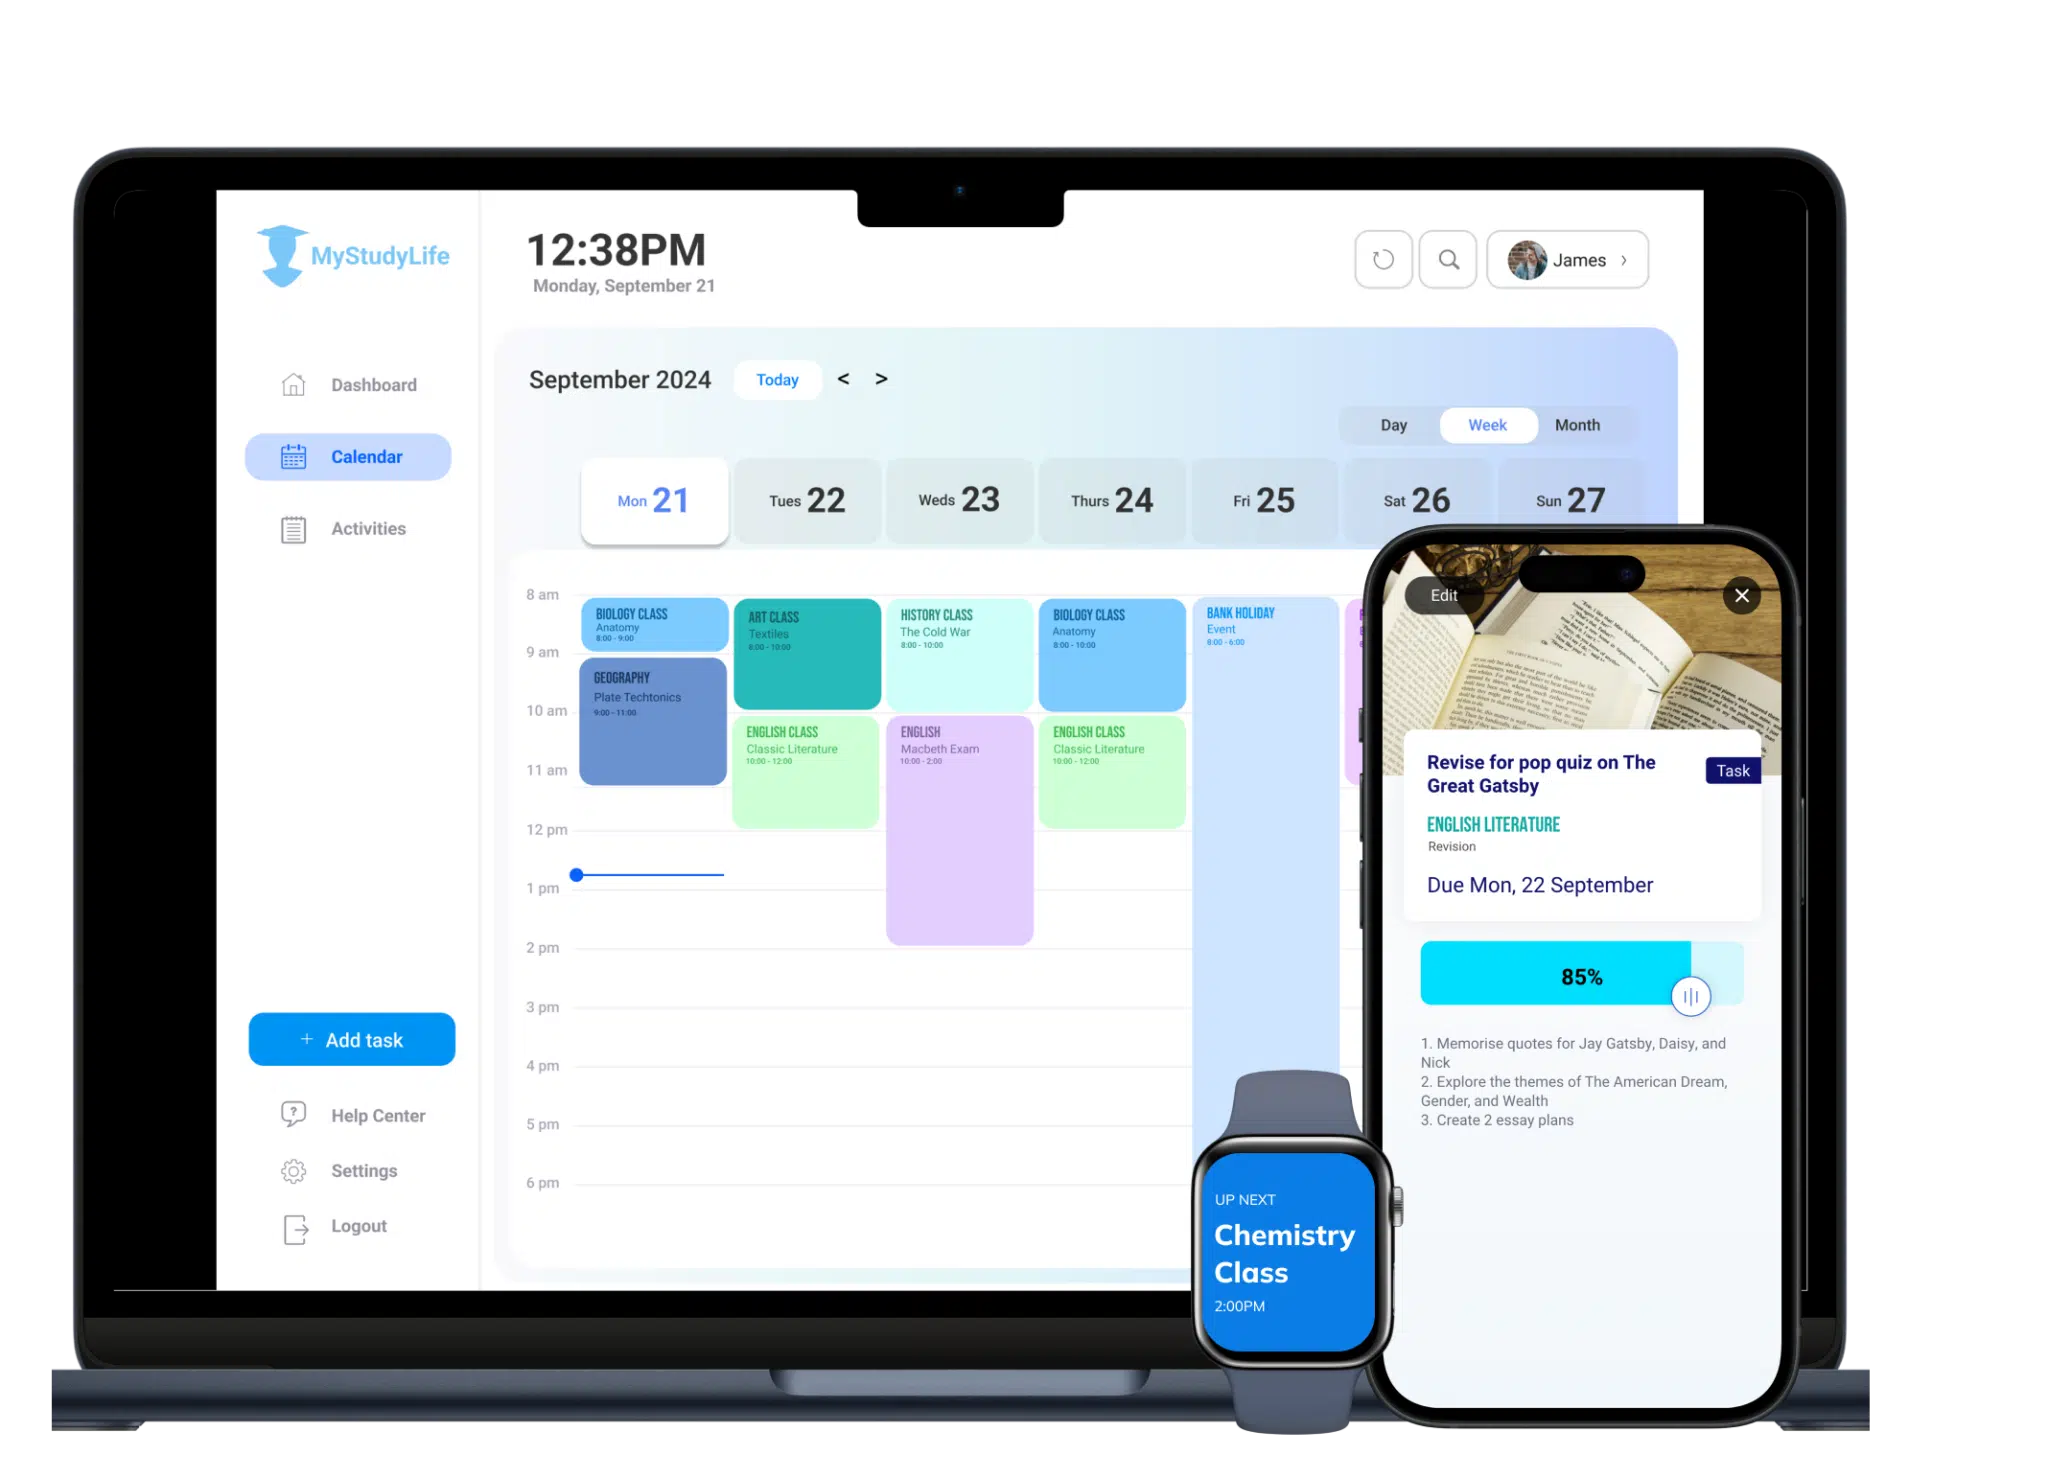
\includegraphics[width=0.8\textwidth]{figures/03_my_study_life.png}
            \caption{Aplicación My Study Life.}
            \label{fig:mystudylife}
      \end{figure}

      De manera general, y de uso más extendido, existen aplicaciones de gestión de tiempo y productividad que permiten a los usuarios organizar su tiempo de manera más eficiente como lo son Google Calendar \cite{webGoogleCalendar} o Microsoft Outlook \cite{webOutlook}.
      Estas aplicaciones permiten a los usuarios crear eventos, establecer recordatorios y sincronizar sus calendarios con otros dispositivos y aplicaciones. Sin embargo, no están específicamente diseñadas para la gestión de horarios académicos y pueden carecer de algunas funciones avanzadas que ofrecen otras aplicaciones más especializadas.
      Sin embargo también son usados para, sincronizando calendarios de sisemas externos, centralizar la información de los horarios académicos y otras actividades personales en un solo lugar, lo que facilita la gestión del tiempo y la planificación de tareas.

      \item Por último, existen sistemas de gestión de horarios y planificación académica que se integran con plataformas de aprendizaje en línea y sistemas de gestión del aprendizaje \hyperlink{lms}{LMS}, como Moodle \cite{webMoodle} o Blackboard.
      Estos sistemas permiten a los estudiantes acceder a su horario académico y a la información relacionada con sus cursos de manera centralizada, facilitando la gestión de tareas, exámenes y actividades académicas.
      Un ejemplo de este tipo de sistemas es el módulo de planificación académica de Moodle que permite a los estudiantes visualizar su horario académico y gestionar sus tareas y exámenes de manera integrada con la plataforma de aprendizaje.
      \newline\newline
      Este módulo ofrece una interfaz gráfica intuitiva y accesible, permitiendo a los estudiantes personalizar su horario académico y acceder a la información relacionada con sus cursos de manera centralizada. Además, el módulo de planificación académica de Moodle permite a los estudiantes establecer recordatorios y notificaciones para ayudarles a mantenerse organizados y cumplir con sus plazos.
      \newline\newline
      Sin embargo, este tipo de sistemas suelen estar limitados a las plataformas de aprendizaje en línea y no ofrecen la misma flexibilidad y personalización que otras aplicaciones de gestión de horarios y planificación personal.

\end{itemize}

\section{Desarrollo de servicios web}\label{sec:desarrollo_servicios_web}

El desarrollo de servicios web ha evolucionado significativamente en los últimos años, impulsado por la creciente demanda de aplicaciones distribuidas y la necesidad de integrar sistemas heterogéneos. En este contexto, se han desarrollado diferentes paradigmas arquitectónicos y tecnologías que permiten la creación de servicios web eficientes y escalables.

Esta evoluci\'{o}n ha llevado a una clara distinci\'{o}n de responsabilidades en el desarrollo de aplicaciones web, consolidando los conceptos de \hyperlink{frontend}{Frontend} y \hyperlink{backend}{Backend} como pilares fundamentales.

El \textbf{frontend}, tambi\'{e}n conocido como el "lado del cliente", es la parte de la aplicaci\'{o}n con la que el usuario interact\'{u}a directamente. Abarca la interfaz de usuario (\hyperlink{ui}{UI}), la experiencia de usuario (\hyperlink{ux}{UX}) y toda la l\'{o}gica que se ejecuta en el navegador web del cliente. Las tecnolog\'{i}as predominantes en el desarrollo frontend incluyen HTML para la estructura, CSS para la presentaci\'{o}n y JavaScript para la interactividad. 
\newline\newline
En los \'{u}ltimos a\~{n}os, frameworks y bibliotecas de JavaScript como React, Angular y Vue.js han ganado una enorme popularidad, permitiendo la creaci\'{o}n de interfaces de usuario din\'{a}micas, complejas y reutilizables. Estos frameworks facilitan la gesti\'{o}n del estado de la aplicaci\'{o}n en el cliente y la comunicaci\'{o}n as\'{i}ncrona con el servidor, mejorando la fluidez y la reactividad de las aplicaciones web modernas.

Por otro lado, el \textbf{backend}, o "lado del servidor", es el motor que impulsa la aplicaci\'{o}n. Se encarga de la l\'{o}gica de negocio, el procesamiento de datos, la autenticaci\'{o}n de usuarios, la gesti\'{o}n de bases de datos y la comunicaci\'{o}n con otros sistemas o servicios. Es invisible para el usuario final, pero crucial para el funcionamiento de la aplicaci\'{o}n. Existe una amplia variedad de lenguajes y frameworks para el desarrollo backend, como Node.js (con Express.js o NestJS), Python (con Django o Flask), Java (con Spring), Ruby (con Ruby on Rails), PHP (con Laravel o Symfony) y C\# (con .NET). La elecci\'{o}n de la tecnolog\'{i}a backend suele depender de factores como los requisitos de rendimiento, la escalabilidad, la experiencia del equipo de desarrollo y el ecosistema existente. El backend tambi\'{e}n es responsable de la seguridad de la aplicaci\'{o}n, implementando medidas para proteger los datos y prevenir accesos no autorizados.

La comunicaci\'{o}n entre el frontend y el backend se ha estandarizado en gran medida a trav\'{e}s de las \textbf{Interfaces de Programaci\'{o}n de Aplicaciones (\hyperlink{api}{API})}. 

Las Apis son vitales para la creación de experiencias digitales modernas, ya que simplifican como los sistemas se comunican, ofreciendo flexibilidad e independencia a una empresa. El mundo de las APIs está en constante evoluvión, y cada vez más empresas están adoptando este enfoque para integrar sus sistemas y servicios. Las APIs permiten a los desarrolladores acceder a funcionalidades específicas de una aplicación o servicio sin necesidad de conocer su implementación interna, lo que facilita la creación de aplicaciones complejas y la integración de diferentes sistemas.
\newline
Son cuatro tecnologías las que se han estandarizado como las más utilizadas para la creación de APIs: REST, SOAP, GraphQL y gRPC.

\begin{enumerate}
    \item \textbf{\hyperlink{rest}{REST} - El Estándar Atemporal}
    \begin{itemize}
        \item \textbf{Ventajas:} Maduro y ampliamente adoptado, simple y flexible, sin estado, múltiples tipos de medios.
        \item \textbf{Limitaciones:} Sobre-recuperación y sub-recuperación, complejidad de versionado, capacidades de tiempo real limitadas.
        \item \textbf{Mejores Casos de Uso:} APIs públicas, operaciones CRUD simples, requisitos de tiempo real limitados.
        \item \textbf{Consideraciones:} Versionado y escalabilidad para grandes bases de usuarios, impacto de la sobre/sub-recuperación.
    \end{itemize}

    \item \textbf{\hyperlink{soap}{SOAP} - El Clásico Empresarial}
    \begin{itemize}
        \item \textbf{Ventajas:} Protocolo estandarizado, seguridad robusta (WS-Security), transacciones y confiabilidad.
        \item \textbf{Limitaciones:} Verbosidad, complejidad, menor flexibilidad que REST.
        \item \textbf{Mejores Casos de Uso:} Sistemas empresariales, integraciones complejas, requisitos de seguridad estrictos.
        \item \textbf{Consideraciones:} Complejidad del protocolo y herramientas, justificación del uso frente a REST.
    \end{itemize}

    \item \textbf{\hyperlink{graphql}{GraphQL} - El Orquestador Dinámico}
    \begin{itemize}
        \item \textbf{Ventajas:} Obtención de datos impulsada por el cliente (reduce la sobre-recuperación), relaciones de datos complejas eficientes, actualizaciones en tiempo real (subscriptions), esquema flexible.
        \item \textbf{Limitaciones:} Mayor complejidad del servidor, curva de aprendizaje, ecosistema de herramientas en evolución.
        \item \textbf{Mejores Casos de Uso:} Aplicaciones de una sola página (SPAs), estructuras de datos complejas, actualizaciones y suscripciones en tiempo real.
        \item \textbf{Consideraciones:} Complejidad del servidor e impacto en el rendimiento, documentación y herramientas para desarrolladores.
    \end{itemize}

    \item \textbf{\hyperlink{grpc}{gRPC} - El Conducto de Alto Rendimiento}
    \begin{itemize}
        \item \textbf{Ventajas:} Alto rendimiento (HTTP/2, Protocol Buffers), soporte de streaming, fuertemente tipado, herramientas maduras.
        \item \textbf{Limitaciones:} Curva de aprendizaje más pronunciada, menos flexible, adopción menos extendida.
        \item \textbf{Mejores Casos de Uso:} Comunicación entre microservicios de alto rendimiento, escenarios de streaming, operaciones intensivas en datos.
        \item \textbf{Consideraciones:} Complejidad de adopción de gRPC y Protocol Buffers, justificación del esfuerzo de desarrollo por las ganancias de rendimiento.
    \end{itemize}
\end{enumerate}

Las \textbf{APIs REST (Representational State Transfer)}, estrategia a seguir para la creación del backend del proyecto, se han convertido en el paradigma dominante para dise\~{n}ar estas interfaces debido a su simplicidad, escalabilidad y flexibilidad. Una API REST define un conjunto de reglas y convenciones para que los sistemas puedan comunicarse a trav\'{e}s del protocolo HTTP.

La creaci\'{o}n de una API REST que sirva al frontend implica varios pasos clave:

\begin{itemize}
    \item \textbf{Definici\'{o}n de Recursos:} Se identifican los recursos que la API expondr\'{a} (por ejemplo, usuarios, productos, pedidos). Cada recurso tiene una URI (Uniform Resource Identifier) \'{u}nica.
    \item \textbf{Uso de M\'{e}todos HTTP \cite{MDNHTTPMethods2025}:} HTTP define un conjunto de métodos de petición para indicar la acción que se desea realizar para un recurso determinado. Aunque estos también pueden ser sustantivos, estos métodos de solicitud a veces son llamados HTTP verbs. Cada uno de ellos implementan una semántica diferente, pero algunas características similares son compartidas por un grupo de ellos: ej. un request method puede ser safe, idempotent, o cacheable.
    \newline\newline
    Los más usados son :
    \begin{itemize}
        \item \texttt{GET}: Solicita una representación de un recurso específico. Las peticiones que usan el método GET sólo deben recuperar datos.
        \item \texttt{HEAD}: Similar a GET, pero no devuelve el cuerpo de la respuesta, solo los encabezados. Se utiliza para obtener metadatos.
        \item \texttt{POST}: Se utiliza para enviar una entidad a un recurso en específico, causando a menudo un cambio en el estado o efectos secundarios en el servidor.
        \item \texttt{PUT}: Reemplaza todas las representaciones actuales del recurso de destino con la carga útil de la petición.
        \item \texttt{PATCH}: Aplica modificaciones parciales a un recurso.
        \item \texttt{OPTIONS}: Describe las opciones de comunicación para el recurso de destino. Permite al cliente conocer las capacidades del servidor.
        \item \texttt{DELETE}: Borra un recurso en específico.
    \end{itemize}
    \item \textbf{Representaci\'{o}n de Datos:} Los datos intercambiados entre el cliente y el servidor suelen estar en formato JSON (JavaScript Object Notation) debido a su ligereza y facilidad de parseo por parte de los navegadores y la mayor\'{i}a de los lenguajes de programaci\'{o}n. XML tambi\'{e}n puede ser utilizado, aunque es menos com\'{u}n en APIs modernas orientadas a frontend.
    \item \textbf{Statelessness (Ausencia de Estado):} Cada petici\'{o}n del cliente al servidor debe contener toda la informaci\'{o}n necesaria para que el servidor la entienda y procese. El servidor no almacena ning\'{u}n estado de la sesi\'{o}n del cliente entre peticiones. Esto simplifica el dise\~{n}o del servidor y mejora la escalabilidad.
    \item \textbf{Uso de C\'{o}digos de Estado HTTP:} Se utilizan c\'{o}digos de estado HTTP para indicar el resultado de una petici\'{o}n (por ejemplo, \texttt{200 OK}, \texttt{201 Created}, \texttt{400 Bad Request}, \texttt{401 Unauthorized}, \texttt{404 Not Found}, \texttt{500 Internal Server Error}).
\end{itemize}

El backend desarrolla estos endpoints de la API REST, implementando la l\'{o}gica necesaria para cada operaci\'{o}n. El frontend, a su vez, realiza peticiones HTTP (utilizando APIs del navegador como \texttt{Fetch} o bibliotecas como Axios) a estas URLs para enviar y recibir datos, actualizando din\'{a}micamente la interfaz de usuario sin necesidad de recargar la p\'{a}gina completa. Este desacoplamiento entre frontend y backend permite que ambos puedan desarrollarse, probarse, desplegarse y escalarse de forma independiente, facilitando la colaboraci\'{o}n entre equipos y la adopci\'{o}n de diferentes tecnolog\'{i}as para cada capa. Adem\'{a}s, una API REST bien dise\~{n}ada puede servir no solo a una aplicaci\'{o}n web, sino tambi\'{e}n a aplicaciones m\'{o}viles u otros servicios, promoviendo la reutilizaci\'{o}n y la interoperabilidad entre sistemas heterog\'{e}neos, tal como se mencionaba al inicio.

La tendencia hacia arquitecturas de microservicios en el backend ha reforzado a\'{u}n m\'{a}s la importancia de las APIs REST bien definidas, ya que cada microservicio suele exponer su funcionalidad a trav\'{e}s de una API. En este contexto, herramientas como OpenAPI (anteriormente Swagger) para la definici\'{o}n y documentaci\'{o}n de APIs, y soluciones de API Gateway para la gesti\'{o}n, seguridad y monitorizaci\'{o}n del tr\'{a}fico de las APIs, se han vuelto indispensables en el desarrollo de servicios web modernos y robustos.

\subsection{Arquitecturas de software}

La elección de la arquitectura backend es una decisión fundamental en el desarrollo de cualquier aplicación web, impactando directamente en su escalabilidad, mantenibilidad, flexibilidad y velocidad de desarrollo. Para un sistema de gestión de horarios académicos como el propuesto, que potencialmente puede crecer en complejidad y número de usuarios, la comparación entre los enfoques monolítico y de microservicios es particularmente relevante.

Si bien la arquitectura monolítica ha sido tradicionalmente un punto de partida, la creciente complejidad de los sistemas y la necesidad de agilidad han impulsado la adopción y evolución de diversos paradigmas arquitectónicos. A continuación, se presenta una exposición de diferentes arquitecturas de software \cite{bookORellySoftwareArchitecture} implementadas en sistemas backend, analizando sus características y su posición en el espectro que va desde el monolito hasta los microservicios.

\subsubsection*{Arquitectura en Capas (Layered Architecture / N-Tier Architecture) \cite{clean_architecture}}

\begin{description}
    \item[\textbf{Descripción:}] Este es uno de los patrones arquitectónicos más establecidos y fundamentales. Consiste en la organización del código en capas horizontales, donde cada capa posee una responsabilidad específica y se comunica, por lo general, únicamente con las capas adyacentes (superior e inferior). Las capas típicas suelen ser:
    \begin{itemize}
        \item \textit{Capa de Presentación (o Interfaz de Usuario):} Gestiona la interacción con el usuario o sistemas cliente. En el contexto de un backend, esta capa a menudo se materializa como la API que gestiona las solicitudes HTTP.
        \item \textit{Capa de Aplicación (o Lógica de Negocio):} Contiene la lógica de negocio central y orquesta las tareas y flujos de trabajo.
        \item \textit{Capa de Dominio (o Modelo de Negocio):} Representa las entidades, los objetos de valor y las reglas inherentes al dominio del negocio.
        \item \textit{Capa de Acceso a Datos (o Persistencia):} Encargada de la comunicación con los sistemas de almacenamiento de datos, como bases de datos.
        \item \textit{Capa de Infraestructura:} Provee servicios técnicos transversales, tales como logging, monitorización, y comunicación de red.
    \end{itemize}
    \item[\textbf{Posicionamiento y Evolución:}] Una aplicación monolítica frecuentemente se estructura internamente siguiendo una arquitectura en capas. Aunque este patrón no descompone el sistema en servicios desplegables de forma independiente, sí promueve una modularización interna y una clara separación de responsabilidades (Separation of Concerns), lo cual es un primer paso crucial para gestionar la complejidad y facilitar la mantenibilidad de un sistema antes de considerar arquitecturas más distribuidas.
\end{description}

\subsubsection*{Arquitectura Orientada a Servicios (SOA - Service-Oriented Architecture) \cite{soa_ibm}}

\begin{description}
    \item[\textbf{Descripción:}] SOA es un paradigma de diseño que estructura una aplicación como una colección de servicios que se comunican entre sí. Estos servicios encapsulan funcionalidades de negocio discretas y pueden ser accedidos a través de la red. A menudo, los servicios en SOA son de grano más grueso en comparación con los microservicios. La comunicación se estandarizó frecuentemente mediante protocolos como SOAP (Simple Object Access Protocol) sobre HTTP, y es común el uso de un Enterprise Service Bus (ESB) para la mediación, el enrutamiento y la transformación de mensajes entre servicios.
    \item[\textbf{Características Clave:}] Fomenta la reutilización de servicios a nivel empresarial, la interoperabilidad entre sistemas heterogéneos y el descubrimiento dinámico de servicios.
    \item[\textbf{Posicionamiento y Evolución:}] SOA representó un avance significativo respecto a los monolitos, permitiendo una descomposición más formal y orientada a negocio. Puede considerarse un precursor importante de la arquitectura de microservicios. Sin embargo, SOA a menudo implicaba una mayor sobrecarga en términos de estándares, una gobernanza más centralizada y, en ocasiones, cuellos de botella debidos al ESB, aspectos que la arquitectura de microservicios busca simplificar o descentralizar.
\end{description}

\subsubsection*{Arquitectura Dirigida por Eventos (EDA - Event-Driven Architecture) \cite{aws_eda}}

\begin{description}
    \item[\textbf{Descripción:}] En una EDA, el flujo de la aplicación es determinado por la ocurrencia de eventos. Los eventos son notificaciones que representan un cambio de estado significativo o un suceso relevante dentro del sistema (por ejemplo, ``PedidoRealizado'', ``InventarioBajo''). Los componentes del sistema, denominados productores de eventos, publican estos eventos en un canal o bus de eventos (gestionado por un bróker de mensajes como Apache Kafka, RabbitMQ o Google Cloud Pub/Sub). Otros componentes, los consumidores de eventos, se suscriben a los eventos que les conciernen y reaccionan a ellos de forma asíncrona.
    \item[\textbf{Estilos Principales:}] Se distinguen dos topologías principales: el \textit{mediador de eventos}, donde un componente central orquesta el flujo de eventos, y el \textit{bróker de eventos}, que facilita una mayor desacoplamiento entre publicadores y suscriptores.
    \item[\textbf{Posicionamiento y Evolución:}] EDA es altamente compatible y a menudo se utiliza en conjunción con la arquitectura de microservicios para lograr una comunicación asíncrona, resiliente y escalable. Permite un desacoplamiento profundo entre servicios, mejorando la tolerancia a fallos y la capacidad de respuesta del sistema. También se emplea para modernizar sistemas monolíticos, permitiendo integrar nuevas funcionalidades de forma reactiva o desacoplar módulos existentes.
\end{description}

\subsubsection*{Arquitectura ``Serverless'' y Nativa de la Nube \cite{aws_serverless}}
\begin{description}
    \item[\textbf{Descripción:}] Este enfoque se centra en la ejecución de código sin necesidad de gestionar servidores o infraestructura subyacente. Los desarrolladores escriben funciones que se ejecutan en respuesta a eventos, y el proveedor de la nube (como AWS Lambda, Azure Functions o Google Cloud Functions) se encarga de la infraestructura, escalabilidad y disponibilidad. Las aplicaciones nativas de la nube están diseñadas para aprovechar al máximo las capacidades de la nube, como el escalado automático, la alta disponibilidad y los servicios gestionados.
    \item[\textbf{Características Clave:}] Despliegue basado en funciones, escalabilidad automática, pago por uso (se paga solo por el tiempo de ejecución), y enfoque en eventos y microservicios.
    \item[\textbf{Posicionamiento y Evolución:}] La arquitectura serverless es una evolución natural hacia una mayor abstracción y simplificación del desarrollo backend. Permite a los equipos centrarse en la lógica de negocio sin preocuparse por la infraestructura subyacente. Sin embargo, puede introducir desafíos relacionados con el estado, la latencia y el control sobre el entorno de ejecución.
    Este enfoque es especialmente adecuado para aplicaciones que requieren escalabilidad extrema y una alta disponibilidad, como sistemas de gestión de horarios académicos que pueden experimentar picos de carga durante períodos específicos (por ejemplo, al inicio del semestre).
\end{description}

\subsubsection*{Arquitectura de Microservicios \cite{ms_microservices}}

\begin{description}
    \item[\textbf{Descripción:}] Esta arquitectura estructura una aplicación como una suite de pequeños servicios independientes, cada uno enfocado en una capacidad de negocio específica y bien delimitada (Bounded Context). Cada microservicio es autónomo, lo que implica que puede ser desarrollado, desplegado, escalado y gestionado de forma independiente. Típicamente, cada servicio posee su propia base de datos para asegurar un bajo acoplamiento y se comunica con otros servicios a través de APIs ligeras y bien definidas, comúnmente utilizando HTTP/REST, gRPC, o a través de mensajería asíncrona.
    \item[\textbf{Características Clave:}] Despliegue independiente y continuo, escalabilidad granular (se escalan solo los servicios que lo necesitan), flexibilidad tecnológica (posibilidad de usar diferentes stacks tecnológicos por servicio), aislamiento de fallos (un fallo en un servicio no debería derribar todo el sistema), y alineación con equipos de desarrollo pequeños y autónomos (Conway's Law).
    \item[\textbf{Posicionamiento y Evolución:}] La arquitectura de microservicios se considera una evolución directa y una alternativa robusta para superar las limitaciones intrínsecas de los sistemas monolíticos, especialmente en contextos de alta complejidad, crecimiento rápido y necesidad de agilidad. Aborda desafíos como la dificultad para escalar, la complejidad en el mantenimiento, la lentitud en la adopción de nuevas tecnologías, los ciclos de despliegue prolongados y el alto acoplamiento que caracterizan a las grandes aplicaciones monolíticas.
\end{description}

\subsubsection*{Conclusión: Progresión y Criterios de Selección}

El panorama de arquitecturas backend ha evolucionado desde la simplicidad inicial de los sistemas \textbf{monolíticos}, pasando por la modularización interna de la \textbf{arquitectura en capas}, hacia la descomposición en servicios con \textbf{SOA}. Posteriormente, paradigmas como la \textbf{arquitectura dirigida por eventos} han ganado tracción para mejorar el desacoplamiento y la resiliencia, mientras que enfoques como la \textbf{arquitectura basada en el espacio} y los \textbf{principios nativos de la nube} abordan la escalabilidad extrema y la eficiencia en entornos cloud.

Finalmente, la \textbf{arquitectura de microservicios}, arquitectura a adoptar en el backend del sistema, emerge como un enfoque predominante para construir sistemas complejos, distribuidos y altamente escalables, ofreciendo un alto grado de agilidad y autonomía. No obstante, es crucial destacar que no existe una arquitectura universalmente superior. La selección de la arquitectura más adecuada debe ser el resultado de un análisis cuidadoso de los requisitos específicos del proyecto, el contexto del negocio, las capacidades del equipo de desarrollo, las proyecciones de escalabilidad y los compromisos (trade-offs) inherentes a cada patrón. En muchos sistemas del mundo real, es común encontrar combinaciones pragmáticas de estos patrones arquitectónicos.

\subsection{Tecnologías de desarrollo}

En el ámbito del desarrollo de software, la elección de las tecnologías adecuadas es crucial para el éxito de un proyecto. En este apartado, se presentan las principales tecnologías que se han considerado para el desarrollo del sistema de gestión de horarios académicos.

\subsubsection{Tecnologías y lenguajes backend}

\begin{enumerate}
    \item \textbf{Java con Spring Framework (Spring Boot y Spring Cloud)\cite{springcloud}:}
    Java es un lenguaje de programación robusto, maduro y ampliamente adoptado en el desarrollo de aplicaciones empresariales a gran escala. Su ecosistema es vasto, con una gran comunidad y un fuerte enfoque en el rendimiento y la seguridad. Spring Boot simplifica drásticamente la creación de aplicaciones basadas en Spring, ofreciendo auto-configuración, servidores web embebidos (como Tomcat o Jetty) y una gestión de dependencias simplificada, lo que lo convierte en una opción popular para el desarrollo rápido de microservicios listos para producción. De hecho, se considera el estándar de facto para microservicios en Java.

    Para arquitecturas de microservicios, Spring Cloud complementa a Spring Boot proporcionando un conjunto de herramientas y patrones para construir sistemas distribuidos resilientes y escalables. Esto incluye soluciones para el descubrimiento de servicios (permitiendo que los servicios se encuentren dinámicamente en la red), balanceo de carga (distribuyendo las solicitudes entre múltiples instancias de un servicio), pasarelas API (un punto de entrada único para todas las solicitudes de los clientes), interruptores de circuito (para prevenir fallos en cascada) y gestión de configuración distribuida. Dada la potencial complejidad de un sistema de gestión de horarios universitarios, especialmente si se opta por microservicios, la madurez y el soporte integral de Spring Cloud para estos patrones son altamente relevantes.

    \item \textbf{.NET Core\cite{dotnetcore}:}
    .NET Core (ahora parte de .NET 5 y versiones posteriores) es un framework de desarrollo de aplicaciones multiplataforma, de código abierto y de alto rendimiento mantenido por Microsoft. Es una opción sólida para construir microservicios, con excelente soporte para la creación de APIs RESTful, contenedores Docker y despliegue en plataformas de orquestación como Kubernetes. Ofrece características como escalabilidad, un modelo de entrega continua, herramientas para operaciones CRUD, soporte para comunicación síncrona y asíncrona entre servicios, y la implementación de patrones de diseño avanzados como CQRS (Command and Query Responsibility Segregation) y Event Sourcing. También se integra bien con tecnologías de caché como Redis y proporciona mecanismos de seguridad robustos mediante OAuth2 y OpenID Connect. Para equipos con experiencia en el ecosistema Microsoft o que buscan una alternativa de alto rendimiento a Java, .NET Core es una opción muy competente.

    \item \textbf{Node.js con Express.js\cite{expressjs}:}
    Node.js es un entorno de ejecución para JavaScript del lado del servidor, construido sobre el motor V8 de Chrome. Su principal característica distintiva es su modelo de E/S (Entrada/Salida) asíncrono y sin bloqueo, orientado a eventos. Esto lo hace particularmente eficiente para aplicaciones que manejan un gran número de conexiones concurrentes y operaciones de E/S intensivas, como aplicaciones en tiempo real o APIs que actúan como fachadas para otros servicios. Express.js es un framework web minimalista y flexible para Node.js, ampliamente utilizado para construir APIs RESTful y microservicios ligeros. Su simplicidad y el vasto ecosistema de paquetes disponibles a través de npm (Node Package Manager) permiten un desarrollo rápido. En el contexto de un sistema de gestión de horarios, Node.js con Express podría ser adecuado para microservicios específicos que se beneficien de su naturaleza asíncrona, como un servicio de notificaciones en tiempo real o una pasarela API ligera.

    \item \textbf{Python con Django/Flask\cite{djangobook}\cite{flask}:}
    Python es un lenguaje de programación conocido por su sintaxis clara, legibilidad y alta productividad del desarrollador.Para el desarrollo web, existen dos frameworks principales: Django y Flask. Django es un framework de ``baterías incluidas'' que proporciona muchas funcionalidades listas para usar, como un ORM (Object-Relational Mapper), un panel de administración y un sistema de autenticación. Esto puede acelerar el desarrollo de aplicaciones web completas. Flask, por otro lado, es un micro-framework que proporciona las herramientas esenciales para construir aplicaciones web, ofreciendo mayor flexibilidad y dejando más decisiones de diseño al desarrollador.

    Para microservicios, Flask es a menudo la opción preferida debido a su ligereza y minimalismo, permitiendo construir servicios pequeños y enfocados sin el overhead de Django. Sin embargo, Django podría considerarse si un microservicio específico se beneficia significativamente de sus características integradas. Ambos frameworks cuentan con comunidades maduras y un amplio soporte.

    \item \textbf{Consideraciones para la Elección del Stack Backend:}
    La elección del stack tecnológico para el backend está intrínsecamente ligada a la arquitectura general seleccionada (monolito o microservicios) y, de manera crucial, a la experiencia y familiaridad del equipo de desarrollo. Si se adopta una arquitectura de microservicios, frameworks con un robusto soporte para patrones de sistemas distribuidos, como Spring Cloud para el ecosistema Java, ofrecen ventajas considerables en términos de gestión y resiliencia. Por otro lado, si la velocidad de desarrollo inicial para un monolito o para microservicios más simples es prioritaria, alternativas como Python con Flask o Node.js con Express pueden permitir un arranque más rápido. La disponibilidad de desarrolladores con experiencia en un stack tecnológico particular, por ejemplo, Java en entornos corporativos o universitarios, puede ser un factor determinante, incluso si otro stack pudiera parecer marginalmente superior desde una perspectiva puramente técnica.

    Además, la ``madurez'' de un lenguaje y framework, como es el caso de Java y Spring, no solo implica estabilidad del código base, sino también la existencia de un vasto ecosistema de herramientas, bibliotecas probadas y soluciones documentadas para problemas comunes. Este ecosistema reduce el riesgo inherente al desarrollo y puede acortar los tiempos de desarrollo a largo plazo al evitar la necesidad de ``reinventar la rueda''. Para un sistema potencialmente complejo como la gestión de horarios académicos, que podría requerir integraciones con sistemas universitarios preexistentes, autenticación robusta y una gestión de datos sofisticada, la amplitud y profundidad de un ecosistema maduro pueden ser más beneficiosas que un framework más nuevo o ligero que exija más integraciones manuales o el desarrollo de componentes básicos desde cero.
\end{enumerate}

\subsubsection{Tecnologías y lenguajes frontend}

En el contexto de desarrollo web orientado al cliente, la elección de tecnologías y lenguajes es fundamental para garantizar una experiencia de usuario fluida y eficiente. A continuación, se presentan las principales tecnologías y lenguajes considerados para el desarrollo del frontend del sistema de gestión de horarios académicos.

En cuanto a lenguajes de programación, \textbf{JavaScript}\cite{javascript} es el lenguaje de programación más utilizado en el desarrollo frontend. Es un lenguaje interpretado y orientado a objetos que permite la creación de aplicaciones web interactivas y dinámicas. JavaScript se ejecuta en el navegador del cliente, lo que permite la manipulación del DOM (Document Object Model) y la interacción con el usuario sin necesidad de recargar la página.
\newline\newline
El \textbf{HTML (HyperText Markup Language)}\cite{html} es el lenguaje de marcado utilizado para estructurar el contenido de las páginas web. HTML define la estructura y el contenido de una página, incluyendo texto, imágenes, enlaces y otros elementos multimedia. Junto con CSS (Cascading Style Sheets), que se utiliza para definir la presentación y el diseño visual de las páginas web, HTML forma la base del desarrollo frontend.
\newline\newline
El \textbf{CSS}\cite{css} es un lenguaje de estilo utilizado para describir la presentación de un documento HTML. CSS permite definir el diseño, los colores, las fuentes y otros aspectos visuales de una página web. Junto con HTML y JavaScript, CSS forma el trinomio fundamental del desarrollo frontend.
\newline\newline
Respecto a frameworks y bibliotecas, existen varias opciones populares que facilitan el desarrollo frontend:   

\begin{enumerate}
    \item \textbf{React\cite{react}:} Es una biblioteca de JavaScript desarrollada por Facebook para construir interfaces de usuario. React se basa en componentes reutilizables y permite la creación de aplicaciones web dinámicas y escalables. Su enfoque basado en el estado y el ciclo de vida de los componentes facilita la gestión de la interactividad y la actualización eficiente del DOM.
    \item \textbf{Angular\cite{angular}:} Es un framework de desarrollo web desarrollado por Google que permite la creación de aplicaciones web de una sola página (SPA). Angular utiliza TypeScript, un superconjunto de JavaScript, y ofrece una arquitectura basada en componentes, inyección de dependencias y un sistema de enrutamiento robusto.
    \item \textbf{Vue.js\cite{vuejs}:} Es un framework progresivo para construir interfaces de usuario. Vue.js es fácil de integrar con otras bibliotecas o proyectos existentes y se centra en la capa de vista. Su enfoque reactivo y su sistema de componentes lo hacen adecuado para aplicaciones pequeñas y grandes.
\end{enumerate}

\subsection{Sistemas de almacenamiento de datos}

Los sistemas de almacenamiento de datos son fundamentales en el desarrollo de aplicaciones web, ya que permiten la persistencia y gestión eficiente de la información. En el contexto del sistema de gestión de horarios académicos, se han considerado varias opciones para el almacenamiento de datos.
\begin{enumerate}
    \item \textbf{Bases de Datos Relacionales (RDBMS):} Estas bases de datos utilizan un modelo tabular para almacenar datos y son ideales para aplicaciones que requieren transacciones complejas y relaciones entre datos. Ejemplos populares incluyen MySQL\cite{mysql}, PostgreSQL\cite{postgresql} y Microsoft SQL Server\cite{sqlserver}. Estas bases de datos son adecuadas para el sistema de gestión de horarios, ya que permiten la creación de relaciones entre entidades como grados, asignaturas, grupos y clases.\newline
        La ventaja de utilizar una base de datos relacional es la capacidad de realizar consultas complejas y garantizar la integridad referencial de los datos. Sin embargo, pueden presentar limitaciones en términos de escalabilidad horizontal ( agregar más servidores para manejar cargas de trabajo ) y flexibilidad en la estructura de datos.
    
    \item \textbf{Bases de Datos NoSQL:} Estas bases de datos son ideales para aplicaciones que requieren alta escalabilidad y flexibilidad en la estructura de datos. Existen varios tipos de bases de datos NoSQL, como bases de datos orientadas a documentos (MongoDB)\cite{mongodb}, bases de datos clave-valor (Redis)\cite{redis}, bases de datos en columna (Cassandra)\cite{cassandra} y bases de datos orientadas a grafos (Neo4j)\cite{neo4j}. Las bases de datos NoSQL son adecuadas para aplicaciones que manejan grandes volúmenes de datos no estructurados o semi-estructurados.\newline
        La ventaja de utilizar una base de datos NoSQL es la capacidad de escalar horizontalmente y manejar grandes volúmenes de datos. Sin embargo, pueden presentar limitaciones en términos de transacciones complejas y consistencia de datos.

    \item \textbf{Bases de Datos en Memoria:} Estas bases de datos almacenan datos en la memoria RAM, lo que permite un acceso extremadamente rápido. Son ideales para aplicaciones que requieren baja latencia y alto rendimiento, como sistemas de caché o análisis en tiempo real. Ejemplos populares incluyen Redis y Memcached\cite{memcached}.\newline
        La ventaja de utilizar una base de datos en memoria es la velocidad de acceso a los datos. Sin embargo, pueden presentar limitaciones en términos de persistencia de datos y capacidad de almacenamiento.

    \item \textbf{Bases de Datos en la Nube:} Estas bases de datos son ofrecidas como servicios en la nube y permiten a las empresas escalar y gestionar sus datos sin preocuparse por la infraestructura subyacente. Ejemplos populares incluyen Amazon RDS\cite{amazonrds}, Google Cloud SQL\cite{googlecloudsql} y Azure Cosmos DB\cite{azurecosmosdb}.\newline
        La ventaja de utilizar una base de datos en la nube es la escalabilidad y la facilidad de gestión. Sin embargo, pueden presentar limitaciones en términos de control sobre la infraestructura y costos a largo plazo.

    \item \textbf{Bases de Datos Híbridas:} Estas bases de datos combinan características de bases de datos relacionales y NoSQL, permitiendo a las aplicaciones aprovechar lo mejor de ambos mundos. Ejemplos populares incluyen Amazon Aurora\cite{amazonaurora} y Google Cloud Spanner\cite{cloudspanner}.\newline
        La ventaja de utilizar una base de datos híbrida es la flexibilidad y la capacidad de manejar diferentes tipos de datos. Sin embargo, pueden presentar limitaciones en términos de complejidad y costos.
\end{enumerate}

\subsection{Autenticación y autorización}

La autenticación y autorización son componentes críticos en el desarrollo de aplicaciones web, especialmente en sistemas que manejan datos sensibles o requieren control de acceso granular. En el contexto del sistema de gestión de horarios académicos, se han considerado varias opciones para implementar la autenticación y autorización.
\begin{enumerate}
    \item \textbf{Autenticación basada en formularios\cite{auth_form}:} Este es el método más común de autenticación en aplicaciones web. Los usuarios ingresan sus credenciales (nombre de usuario y contraseña) en un formulario, que se envía al servidor para su validación. Si las credenciales son correctas, el servidor crea una sesión y devuelve un token de sesión al cliente. Este token se utiliza para autenticar las solicitudes posteriores.\newline
        La ventaja de este método es su simplicidad y facilidad de implementación. Sin embargo, puede presentar limitaciones en términos de seguridad (por ejemplo, ataques de fuerza bruta) y experiencia del usuario (por ejemplo, necesidad de recordar contraseñas).
    \item \textbf{Autenticación basada en tokens\cite{auth_jwt}:} Este método utiliza tokens (como \hyperlink{jwt}{JWT} - JSON Web Tokens) para autenticar a los usuarios. Después de que el usuario ingresa sus credenciales, el servidor genera un token firmado y lo envía al cliente. Este token se incluye en las solicitudes posteriores para autenticar al usuario. La ventaja de este método es que no requiere mantener sesiones en el servidor, lo que facilita la escalabilidad y la interoperabilidad entre diferentes servicios, lo que casa a la perfección con el concepto de API REST anteriormente mencionado.\newline
        Sin embargo, puede presentar limitaciones en términos de seguridad (por ejemplo, tokens robados) y complejidad de implementación (por ejemplo, gestión de la expiración de tokens).
    \item \textbf{Autenticación basada en OAuth2\cite{auth_mfa}:} OAuth2 es un protocolo de autorización que permite a los usuarios otorgar acceso limitado a sus recursos a aplicaciones de terceros sin compartir sus credenciales. Este método es ampliamente utilizado por plataformas como Google, Facebook y Twitter para permitir el inicio de sesión único (\hyperlink{sso}{SSO}) en aplicaciones de terceros.\newline
        La ventaja de este método es su flexibilidad y capacidad para integrar múltiples proveedores de identidad. Sin embargo, puede presentar limitaciones en términos de complejidad de implementación y dependencia de terceros.
    \item \textbf{Autenticación multifactor (MFA)\cite{auth_oauth2}:} Este método combina múltiples factores de autenticación (ejemplo, contraseña y código enviado por SMS) para aumentar la seguridad. La ventaja de este método es su capacidad para prevenir accesos no autorizados incluso si las credenciales son comprometidas. Sin embargo, puede presentar limitaciones en términos de experiencia del usuario (por ejemplo, necesidad de ingresar múltiples factores) y complejidad de implementación.
    \item \textbf{Autenticación basada en LDAP\cite{auth_ldap}:} LDAP (Lightweight Directory Access Protocol) es un protocolo utilizado para acceder y gestionar servicios de directorio. Este método permite autenticar a los usuarios utilizando un servidor LDAP, que almacena información sobre usuarios y grupos. La ventaja de este método es su capacidad para integrar múltiples sistemas y aplicaciones. Sin embargo, puede presentar limitaciones en términos de complejidad de implementación y dependencia de terceros.    
\end{enumerate}

\subsection{Comunicación entre servicios}

La comunicación entre servicios es un aspecto fundamental en el desarrollo de aplicaciones distribuidas, especialmente en arquitecturas de microservicios. Existen varias opciones para implementar la comunicación entre servicios, cada una con sus ventajas y desventajas.\newline

EL paso de información entre servicios puede realizarse de diferentes maneras, dependiendo de la arquitectura y los requisitos del sistema. A continuación, se presentan las principales opciones para la comunicación entre servicios:

\begin{itemize}
    \item \textbf{Comunicación síncrona:} Este enfoque implica que un servicio realiza una solicitud a otro servicio y espera una respuesta antes de continuar. Los protocolos más comunes para la comunicación síncrona son HTTP/REST y gRPC. La ventaja de este enfoque es su simplicidad y facilidad de implementación. Sin embargo, puede presentar limitaciones en términos de latencia y disponibilidad, ya que un fallo en un servicio puede afectar a otros servicios que dependen de él.
    Tecnologías comunes (descritas en la sección \ref{sec:desarrollo_servicios_web}):  
    \begin{itemize}
        \item \textbf{HTTP/REST}\cite{http_rest}
        \item \textbf{SOAP}\cite{soap}
        \item \textbf{gRPC}\cite{grpc}
        \item \textbf{GraphQL}\cite{graphql}
    \end{itemize}
    \item \textbf{Comunicación asíncrona:} Este enfoque permite que un servicio envíe un mensaje a otro servicio sin esperar una respuesta inmediata. Los mensajes se envían a través de un sistema de mensajería (como RabbitMQ, Apache Kafka o Amazon SQS) y pueden ser procesados en paralelo por los servicios receptores. La ventaja de este enfoque es su capacidad para manejar cargas de trabajo variables y mejorar la resiliencia del sistema. Sin embargo, puede presentar limitaciones en términos de complejidad de implementación y gestión de errores.
    Tecnologías comunes:
    \begin{itemize}
        \item \textbf{RabbitMQ\cite{rabbitmq}:} RabbitMQ es un sistema de mensajería de código abierto que implementa el protocolo AMQP (Advanced Message Queuing Protocol). Permite la comunicación asíncrona entre servicios mediante el uso de colas de mensajes, lo que facilita la desacoplación y la escalabilidad.
        Tiene la capacidad de manejar grandes volúmenes de mensajes y ofrece características como confirmaciones de entrega, enrutamiento avanzado y soporte para múltiples protocolos de mensajería, como MQTT y STOMP.
        \item \textbf{Apache Kafka\cite{kafka}:} Kafka es una plataforma de mensajería distribuida diseñada para manejar flujos de datos en tiempo real. Utiliza un modelo de publicación/suscripción y permite la transmisión de mensajes entre productores y consumidores a través de temas (topics). Kafka es altamente escalable y tolerante a fallos, lo que lo convierte en una opción popular para aplicaciones que requieren procesamiento de eventos en tiempo real.
        Posee la ventaja de permitir la persistencia de mensajes, lo que significa que los mensajes pueden ser almacenados y procesados posteriormente, lo que es útil para la recuperación ante fallos y el análisis de datos históricos.
        \item \textbf{Amazon SQS\cite{amazonsqs}:} Amazon Simple Queue Service (SQS) es un servicio de mensajería completamente gestionado que permite la comunicación asíncrona entre servicios en la nube de Amazon Web Services (AWS). SQS permite a los desarrolladores enviar, recibir y eliminar mensajes entre componentes de aplicaciones distribuidas. Ofrece características como escalabilidad automática, alta disponibilidad y seguridad integrada.
        SQS es ideal para aplicaciones que requieren desacoplamiento entre componentes y procesamiento asíncrono de mensajes. Además, se integra fácilmente con otros servicios de AWS, lo que facilita la construcción de arquitecturas distribuidas en la nube.
    \end{itemize}
\end{itemize}

\subsection{Despliegue de sistemas}

El despliegue de sistemas es un aspecto crítico en el desarrollo de aplicaciones web, ya que implica la implementación y gestión de la infraestructura necesaria para ejecutar la aplicación. Además involucra desde la configuración de servidores y redes hasta la gestión de bases de datos y servicios de almacenamiento. En el contexto del sistema de gestión de horarios académicos, se han considerado varias opciones para el despliegue del sistema.

\begin{itemize}
    \item \textbf{Despliegue en servidores físicos:} Este enfoque implica la instalación y configuración de la aplicación en servidores físicos dedicados. Aunque ofrece un alto grado de control sobre la infraestructura, puede ser costoso y difícil de escalar. Además, requiere una gestión constante del hardware y el software.
    \item \textbf{Despliegue en máquinas virtuales:} Este enfoque utiliza hipervisores para crear máquinas virtuales (VM) que ejecutan la aplicación. Las VM permiten una mayor flexibilidad y escalabilidad en comparación con los servidores físicos, pero pueden presentar limitaciones en términos de rendimiento y gestión de recursos.
    \item \textbf{Despliegue en contenedores:} Este enfoque utiliza tecnologías de contenedorización (como Docker) para empaquetar la aplicación y sus dependencias en contenedores ligeros y portátiles. Los contenedores permiten un despliegue rápido y eficiente, así como una mayor escalabilidad y flexibilidad. Además, se integran bien con plataformas de orquestación como Kubernetes.
    \item \textbf{Despliegue en la nube:} Este enfoque utiliza servicios en la nube (como Amazon Web Services, Google Cloud Platform o Microsoft Azure) para alojar la aplicación. La computación en la nube permite una escalabilidad casi infinita, alta disponibilidad y gestión simplificada de la infraestructura. Además, ofrece servicios adicionales como bases de datos gestionadas, almacenamiento y análisis de datos.
    \item \textbf{Despliegue híbrido:} Este enfoque combina elementos de despliegue en servidores físicos, máquinas virtuales y la nube. Permite a las organizaciones aprovechar lo mejor de cada enfoque, adaptándose a sus necesidades específicas y requisitos de seguridad.
\end{itemize}

\subsubsection{Tecnologías de despliegue}

En cuanto a despliegue de servicios, existen varias tecnologías y herramientas que facilitan la implementación y gestión de aplicaciones en diferentes entornos. A continuación, se presentan algunas de las tecnologías más relevantes para este tipo de sistemas pueden ser:

\begin{itemize}
    \item \textbf{Docker\cite{docker}:} Docker es una plataforma de contenedorización que permite empaquetar aplicaciones y sus dependencias en contenedores ligeros y portátiles. Los contenedores son independientes del sistema operativo subyacente, lo que facilita el despliegue y la escalabilidad de aplicaciones en diferentes entornos. Docker es ampliamente utilizado en arquitecturas de microservicios y DevOps.
    \item \textbf{Kubernetes\cite{kubernetes}:} Kubernetes es un sistema de orquestación de contenedores que automatiza la implementación, escalado y gestión de aplicaciones en contenedores. Proporciona características como balanceo de carga, recuperación ante fallos y gestión de secretos, lo que lo convierte en una opción popular para gestionar aplicaciones distribuidas y microservicios.
    \item \textbf{Terraform\cite{terraform}:} Terraform es una herramienta de infraestructura como código (IaC) que permite definir y gestionar la infraestructura mediante archivos de configuración. Terraform es compatible con múltiples proveedores de nube y permite crear, modificar y eliminar recursos de forma programática, facilitando la gestión de la infraestructura en entornos complejos.
    \item \textbf{Ansible\cite{ansible}:} Ansible es una herramienta de automatización de TI que permite gestionar la configuración, el aprovisionamiento y la implementación de aplicaciones en servidores físicos, máquinas virtuales o contenedores. Utiliza un enfoque declarativo y se basa en archivos YAML para definir las configuraciones deseadas.
    \item \textbf{Jenkins\cite{jenkins}:} Jenkins es una herramienta de integración continua (CI) y entrega continua (CD) que permite automatizar el proceso de construcción, prueba y despliegue de aplicaciones. Jenkins se integra con múltiples herramientas y servicios, lo que facilita la implementación continua en diferentes entornos.
\end{itemize}

\subsection{Pruebas y calidad del software}

La calidad del software es un aspecto fundamental en el desarrollo de aplicaciones web, ya que garantiza que el sistema cumpla con los requisitos funcionales y no funcionales, así como con las expectativas de los usuarios. En el contexto del sistema de gestión de horarios académicos, se han considerado varias opciones para garantizar la calidad del software.

\begin{itemize}
    \item \textbf{Pruebas unitarias:} Estas pruebas se centran en verificar el comportamiento de componentes individuales del sistema, como funciones o métodos. Las pruebas unitarias son fundamentales para garantizar que cada componente funcione correctamente y cumpla con los requisitos especificados. Herramientas populares para pruebas unitarias incluyen JUnit (Java), NUnit (.NET), PyTest (Python) y Jest (JavaScript).
    \item \textbf{Pruebas de integración:} Estas pruebas verifican la interacción entre diferentes componentes del sistema, asegurando que funcionen correctamente juntos. Las pruebas de integración son esenciales para identificar problemas de comunicación y dependencias entre componentes. Herramientas populares para pruebas de integración incluyen Postman (para APIs REST), TestNG (Java) y Mocha (JavaScript).
    \item \textbf{Pruebas funcionales:} Estas pruebas evalúan el comportamiento del sistema desde la perspectiva del usuario, asegurando que cumpla con los requisitos funcionales especificados. Las pruebas funcionales pueden ser manuales o automatizadas, y herramientas populares incluyen Selenium (para aplicaciones web), Cucumber (para pruebas basadas en comportamiento) y TestComplete.
    \item \textbf{Pruebas de seguridad:} Estas pruebas evalúan la seguridad del sistema, identificando vulnerabilidades y asegurando que cumpla con las mejores prácticas de seguridad. Las pruebas de seguridad son fundamentales para proteger los datos sensibles y garantizar la integridad del sistema. Herramientas populares para pruebas de seguridad incluyen OWASP ZAP, Burp Suite y Nessus.
    \item \textbf{Pruebas de usabilidad:} Estas pruebas evalúan la experiencia del usuario al interactuar con el sistema, asegurando que sea fácil de usar y cumpla con las expectativas de los usuarios. Las pruebas de usabilidad pueden ser manuales o automatizadas, y herramientas populares incluyen Hotjar, Crazy Egg y UserTesting.
    \item \textbf{Pruebas de carga:} Estas pruebas evalúan la capacidad del sistema para manejar un número específico de usuarios simultáneos y medir su rendimiento bajo diferentes condiciones de carga. Las pruebas de carga son esenciales para garantizar que el sistema sea escalable y responda adecuadamente a las demandas de los usuarios. Herramientas populares para pruebas de carga incluyen Apache JMeter, Gatling y LoadRunner.
\end{itemize}
    \input{sections/04_Especificación}
    
    \chapter{Planificación del proyecto}\label{cap:planificacion}

En este apartado se presenta la planificación del proyecto, incluyendo el cronograma de trabajo, la metodología de desarrollo utilizada y la gestión de riesgos.

\section{Cronograma del proyecto}

Antes del comienzo del desarrollo del proyecto, se realizó una planificación inicial que incluía la definición de los sprints y las tareas a realizar en cada uno de ellos de manera general, definiendo hitos, no tareas específicas. Esta planificación se ha seguido a lo largo del desarrollo, aunque ha habido ajustes en función de los avances y los resultados obtenidos.

La realización del cronograma se ha llevado a cabo haciendo uso de la herramienta \textbf{GantPRO}\cite{webGanttPro}, que permite la creación de diagramas de Gantt de manera sencilla y efectiva. A continuación, se presenta el diagrama de Gantt del proyecto, que muestra las diferentes fases y tareas a realizar en cada sprint.

\begin{figure}[ht!] 
    \centering 
    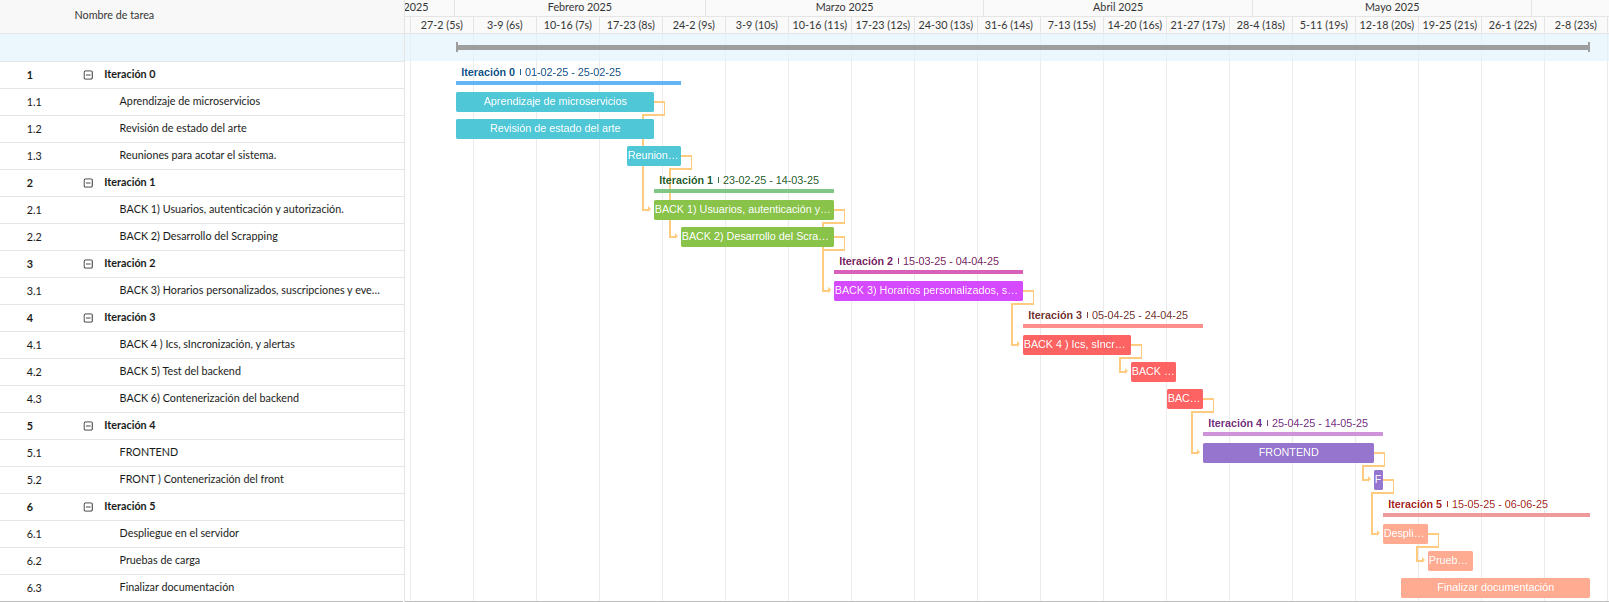
\includegraphics[width=1\textwidth]{figures/04_gantt.png}
    \caption{Gantt del proyecto.} 
    \label{gantt}
\end{figure}

El cronograma del proyecto se ha dividido en 5 sprints, cada uno con una duración de 3 semanas. Como se muestra en la figura \ref{gantt}, cada sprint ha tenido un conjunto de tareas generales a realizar, que se han ido completando a lo largo del desarrollo.

\begin{enumerate}
    \item \textbf{Sprint 0:} En este sprint se paraleliza por un lado el aprendizaje técnico acerca de microservicios, docker y el framework de desarrollo backend Spring Boot, a la vez que se acota el sistema y se recaban los requisitos iniciales del sistema.
    \item \textbf{Sprint 1:} En este sprint se comienza el desarrollo del backend implementando los servicios relativos a los usuarios, y la autenticación y autorización basadas en las credenciales de la UGR junto al servicio de mensajería (notificaciones). Además se implementa el scrapping de la we de ``Grados UGR'' para obtener los horarios de los grados.
    \item \textbf{Sprint 2:} En este sprint se continúa el backend implementando las funcionalidades relativas a suscripciones, horarios personalizados y creación de eventos.
    \item \textbf{Sprint 3:} En este sprint se desarrolla la parte del backend relacionada con generación de archivos ics, sincronización con sistemas de calendarios externos y alertas. Además se realizan tests y la contenerización del sistema.
    \item \textbf{Sprint 4:} En este sprint se desarrolla el frontend del sistema, implementando la interfaz de usuario y la comunicación con el backend.
    \item \textbf{Sprint 5:} En este último sprint se realiza el despliegue en el servidor de la UGR, se realizan pruebas de carga y se finaliza el proyecto para su entrega. Además se añade la funcionalidad extra de búsqueda de suscripciones por nombre de profesor, de modo que podemos suscribirnos directamente a los grupos de aasignaturas que imparte este.
\end{enumerate}

En todos los sprints se realizarán además tareas de documentación y pruebas, además del seguimiento y registro de horas dedicadas a cada tarea.

\section{Metodología de desarrollo}
Para la gestión y desarrollo del proyecto, se ha optado por la metodología ágil \hyperlink{scrum}{Scrum}. Esta metodología se caracteriza por su enfoque iterativo e incremental, permitiendo una adaptación flexible a los cambios y una entrega temprana de valor.

\subsection{Roles y Responsabilidades en este Proyecto}

Dada la naturaleza individual de este proyecto, los roles tradicionales de Scrum se han adaptado de la siguiente manera:

\begin{itemize}
    \item \textbf{Equipo de Desarrollo y Scrum Master:} El autor de este TFG ha asumido ambos roles. Esto implica la responsabilidad de llevar a cabo el desarrollo del software, así como de facilitar el proceso Scrum, asegurando que se sigan las prácticas y principios de la metodología. Se ha encargado de la planificación, ejecución y revisión de cada sprint, así como de la identificación y resolución de impedimentos.
    \item \textbf{Product Owner:} El rol de Product Owner ha sido desempeñado tanto por el director del TFG, D. Juan Luis Jiménez Laredo, como por el autor del sistema. En esta función, ambos han sido los responsables de definir la visión del producto, priorizar el Backlog del Producto y asegurar que el desarrollo se alinee con las necesidades y expectativas del proyecto. Los dos participaron activamente en la definición de los requisitos y en la validación de los incrementos de software.
\end{itemize}

\subsection{Proceso Scrum Implementado}

El proceso Scrum se ha implementado siguiendo los siguientes pasos clave:

\begin{itemize}
    \item \textbf{\hyperlink{backlog}{Backlog} del Producto:} Se ha definido un Backlog del Producto inicial, compuesto por las funcionalidades y tareas necesarias para completar el TFG.
    \item \textbf{Sprints:} El desarrollo se ha dividido en 5 sprints de duración 3 semanas cada uno. Cada sprint ha tenido como objetivo la entrega de un incremento de software funcional y potencialmente entregable.
    \item \textbf{Planificación del Sprint:} Al inicio de cada sprint, se ha llevado a cabo una reunión de planificación en la que, junto con el Product Owner, se han seleccionado los elementos del Backlog del Producto que se abordarían durante el sprint. Se han estimado las tareas y se ha definido el Sprint Backlog.
    \item \textbf{Desarrollo del Sprint:} Durante el sprint, el autor ha trabajado en el desarrollo de las tareas asignadas, siguiendo las prácticas de desarrollo y asegurando la calidad del código.
    \item \textbf{Reunión Diaria (Daily Scrum):} Aunque adaptada a la naturaleza individual del proyecto, se ha realizado una reflexión diaria sobre el progreso, los impedimentos y las tareas a realizar. Esto ha permitido mantener un seguimiento constante del avance.
    \item \textbf{Revisión del Sprint (Sprint Review):} Al finalizar cada sprint, se ha llevado a cabo una revisión del sprint. Dado que el autor es también el equipo de desarrollo, esta revisión ha consistido en una \textbf{introspección personal y un análisis de los resultados del sprint}, evaluando las metas alcanzadas y el incremento de software desarrollado. Se ha realizado una autoevaluación del progreso y la calidad del trabajo.
    \item \textbf{Retrospectiva del Sprint (Sprint Retrospective):} La retrospectiva del sprint se ha realizado en colaboración con el Product Owner (D. Juan Luis Jiménez Laredo). En esta reunión, se ha analizado el sprint finalizado, identificando qué se ha hecho bien, qué se podría mejorar y qué acciones concretas se podrían implementar para el siguiente sprint. Esta colaboración ha permitido obtener una perspectiva externa y valiosa para la mejora continua del proceso.
\end{itemize}

\subsection{Justificación de la Metodología}

La elección de la metodología Scrum se justifica por las siguientes razones:

\begin{itemize}
    \item \textbf{Flexibilidad:} Permite adaptarse a los cambios en los requisitos y a los aprendizajes obtenidos durante el desarrollo. En concreto este sistema dependía en etapas tempranas de desarrollo del posible acceso a datos oficiale de la UGR, sistemas de autenticación internos, datos de matriculaciones, etc. Es por ello que la flexibilidad de Scrum ha sido clave para ajustar el plan a medida que se han ido conociendo más detalles.
    \item \textbf{Entrega Temprana de Valor:} Facilita la entrega de incrementos funcionales de software de forma regular, lo que permite obtener retroalimentación temprana y ajustar el rumbo del proyecto si es necesario.
    \item \textbf{Transparencia:} El uso de herramientas como GitHub Projects y la realización de las reuniones Scrum promueven la transparencia en el progreso del proyecto.
    \item \textbf{Adaptabilidad a un Proyecto Individual:} Aunque tradicionalmente Scrum se aplica a equipos, su estructura iterativa y adaptable se ajusta bien a un proyecto individual como un TFG, permitiendo una organización eficiente del trabajo y una gestión del tiempo efectiva.
\end{itemize}

Es importante destacar que, dada la naturaleza individual del proyecto, se ha realizado una adaptación de los roles y las ceremonias de Scrum para ajustarse a las necesidades y recursos disponibles. 
Sin embargo, se han mantenido los principios fundamentales de la metodología para asegurar una gestión eficaz del desarrollo.

\subsection{Gestión de Tareas y Seguimiento del Progreso}

Para la gestión de las tareas y el seguimiento del progreso del proyecto, se ha utilizado \textbf{GitHub Projects}. Esta herramienta ha permitido:

\begin{itemize}
    \item \textbf{Creación de un Backlog del Producto:} Se ha creado un backlog del producto en GitHub Projects, donde se han definido las historias de usuario y las tareas necesarias para el desarrollo del sistema. Este backlog ha sido la base para la planificación de los sprints y la gestión de las tareas.
    \newline\newline
    Cada tarea creada en este ha representado una historia de usuario o una tarea aparte a realizar ( reuniones, investigación, etc.). Cada tarea ha sido asignada a un sprint y se ha estimado el tiempo necesario para su realización usando la técnica de \textbf{``Planning Poker''}. Esta técnica ha permitido una estimación más precisa y consensuada entre el Product Owner y el equipo de desarrollo.
    Además cada historia de usuario conllevaba una seriie de criterios de aceptación que se han ido marcando a medida que se iban cumpliendo. 
    
    \begin{figure}[H] 
        \centering 
        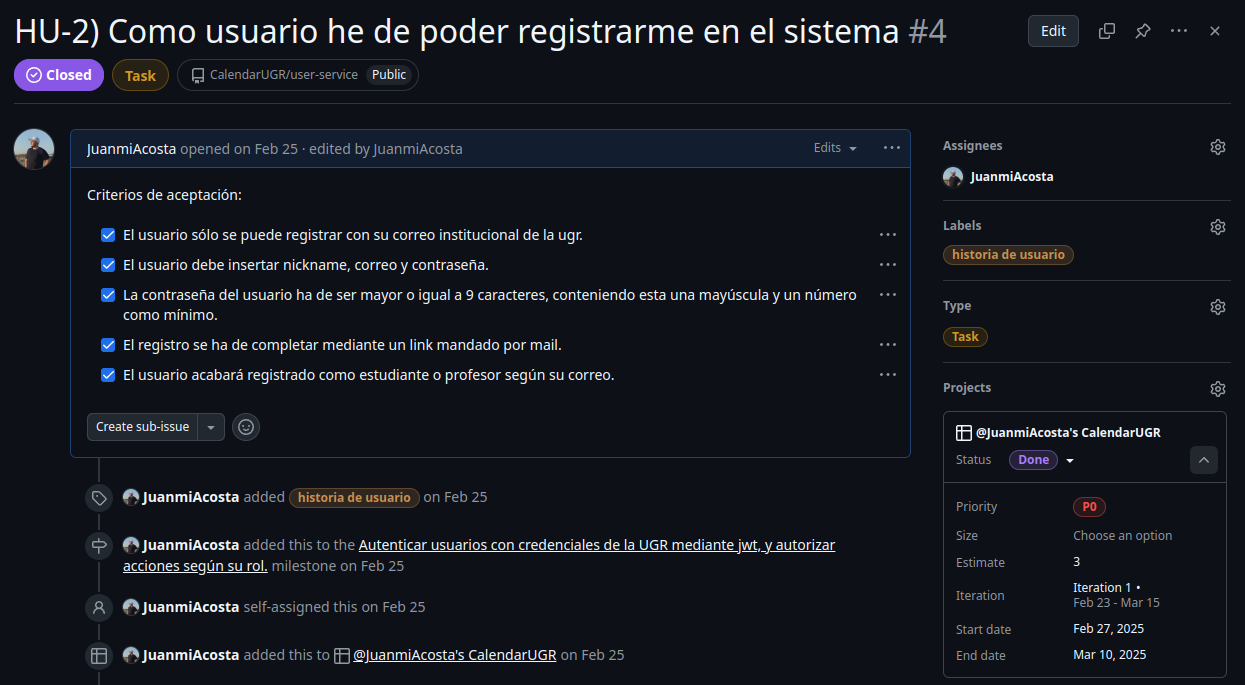
\includegraphics[width=0.9\textwidth]{figures/05_hu.png}
        \caption{Ejemplo de historia de usuario en Github Projects.} % Leyenda de la imagen
        \label{historia de usuario} % Etiqueta para referenciar la imagen
    \end{figure}

    \item \textbf{Creación de Tableros por Sprint:} Se han configurado tableros de proyecto en GitHub Projects, utilizando las funcionalidades de \textbf{``Iteraciones''} para representar cada sprint. Esto ha facilitado la visualización del trabajo en curso para cada iteración.
    \newline
    Antes del comienzo de cada sprint se revisa el product backlog, se seleccionan las tareas a realizar y se crea el tablero correspondiente poniendo todas las tareas en estado ``To do''. Además también se revisan las prioridades de estas y se cambian si el proyecto lo requiere.
    Durante el desarrollo del sprint, las tareas se van moviendo a los diferentes estados según su avance ( ``Backlog'', ``Todo'', ``In progress'', ``Testing'', ``Done'').
    
    \begin{figure}[H] 
        \centering 
        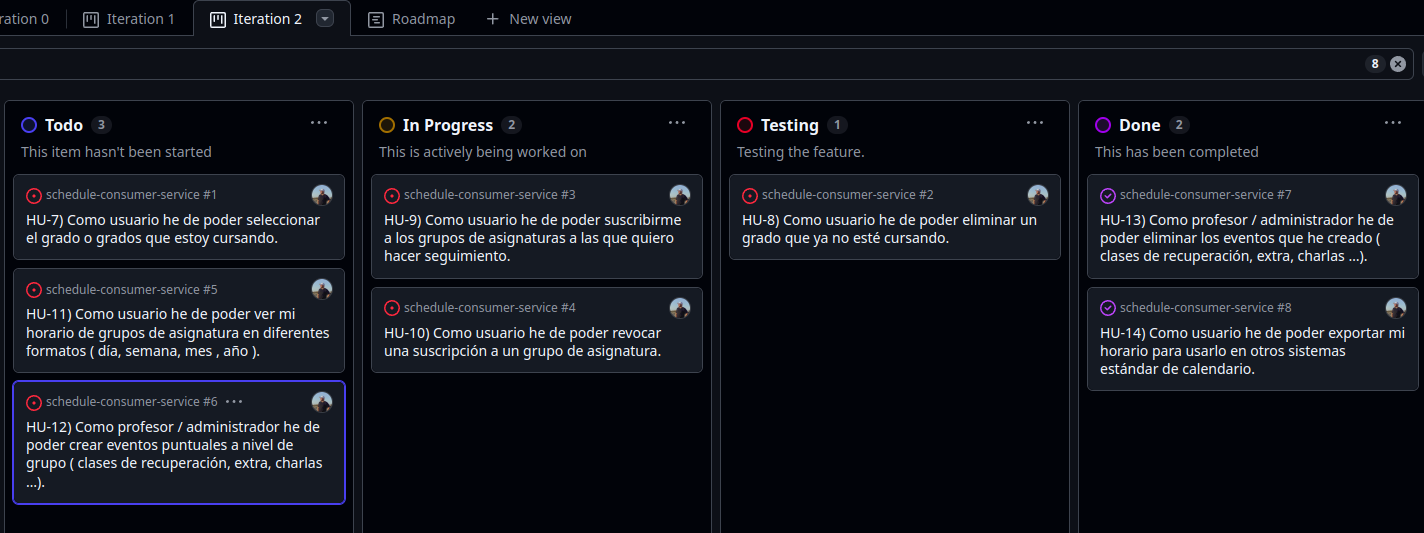
\includegraphics[width=1\textwidth]{figures/04_github_tablero.png}
        \caption{Tablero del 2º Sprint durante su desarrollo.} % Leyenda de la imagen
        \label{tablero_github} % Etiqueta para referenciar la imagen
    \end{figure}
    
    \item \textbf{Visualización de las tareas en el tiempo:} La herramienta ha permitido visualizar el progreso de las tareas en el tiempo a través de un roadmap, lo que ha facilitado la identificación de posibles retrasos y la toma de decisiones para ajustar el plan si es necesario.

    \begin{figure}[H] 
        \centering 
        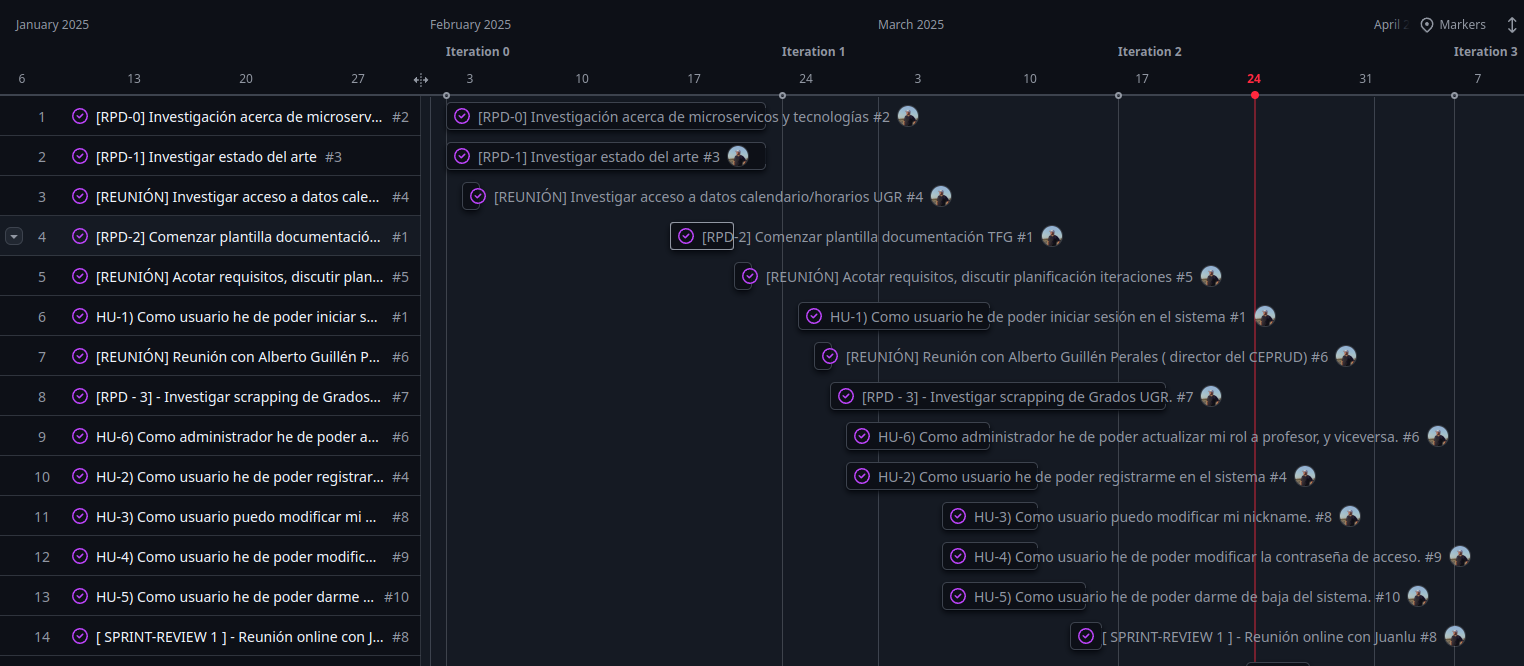
\includegraphics[width=1\textwidth]{figures/04_roadmap.png}
        \caption{Segmento del ''Roadmap'' del proyecto.} % Leyenda de la imagen
        \label{roadmap_github} % Etiqueta para referenciar la imagen
    \end{figure}
\end{itemize}

Para la gestión del tiempo dedicado a cada tarea, se ha utilizado la funcionalidad de \textbf{``Time Tracking''} Clockify. Esta funcionalidad permite registrar el tiempo dedicado a cada tarea y generar informes sobre el progreso del proyecto. Además, se ha utilizado la técnica de \textbf{``Pomodoro''} para gestionar el tiempo de trabajo, lo que ha permitido mantener un enfoque constante y evitar la fatiga.
\newline\newline
\textbf{Clockify}\cite{clockify} es una herramienta de seguimiento del tiempo que permite registrar el tiempo dedicado a cada tarea y generar informes sobre el progreso del proyecto. Esta herramienta ha sido utilizada para llevar un control detallado del tiempo invertido en cada tarea, lo que ha facilitado la gestión del tiempo y la identificación de posibles retrasos.
Además nos facilita un total de horas dedicadas al desarrollo del proyecto, por lo que facilita demostrar el esfuerzo realizado en el mismo.

\begin{figure}[H] 
    \centering 
    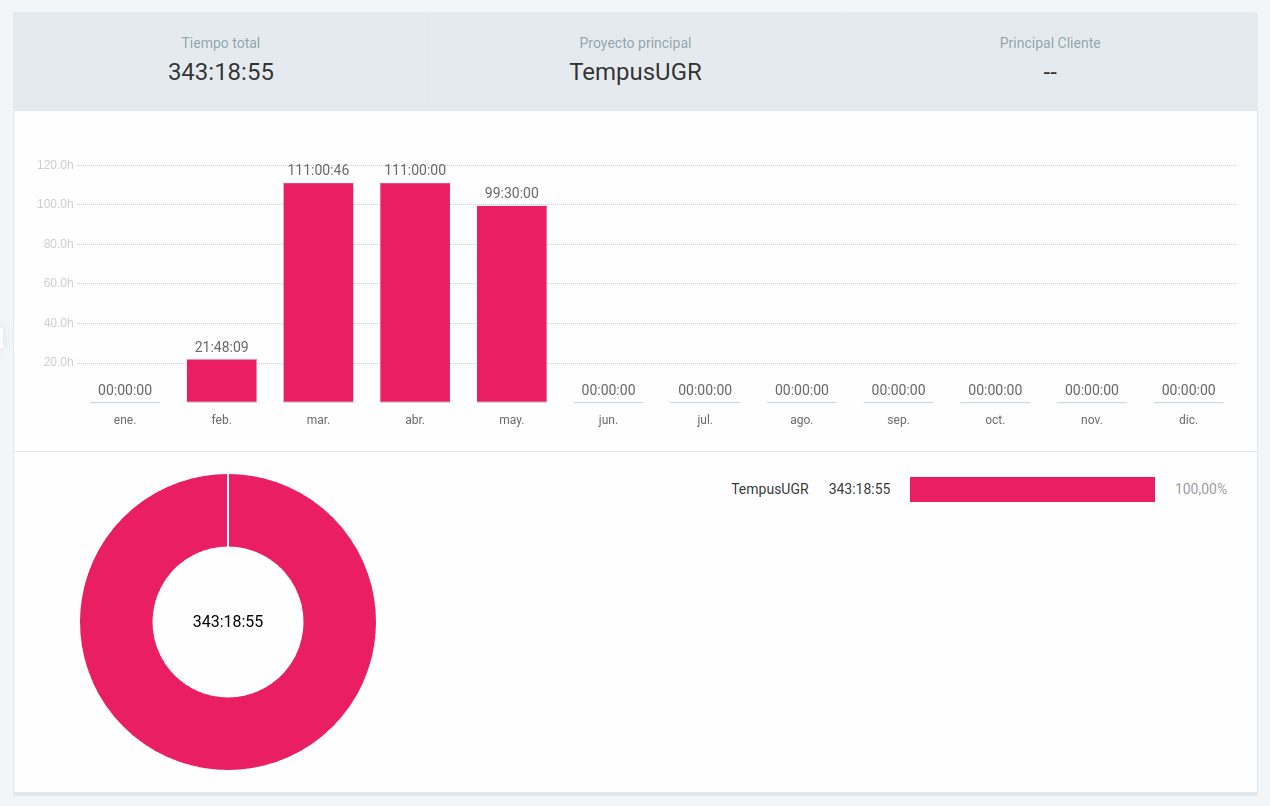
\includegraphics[width=0.8\textwidth]{figures/05_clockify.png}
    \caption{Segmento del ''Roadmap'' del proyecto.} % Leyenda de la imagen
    \label{clockify} % Etiqueta para referenciar la imagen
\end{figure}

Este resumen de horas son las correspondientes a los sprints del 1 al 5, e incluye las horas dedicadas a tareas de desarrollo, investigación, reuniones y documentación. En total, y sumando 28.5 horas del curso de microservicos, 5 horas de investigación inicial, y otras 5 horas de reuniones en la iteración 0, se han dedicado un total de 376.5 horas al desarrollo del proyecto.

\section{Gestión de riesgos}

En todo proyecto de desarrollo de software, es fundamental identificar y gestionar los riesgos que pueden afectar al éxito del mismo. A continuación se presentan los principales riesgos identificados en este proyecto, junto con las estrategias de mitigación implementadas:

\begin{itemize}
    \item \textbf{Riesgo de cambios en los requisitos:} Dado que desde la el principio del proyecto se trabajó con incertidumbre respecto a la información de la que se podía disponer ( información de los horarios académicos, matriculaciones del alumnado, autenticación institucional ...) y la posibilidad de acceso a estos datos, se ha optado por una metodología ágil (Scrum) que permite adaptarse a los cambios en los requisitos de manera flexible. Además, se ha mantenido una comunicación constante con el Product Owner para ajustar el backlog del producto según sea necesario.
    \newline\newline Además se ha ido ajustando y equilibrando las tareas a realizar entre los sprints, de manera que se realizaban las tareas más prioritarias que eran más difícil que cambiaran con el paso del tiempo, y se dejó para el final ciertas tareas que no estaban tan definidas.

    \item \textbf{Riesgo de problemas técnicos:} Durante el desarrollo del proyecto, se han presentado diversos problemas técnicos relacionados con la implementación de microservicios, la integración de APIs y la contenerización del sistema. Para mitigar este riesgo, se ha realizado una investigación exhaustiva sobre las tecnologías utilizadas y se han seguido buenas prácticas de desarrollo. Además, se ha mantenido una documentación detallada del proceso de desarrollo para facilitar la resolución de problemas.
    \newline\newline En caso de que se presentaran problemas técnicos que no pudieran resolverse, se ha mantenido una comunicación constante con el director del TFG para buscar soluciones y alternativas.

    \item \textbf{Imposibilidad de cumplir con los plazos establecidos:} Dada la naturaleza individual del proyecto, existe el riesgo de no poder cumplir con los plazos establecidos en el cronograma. Para mitigar este riesgo, se ha realizado una planificación detallada de las tareas y se ha mantenido un seguimiento constante del progreso. Además, se han establecido hitos intermedios para evaluar el avance del proyecto y realizar ajustes si es necesario.
    
    \item \textbf{Acceso a la información necesaria}: Durante el desarrollo del proyecto, se ha dependido de la disponibilidad de información externa (horarios académicos, autenticación institucional, etc.). Para mitigar este riesgo, se ha mantenido una comunicación constante con el Product Owner y se han explorado alternativas en caso de que no se pudiera acceder a la información necesaria. Además, se ha optado por implementar un sistema de scrapping para obtener los horarios académicos de la web de ``Grados UGR'' como una solución alternativa, y se ha mantenido persistencia de los datos en la base de datos del sistema para evitar depender de la disponibilidad de la web.
\end{itemize}

\section{Estimación de costes}

\subsection{Costes de personal}

Tal y como se describe el apartados anteriores, el desarrollo del proyecto ha constado de 376.5 horas de trabajo, distribuidas en los diferentes sprints y tareas a realizar.
\newline\newline
El coste de personal se ha estimado en función del coste por hora del personal involucrado en el proyecto. En este caso, considerando que según la plataforma Glassdoor \cite{webGlassdoor} un desarrollador fullstack junior cobra en torno a 23.062 € al año, y que traduciendo a cobro por hora son en torno a 11 euros/hora, se ha estimado un coste de personal de 4.141.5 euros ( 376.5 horas * 11 euros/hora).

\subsection{Costes de suministros}

\subsubsection{Durante el desarrollo}

Durante el desarrollo del proyecto, se han utilizado servicios que han generado costes asociados. A continuación se detallan los principales costes de suministros:






    \chapter{Diseño del sistema: Arquitectura, tecnologías y decisiones clave}\label{cap:disenio}

Este capítulo profundiza en el \textbf{diseño del sistema}, abarcando desde su \textbf{arquitectura general} y la \textbf{elección de tecnologías y frameworks}, hasta el \textbf{diseño de la base de datos} y la \textbf{API}. También se detallan el \textbf{diseño de la interfaz de usuario (UI)} y la \textbf{experiencia de usuario (UX)}, elementos cruciales para garantizar una aplicación intuitiva y accesible.

\section{Decisiones de diseño y arquitectura: Cimientos del sistema}

Esta sección es fundamental, ya que explica la \textbf{arquitectura general del sistema}, definiendo cómo se organizan sus componentes y cómo interactúan. La elección arquitectónica es decisiva para la \textbf{escalabilidad, mantenibilidad y robustez} de la aplicación a largo plazo.

\subsection{El Backend como pilar central}

Desde el inicio del proyecto, el \textbf{diseño del backend} se conceptualizó como la \textbf{piedra angular del sistema}. Dada la complejidad de la lógica de negocio y la gestión de datos, se priorizó una \textbf{infraestructura robusta y escalable} capaz de manejar eficientemente las operaciones principales. Esta decisión asegura la \textbf{estabilidad, rendimiento y seguridad}, independientemente de la interfaz de usuario.

\subsection{Arquitectura de Microservicios: Flexibilidad y escalabilidad}

Para cumplir con los exigentes requisitos de escalabilidad, flexibilidad y mantenibilidad a largo plazo, se optó por una \textbf{arquitectura basada en microservicios} para el backend. Esta elección permite descomponer la aplicación en \textbf{componentes independientes y débilmente acoplados}, cada uno con una funcionalidad de negocio específica.


\begin{table}[H]
    \centering
    \label{tab:monolitico_vs_microservicios_checks}
    \begin{tabular}{|p{4cm}|c|c|}
        \hline
        \textbf{Característica} & \textbf{Arquitectura Monolítica} & \textbf{Arquitectura de Microservicios} \\
        \hline
        \textbf{Velocidad de Desarrollo Inicial} & \checkmark\checkmark\checkmark & \checkmark \\
        \hline
        \textbf{Escalabilidad Independiente} & & \checkmark\checkmark\checkmark \\
        \hline
        \textbf{Mantenibilidad a Largo Plazo} & \checkmark & \checkmark\checkmark\checkmark \\
        \hline
        \textbf{Flexibilidad Tecnológica (Políglota)} & & \checkmark\checkmark\checkmark \\
        \hline
        \textbf{Resiliencia (Aislamiento de Fallos)} & \checkmark & \checkmark\checkmark\checkmark \\
        \hline
        \textbf{Despliegues Rápidos y Frecuentes} & \checkmark & \checkmark\checkmark\checkmark \\
        \hline
        \textbf{Complejidad Operacional} & \checkmark\checkmark\checkmark & \checkmark \\
        \hline
        \textbf{Coste Inicial de Infraestructura} & \checkmark\checkmark\checkmark & \checkmark \\
        \hline
        \textbf{Adaptabilidad a Cambios} & \checkmark & \checkmark\checkmark\checkmark \\
        \hline
        \textbf{Independencia de Equipos} & \checkmark & \checkmark\checkmark\checkmark \\
        \hline
    \end{tabular}
    \caption{Comparativa: Arquitectura Monolítica vs. Microservicios}
\end{table}

Comparada con una arquitectura monolítica, los microservicios ofrecen ventajas significativas. Mientras que un monolito puede ser más sencillo de implementar inicialmente, su mantenimiento y escalabilidad eficiente se complican a medida que la aplicación crece. Los microservicios, en cambio, fomentan una mayor \textbf{modularidad y reutilización}, facilitando el \textbf{desarrollo ágil y la integración continua}. Cada microservicio puede ser \textbf{desarrollado, desplegado y escalado de forma independiente}, lo que agiliza la implementación de nuevas funcionalidades y la adaptación a cambios en los requisitos.

\subsection{Separación Backend-Frontend: Comunicación vía API REST}

Una decisión arquitectónica fundamental, coherente con los microservicios, es la \textbf{completa separación entre el backend y el frontend}. Esto implica que el backend funciona como una entidad autónoma, sin conocimiento directo de la presentación al usuario. Esta independencia ofrece ventajas esenciales:

\begin{itemize}
    \item \textbf{Flexibilidad de Desarrollo:} Permite que equipos de frontend y backend trabajen en paralelo con distintas tecnologías, acelerando el ciclo de desarrollo.
    \item \textbf{Reusabilidad de Servicios:} Un mismo backend puede soportar múltiples interfaces de usuario (web, móvil), evitando la duplicidad de lógica de negocio.
    \item \textbf{Escalabilidad Horizontal Independiente:} Facilita el escalado individual de cada componente (frontend o backend) según la demanda, optimizando los recursos.
    \item \textbf{Mantenibilidad Mejorada:} Cambios en una capa (ej. refactorización del frontend) no afectan directamente a la otra, reduciendo riesgos y simplificando el mantenimiento.
    \item \textbf{Seguridad Robusta:} Permite implementar medidas de seguridad específicas y más robustas para cada componente, especialmente en el backend, que maneja datos sensibles.
\end{itemize}

La comunicación exclusiva entre el backend y el frontend se realiza mediante una \textbf{API REST (Representational State Transfer)}~\ref{fig:rest_architecture}. La elección de REST se basa en su \textbf{simplicidad, naturaleza sin estado y amplia adopción}, lo que facilita la integración e interoperabilidad. La API REST define un conjunto de \textit{endpoints} y utiliza un formato estandarizado, generalmente \textbf{JSON (JavaScript Object Notation)}, para el intercambio de datos.

\begin{figure}[H]
    \centering
    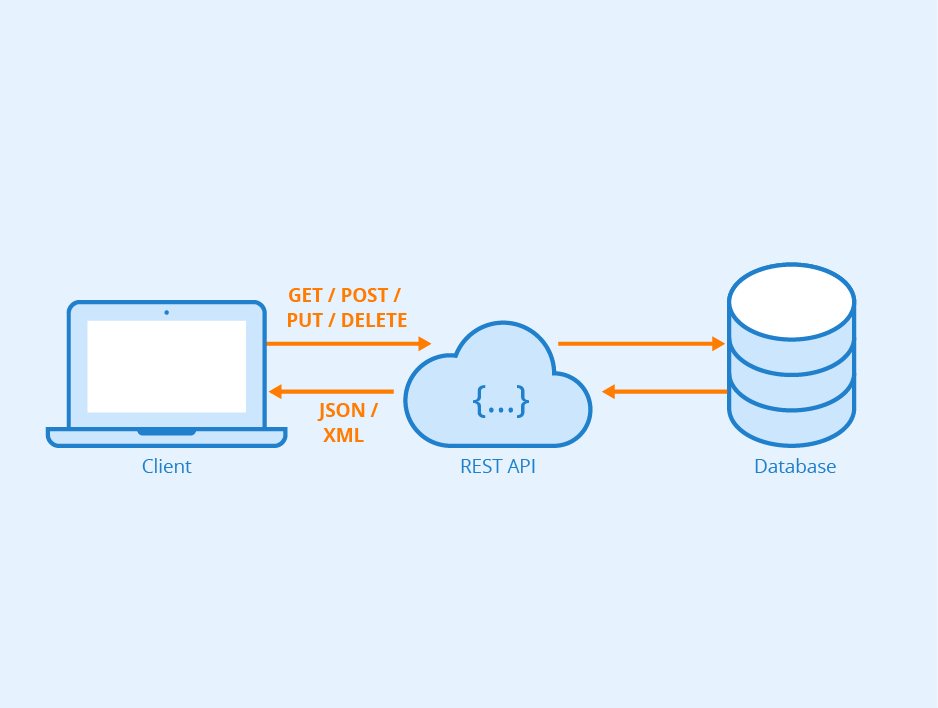
\includegraphics[width=0.8\textwidth, trim=0cm 2cm 0cm 2cm, clip]{figures/06_rest.png}
    \caption{Comunicación Backend-Frontend a través de API REST}
    \label{fig:rest_architecture}
\end{figure}

\section{Backend: Diseño y tecnologías clave}

Una vez definidos los requisitos del sistema, se procedió a diseñar el \textbf{backend} de la aplicación, siguiendo la arquitectura de microservicios, donde cada servicio gestiona una funcionalidad específica.

\subsection{Servicios del Backend identificados}

Los servicios identificados para cumplir con los requisitos del sistema son:
\begin{itemize}
    \item \textbf{Servicio de Autenticación y Autorización (Auth Service):} Gestiona el acceso, registro, inicio de sesión y permisos de usuarios.
    \item \textbf{Servicio de Gestión de Usuarios (User Service):} Responsable de la creación, actualización y eliminación de perfiles de usuario.
    \item \textbf{Servicio de Gestión de Horarios y Calendario (Schedule Consumer Service):} Obtiene y administra el horario académico desde el sistema de la UGR.
    \item \textbf{Servicio de Notificaciones (Mail Service):} Envía notificaciones a los usuarios (creación de eventos, registro completado, reseteo de contraseña, etc.).
    \item \textbf{Servicio de Matriculaciones (Academic Subscription Service):} Gestiona las matriculaciones de usuarios en asignaturas y grupos, actualiza el horario personalizado y crea eventos adicionales.
\end{itemize}

Cada servicio se implementa como una aplicación independiente para una mayor flexibilidad y escalabilidad. La comunicación entre ellos se realiza tanto vía \textbf{API REST} como mediante \textbf{eventos a través de RabbitMQ}, lo que crea una arquitectura más robusta y desacoplada. Un \textbf{API Gateway} actúa como punto de entrada para todas las solicitudes del frontend, enrutándolas, gestionando la autenticación/autorización y aportando una capa adicional de seguridad.

\subsection{Tecnologías y Frameworks del Backend}

Para el desarrollo del backend, se eligió el stack tecnológico de \textbf{Java con Spring Boot}, que ofrece ventajas significativas para microservicios:

\begin{itemize}
    \item \textbf{Spring Boot:} Facilita la creación de aplicaciones Java independientes y productivas con mínima configuración.
    \item \textbf{Spring Security:} Proporciona un marco completo para una autenticación y autorización robustas.
    \item \textbf{Spring Data JPA:} Simplifica el acceso a bases de datos relacionales mediante JPA.
    \item \textbf{Spring Cloud:} Ofrece herramientas para construir aplicaciones distribuidas (descubrimiento de servicios, configuración centralizada, gestión de circuitos).
\end{itemize}

Spring Framework es una tecnología líder en Java, con un vasto ecosistema de herramientas y bibliotecas que facilitan la creación de aplicaciones robustas y escalables. La elección de Java como lenguaje de programación capitaliza un lenguaje maduro, ampliamente adoptado, con una gran comunidad, un ecosistema rico y compatibilidad con diversas plataformas y sistemas operativos, además de su velocidad de ejecución \cite{speed_comparison} en comparación con otros lenguajes usados en backend, reflejado en la figura~\ref{fig:programming_languages_speed}.

\begin{figure}[H]
    \centering
    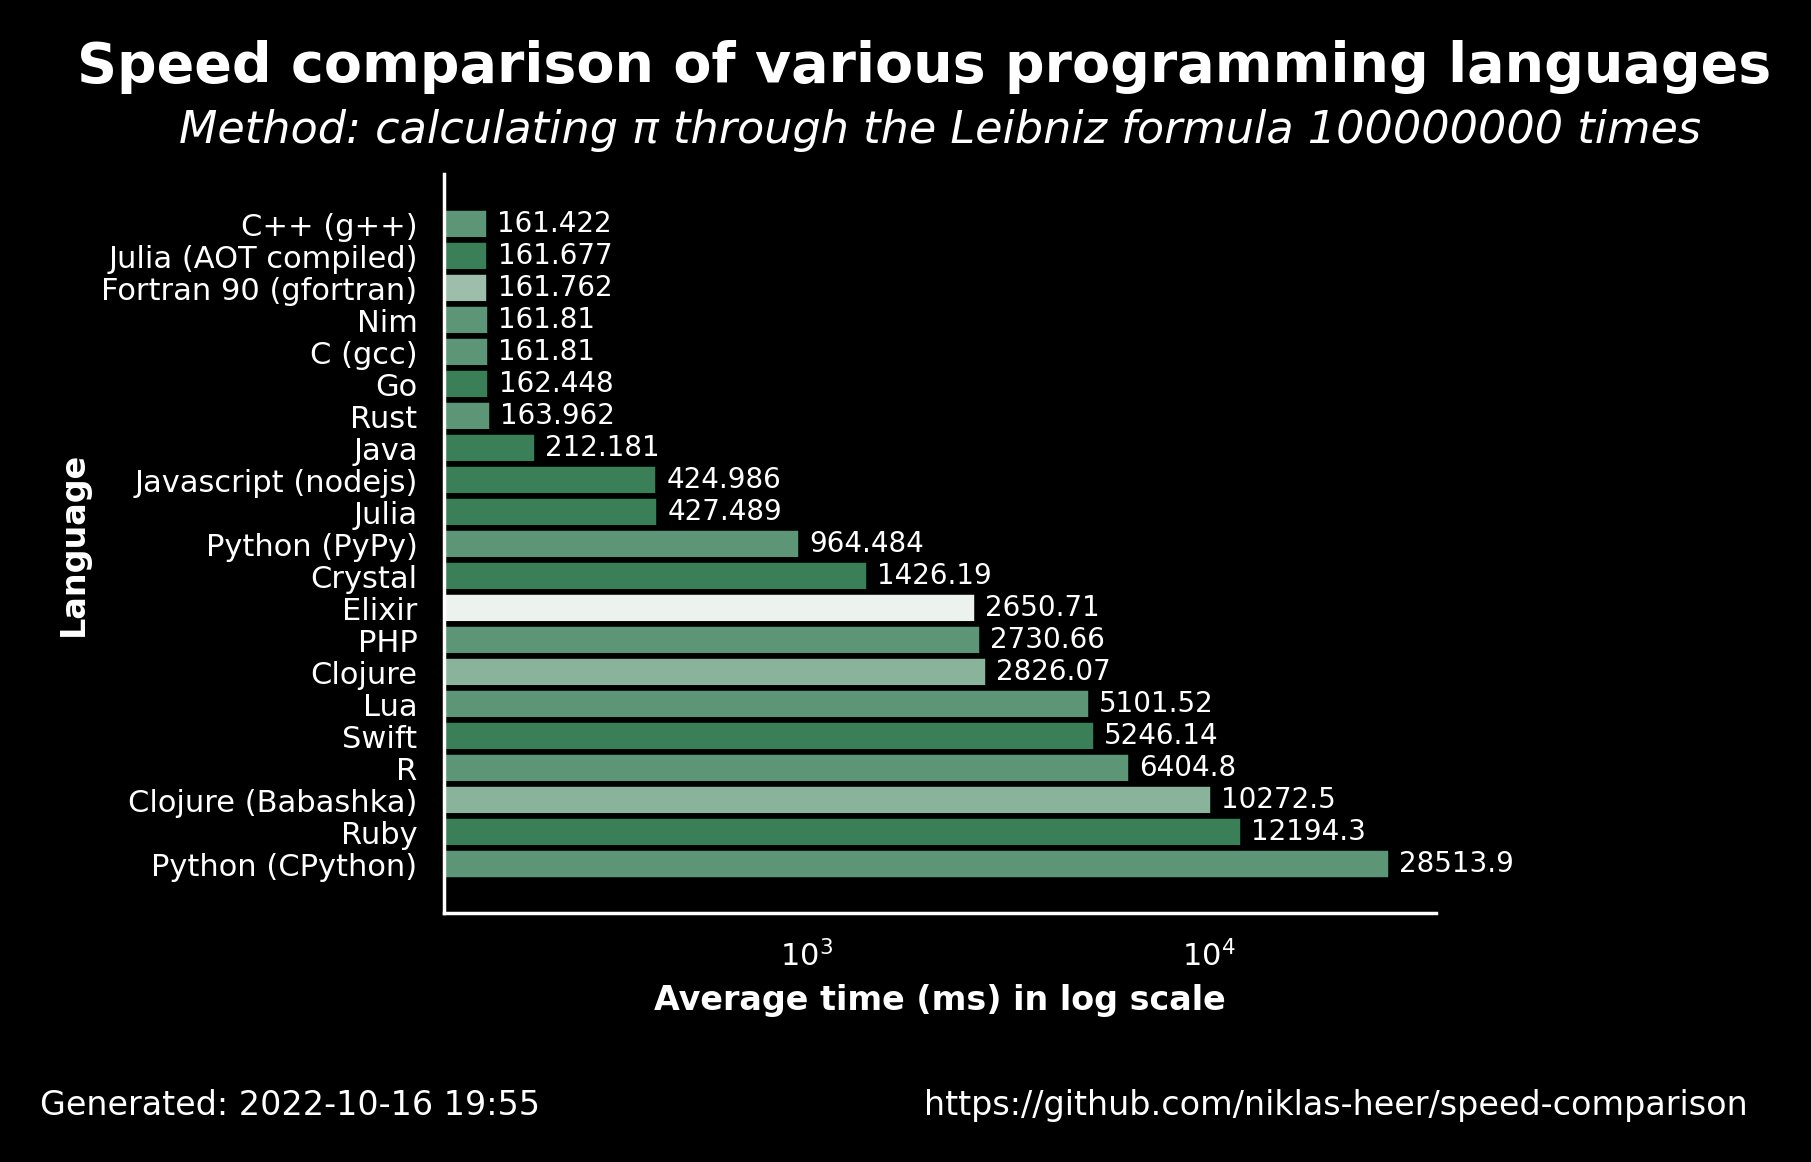
\includegraphics[width=0.9\textwidth]{figures/06_comp.png}
    \caption{Comparativa de velocidades entre lenguajes de programación}
    \label{fig:programming_languages_speed}
\end{figure}

Para el descubrimiento de servicios en esta arquitectura de microservicios, se integró \textbf{Eureka}, que permite a los servicios registrarse y descubrirse entre sí en la red. Sus ventajas incluyen:
\begin{itemize}
    \item \textbf{Descubrimiento de Servicios:} Facilita la comunicación y el enrutamiento de solicitudes entre microservicios.
    \item \textbf{Escalabilidad:} Permite añadir o eliminar instancias de servicios sin reconfiguración manual.
    \item \textbf{Resiliencia:} Ofrece mecanismos para manejar fallos de servicios, manteniendo la aplicación funcional.
    \item \textbf{Configuración Centralizada:} Simplifica la administración y el despliegue al centralizar la configuración de los servicios.
\end{itemize}

Como base de datos relacional para ``User Service'' y ``Schedule Consumer Service'' se optó por \textbf{MySQL}, un sistema de gestión de bases de datos ampliamente utilizado y confiable, que ofrece robustez, escalabilidad y un sólido soporte para transacciones. MySQL es ideal para aplicaciones que requieren integridad referencial y consultas complejas, lo que lo convierte en una excelente opción para manejar los datos de usuarios y horarios académicos.

La comunicación asíncrona y desacoplada entre servicios se logra mediante \textbf{RabbitMQ}, un sistema de mensajería ampliamente utilizado que proporciona alta disponibilidad, escalabilidad y fiabilidad en la entrega de mensajes, siendo una excelente elección para la arquitectura de microservicios. Se eligió RabbitMQ sobre alternativas como Kafka o ActiveMQ por su simplicidad, facilidad de uso, amplia adopción y compatibilidad.

Finalmente, \textbf{Docker} se seleccionó para la \textbf{contenedorización de los servicios}, permitiendo una fácil implementación y escalabilidad. Docker proporciona un entorno aislado y reproducible para cada servicio, simplificando el despliegue en diferentes entornos (desarrollo, pruebas, producción) y mejorando la portabilidad.

Tras la selección de tecnologías y la definición de las interacciones entre los servicios, se establece la siguiente arquitectura general del backend en la figura~\ref{fig:backend_architecture}:

\begin{figure}[H]
    \centering
    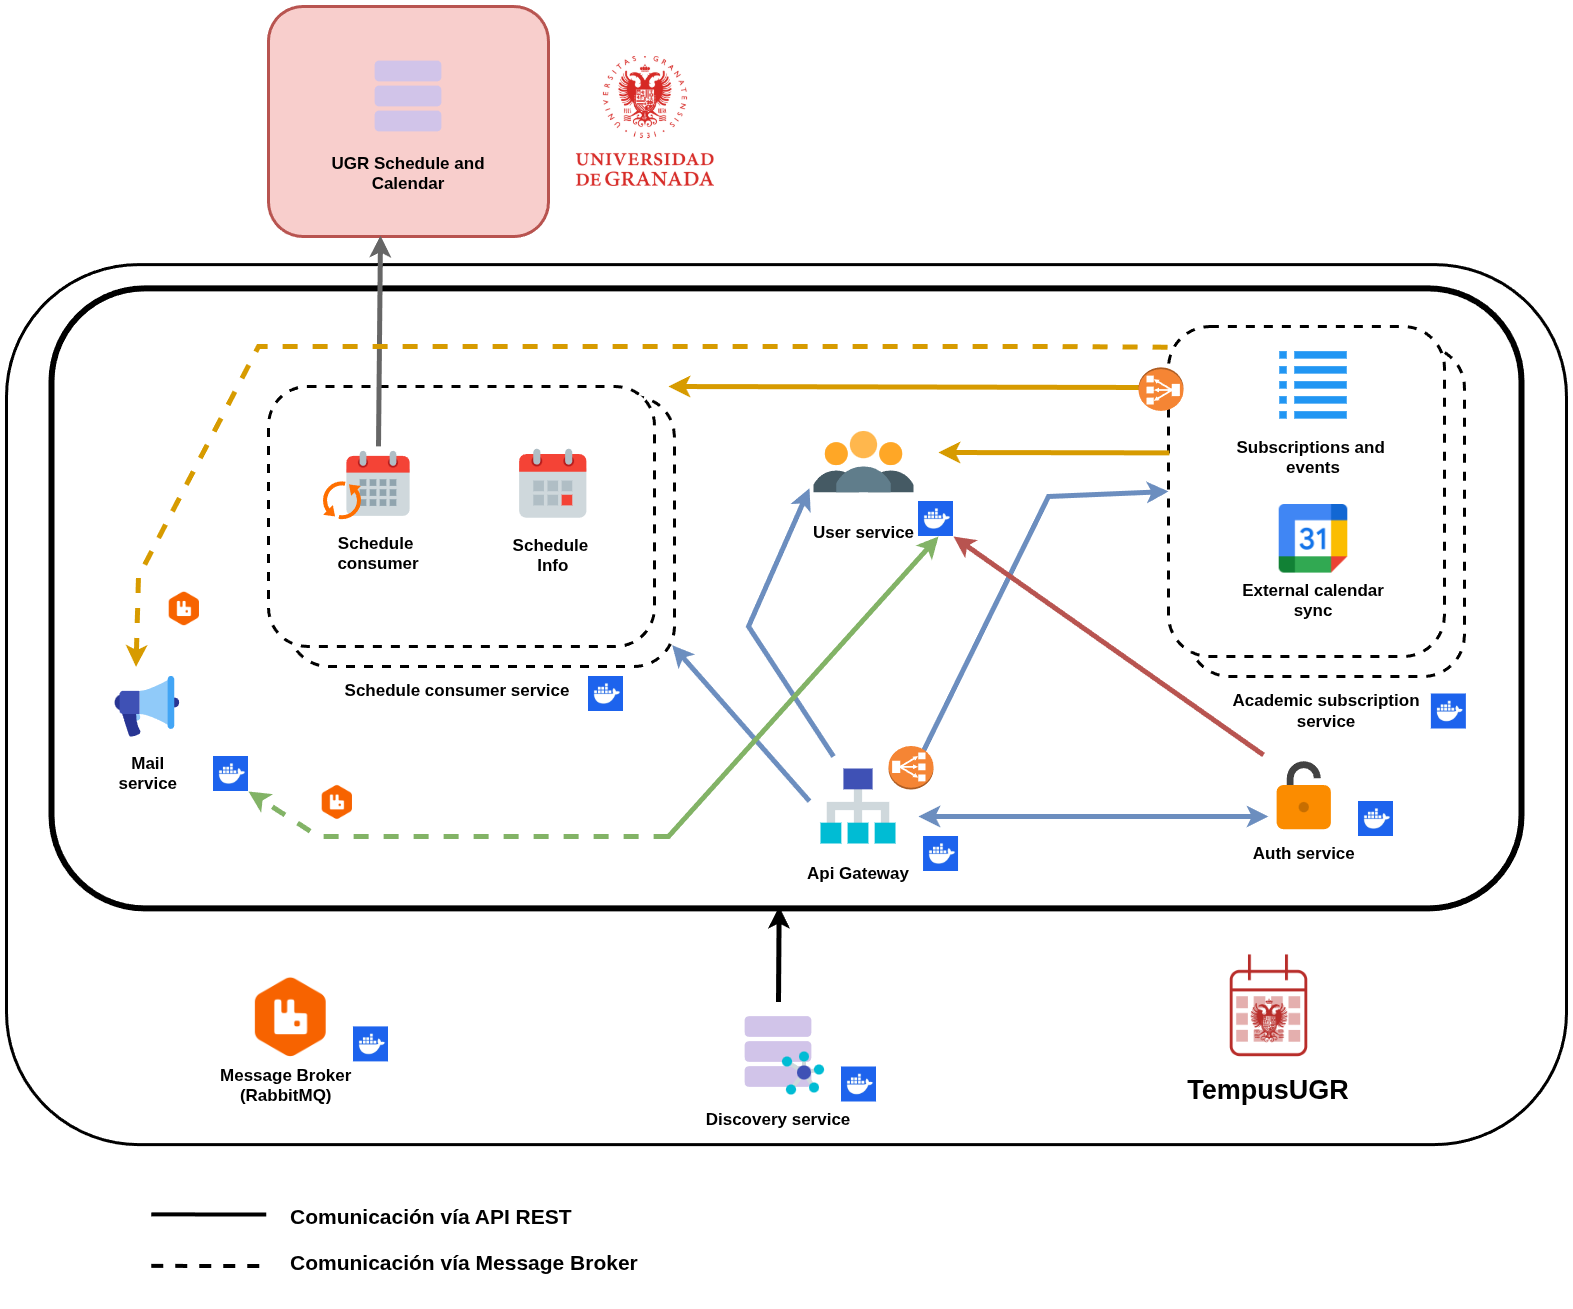
\includegraphics[width=1\textwidth]{figures/06_arq.png}
    \caption{Arquitectura general del Backend}
    \label{fig:backend_architecture}
\end{figure}

\subsubsection{Comunicaciones entre servicios}

Como se observa en el diagrama, las comunicaciones se distinguen por dos tipos principales:

\begin{itemize}
    \item \textbf{Comunicación vía API REST (Líneas Sólidas Negras y de Colores):}
    Este es el método principal para las interacciones síncronas, donde un servicio realiza una solicitud directa a otro y espera una respuesta inmediata. El \textbf{API Gateway} actúa como el punto de entrada para todas las solicitudes externas (provenientes de \texttt{TempusUGR}) y las enruta a los servicios correspondientes.
    \begin{itemize}
        \item \textbf{API Gateway $\leftrightarrow$ Auth Service:} El \textbf{API Gateway} se comunica con el \textbf{Auth Service} para gestionar la autenticación y autorización de los usuarios en cada solicitud entrante, asegurando que solo usuarios válidos y con permisos adecuados accedan a los recursos del sistema.
        \item \textbf{API Gateway $\leftrightarrow$ User Service:} Las solicitudes relacionadas con la gestión de usuarios (ej., creación, consulta, modificación de perfiles) son enrutadas desde el \textbf{API Gateway} al \textbf{User Service}.
        \item \textbf{API Gateway $\leftrightarrow$ Academic Subscription Service:} Las peticiones para gestionar suscripciones académicas, eventos personalizados y la sincronización con sistemas de calendario externos (ej., Google Calendar) se dirigen desde el \textbf{API Gateway} al \textbf{Academic Subscription Service}.
        \item \textbf{API Gateway $\leftrightarrow$ Schedule Consumer Service:} Las solicitudes para obtener información sobre horarios académicos (ej., buscar horarios de titulaciones, asignaturas) son enrutadas desde el \textbf{API Gateway} al \textbf{Schedule Consumer Service}.
        \item \textbf{Academic Subscription Service $\leftrightarrow$ User Service:} El \textbf{Academic Subscription Service} necesita comunicarse con el \textbf{User Service} para obtener información detallada de los usuarios, como sus identificadores o datos de perfil, cuando gestiona las suscripciones o eventos vinculados a ellos.
        \item \textbf{Academic Subscription Service $\leftrightarrow$ Schedule Consumer Service:} El \textbf{Academic Subscription Service} interactúa con el \textbf{Schedule Consumer Service} para obtener la información de las asignaturas matriculadas por los usuarios, como parte del proceso de construcción de sus horarios personalizados o la validación de suscripciones.
    \end{itemize}

    \item \textbf{Comunicación vía Message Broker (RabbitMQ - Líneas Discontinuas):}
    Para la comunicación asíncrona y el desacoplamiento entre servicios, se utiliza un \textbf{Message Broker (RabbitMQ)}. Este patrón es ideal para notificaciones, procesamiento en segundo plano y cuando un servicio necesita informar a otros sin esperar una respuesta inmediata.
    \begin{itemize}
        \item \textbf{Academic Subscription Service $\rightarrow$ Message Broker $\rightarrow$ Mail Service:} Cuando se producen eventos significativos en el \textbf{Academic Subscription Service} (ej., creación de una nueva suscripción, adición de un evento personalizado), este publica un mensaje en el Message Broker. El \textbf{Mail Service} consume estos mensajes para enviar notificaciones por correo electrónico a los usuarios implicados de forma asíncrona.
        \item \textbf{User Service $\rightarrow$ Message Broker $\rightarrow$ Mail Service:} De manera similar, cuando se realizan acciones relacionadas con el perfil de usuario en el \textbf{User Service} (ej., registro de un nuevo usuario, reseteo de contraseña), este publica mensajes en el Message Broker. El \textbf{Mail Service} los consume para enviar comunicaciones relevantes a los usuarios, como correos de bienvenida o confirmaciones.
    \end{itemize}
\end{itemize}

Además de estos mecanismos de comunicación explícitos, es importante destacar el papel del \textbf{Discovery Service (Eureka)}. Aunque no se muestra directamente en el flujo de datos del diagrama, es fundamental para que los microservicios puedan encontrarse y comunicarse entre sí de manera dinámica y resiliente, sin necesidad de direcciones IP o puertos codificados rígidamente.

Esta combinación de comunicación síncrona (API REST a través de API Gateway) y asíncrona (RabbitMQ) permite construir una arquitectura \textbf{robusta, escalable y mantenible}, donde los servicios pueden evolucionar de forma independiente y reaccionar a los eventos del sistema de manera eficiente y desacoplada.

\subsubsection{Obtención de horarios académicos}

El \textbf{Servicio de Horarios y Calendario (Schedule Consumer Service)} es el encargado principal de recolectar la información de horarios académicos. Para ello, se emplea una técnica de \textbf{web scraping} dirigida a la web oficial de grados de la Universidad de Granada (UGR). Este proceso consiste en la extracción automatizada de datos estructurados desde páginas web.

El flujo de obtención de horarios sigue los siguientes pasos:
\begin{enumerate}
    \item \textbf{Identificación de URLs:} El servicio está configurado con las URLs de las páginas web de grados de la UGR que contienen la información de los horarios.
    \item \textbf{Raspado de datos:} Se utiliza un algoritmo de web scraping para navegar por estas páginas, identificar los elementos HTML que contienen la información relevante (ej., tablas de horarios, nombres de asignaturas, grupos, profesores, aulas y fechas) y extraerlos de forma programática.
    \item \textbf{Procesamiento y Normalización:} Los datos extraídos, que inicialmente pueden estar en un formato inconsistente o no estructurado, son procesados y normalizados para ajustarse al modelo de datos definido en la base de datos del \textbf{Schedule Consumer Service} (entidades \texttt{Grade}, \texttt{Subject}, \texttt{Subject\_group}, \texttt{Class\_info}). Este paso es crucial para asegurar la coherencia y la integridad de la información.
    \item \textbf{Almacenamiento:} Una vez normalizados, los datos se persisten en la base de datos \textbf{MySQL} asociada al servicio.
\end{enumerate}

Esta estrategia de web scraping permite mantener la base de datos de horarios académicos actualizada con la información publicada por la UGR, garantizando que el sistema TempusUGR opere con los datos más recientes y precisos para la gestión de horarios y matriculaciones.

\subsubsection{Balanceo de Carga}

Como se refleja en la arquitectura, el sistema se ha preparado para levantar varias instancias de los servicios ``Academic Subscription Service'' y ``Schedule Consumer Service''. Esto permite distribuir la carga de trabajo entre múltiples instancias, mejorando la capacidad de respuesta y la disponibilidad del sistema. El balanceo de carga se gestiona a través del \textbf{API Gateway} y \textbf{Academic Subscription Service}, que enrutan las solicitudes entrantes a la instancia adecuada del servicio, basándose en criterios como la disponibilidad, la carga actual o el tipo de solicitud.
\newline\newline
EL algoritmo de balanceo de carga utilizado es el \textbf{Round Robin}, que distribuye las solicitudes entrantes de manera equitativa entre todas las instancias disponibles. Este enfoque es simple y efectivo, especialmente en escenarios donde las instancias tienen capacidades similares y se espera una carga uniforme.

\subsection{Modelado de la base de datos}

Una vez definidos los requisitos de información del sistema, y los sistemas de gestión de bases de datos a usar en cada servicio, se procedió a diseñar el modelo de datos~\ref{fig:user_service_er} para cada uno de los servicios del backend. A continuación se muestran los diagramas de entidad-relación (ER) para cada uno de estos:

\begin{figure}[H]
    \centering
    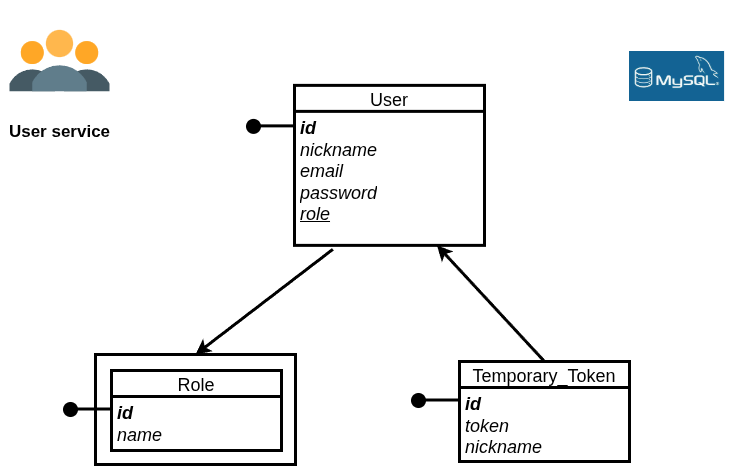
\includegraphics[width=0.7\textwidth]{figures/06_user_db.png}
    \caption{Modelo de datos del Servicio de Usuarios}
    \label{fig:user_service_er}
\end{figure}

A continuación, se detalla la estructura y propósito de cada entidad:

\begin{itemize}
    \item \textbf{Entidad User:}
    Esta entidad representa a los usuarios del sistema y es el núcleo del servicio. Almacena la información esencial para la identificación y autenticación.
    \begin{itemize}
        \item \textbf{id}: Clave primaria única para cada usuario.
        \item \textbf{nickname}: Nombre de usuario único, utilizado para la identificación en el sistema.
        \item \textbf{email}: Dirección de correo electrónico del usuario, también única y utilizada para comunicaciones y recuperación de cuenta.
        \item \textbf{password}: Contraseña del usuario, almacenada de forma segura (normalmente como un hash).
        \item \textbf{role}: Hace referencia al rol del usuario, estableciendo una relación con la entidad \textbf{Role}.
    \end{itemize}

    \item \textbf{Entidad Role:}
    Define los distintos roles o perfiles que un usuario puede tener dentro del sistema, lo que permite implementar un control de acceso basado en roles (RBAC).
    \begin{itemize}
        \item \textbf{id}: Clave primaria única para cada rol.
        \item \textbf{name}: Nombre del rol (\texttt{ROLE\_INACTIVE}, \texttt{ROLE\_STUDENT}, \texttt{ROLE\_TEACHER}, \texttt{ROLE\_ADMIN}).
    \end{itemize}
    La relación entre \textbf{User} y \textbf{Role} es de uno a muchos (un rol puede ser asignado a múltiples usuarios), o de muchos a muchos si un usuario pudiera tener varios roles (aunque el diagrama sugiere una relación de uno a muchos a través del campo \texttt{role} en \textbf{User}). Para mayor claridad en el futuro, se podría especificar el tipo de relación.

    \item \textbf{Entidad Temporary\_Token:}
    Esta entidad se utiliza para gestionar tokens de un solo uso, comúnmente empleados para procesos como la recuperación de contraseña o la verificación de correo electrónico.
    \begin{itemize}
        \item \textbf{id}: Clave primaria única para cada token temporal.
        \item \textbf{token}: El valor único del token generado.
        \item \textbf{nickname}: Hace referencia al \textbf{nickname} del usuario al que está asociado el token, estableciendo una relación directa con la entidad \textbf{User}.
    \end{itemize}
    Esta relación implica que cada token temporal está asociado a un usuario específico.
\end{itemize}

Este diseño de base de datos~\ref{fig:schedule_service_er} proporciona una estructura sólida para el \textbf{Servicio de Gestión de Usuarios}, permitiendo una gestión eficiente y segura de la información de los usuarios, sus permisos y los mecanismos de autenticación adicionales.

\begin{figure}[H]
    \centering
    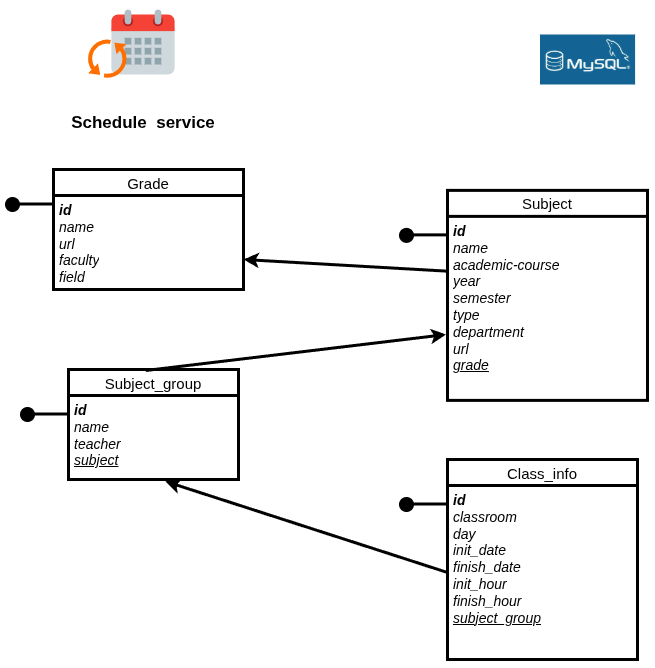
\includegraphics[width=0.7\textwidth]{figures/06_calendar_db.png}
    \caption{Modelo de datos del Servicio de Horarios y Calendario}
    \label{fig:schedule_service_er}
\end{figure}

A continuación, se describen las entidades y sus relaciones:

\begin{itemize}
    \item \textbf{Entidad Grade (Grado):}
    Representa las diferentes titulaciones académicas de las que se obtienen los horarios.
    \begin{itemize}
        \item \textbf{id}: Clave primaria única para cada titulación.
        \item \textbf{name}: Nombre completo de la titulación (ej., "Grado en Ingeniería Informática").
        \item \textbf{url}: URL o identificador del recurso externo de donde se obtienen los datos de la titulación.
        \item \textbf{faculty}: Facultad a la que pertenece la titulación.
        \item \textbf{field}: Área de conocimiento o campo de estudio de la titulación.
    \end{itemize}

    \item \textbf{Entidad Subject (Asignatura):}
    Contiene la información de las asignaturas que forman parte de las titulaciones.
    \begin{itemize}
        \item \textbf{id}: Clave primaria única para cada asignatura.
        \item \textbf{name}: Nombre de la asignatura.
        \item \textbf{academic-course}: Curso académico al que pertenece la asignatura.
        \item \textbf{year}: Año del plan de estudios en el que se imparte la asignatura.
        \item \textbf{semester}: Semestre en el que se imparte la asignatura.
        \item \textbf{type}: Tipo de asignatura (ej., ``Obligatoria'', ``Optativa'').
        \item \textbf{department}: Departamento responsable de la asignatura.
        \item \textbf{url}: URL o identificador del recurso externo de donde se obtienen los datos de la asignatura.
        \item \textbf{grade}: Clave foránea que referencia a la entidad \textbf{Grade}, indicando a qué titulación pertenece la asignatura (relación uno a muchos: una titulación tiene muchas asignaturas).
    \end{itemize}

    \item \textbf{Entidad Subject\_group (Grupo de Asignatura):}
    Representa los diferentes grupos en los que se divide una asignatura.
    \begin{itemize}
        \item \textbf{id}: Clave primaria única para cada grupo de asignatura.
        \item \textbf{name}: Nombre o identificador del grupo (ej., "Grupo 1", "Grupo A").
        \item \textbf{teacher}: Profesor o profesores asignados a este grupo.
        \item \textbf{subject}: Clave foránea que referencia a la entidad \textbf{Subject}, indicando a qué asignatura pertenece este grupo (relación uno a muchos: una asignatura tiene muchos grupos).
    \end{itemize}

    \item \textbf{Entidad Class\_info (Información de Clase):}
    Almacena los detalles específicos de cada sesión de clase para un grupo de asignatura.
    \begin{itemize}
        \item \textbf{id}: Clave primaria única para cada entrada de clase.
        \item \textbf{classroom}: Aula o lugar donde se imparte la clase.
        \item \textbf{day}: Día de la semana en que se imparte la clase.
        \item \textbf{init\_date}: Fecha de inicio de la clase o del período de clases.
        \item \textbf{finish\_date}: Fecha de finalización de la clase o del período de clases.
        \item \textbf{init\_hour}: Hora de inicio de la clase.
        \item \textbf{finish\_hour}: Hora de finalización de la clase.
        \item \textbf{subject\_group}: Clave foránea que referencia a la entidad \textbf{Subject\_group}, indicando a qué grupo de asignatura pertenece esta clase (relación uno a muchos: un grupo puede tener muchas clases).
    \end{itemize}
\end{itemize}

Este esquema de base de datos~\ref{fig:academic_subscription_service_er} permite al \textbf{Servicio de Horarios y Calendario} organizar y gestionar de manera eficiente toda la información académica necesaria para la composición de los horarios de los usuarios.

\begin{figure}[H]
    \centering
    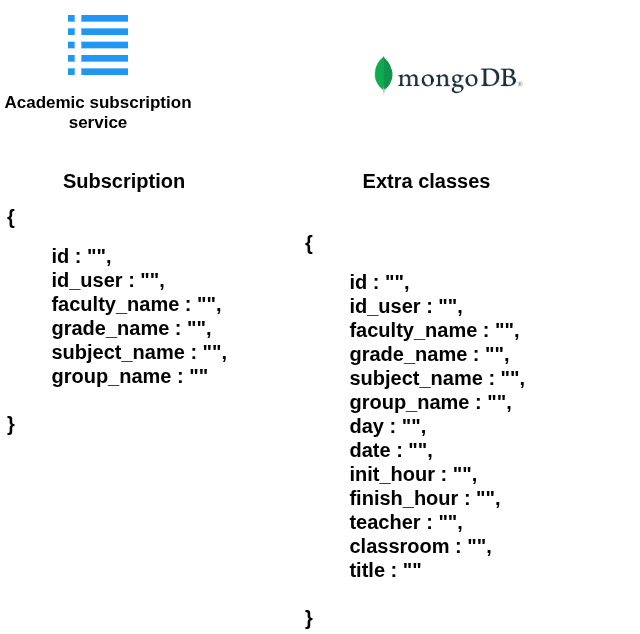
\includegraphics[width=0.7\textwidth, trim=0cm 0cm 2.5cm 0cm, clip]{figures/06_sub_db.png}
    \caption{Modelo de datos del Servicio de Matriculaciones}
    \label{fig:academic_subscription_service_er}
\end{figure}

A continuación, se detalla la estructura esperada de los documentos en cada colección:

\begin{itemize}
    \item \textbf{Colección Subscription:}
    Esta colección almacena las matriculaciones de los usuarios en asignaturas y grupos específicos, reflejando su horario oficial.
    \begin{itemize}
        \item \textbf{id}: Identificador único del documento de suscripción.
        \item \textbf{id\_user}: Identificador del usuario al que pertenece esta suscripción. Permite vincular la suscripción a un usuario específico.
        \item \textbf{faculty\_name}: Nombre de la facultad de la titulación asociada.
        \item \textbf{grade\_name}: Nombre de la titulación a la que se suscribe el usuario.
        \item \textbf{subject\_name}: Nombre de la asignatura a la que el usuario está matriculado.
        \item \textbf{group\_name}: Nombre del grupo de la asignatura al que el usuario está matriculado.
    \end{itemize}
    Esta estructura flexible permite registrar la información de la matriculación sin la rigidez de un esquema relacional fijo, adaptándose a posibles variaciones en los detalles académicos.

    \item \textbf{Colección Extra classes:}
    Esta colección está diseñada para almacenar clases o eventos adicionales que los usuarios puedan crear para su horario personalizado, no directamente vinculados al horario oficial.
    \begin{itemize}
        \item \textbf{id}: Identificador único del documento de clase extra.
        \item \textbf{id\_user}: Identificador del usuario que creó esta clase adicional.
        \item \textbf{faculty\_name}: Nombre de la facultad relacionada con la clase (opcional, para contexto).
        \item \textbf{grade\_name}: Nombre de la titulación relacionada (opcional, para contexto).
        \item \textbf{subject\_name}: Nombre de la asignatura (si aplica, para contexto).
        \item \textbf{group\_name}: Nombre del grupo (si aplica, para contexto).
        \item \textbf{day}: Día de la semana en que se imparte la clase extra.
        \item \textbf{date}: Fecha específica de la clase extra.
        \item \textbf{init\_hour}: Hora de inicio de la clase extra.
        \item \textbf{finish\_hour}: Hora de finalización de la clase extra.
        \item \textbf{teacher}: Nombre del profesor o ponente de la clase extra.
        \item \textbf{classroom}: Aula o lugar donde se imparte la clase extra.
        \item \textbf{title}: Título o descripción breve de la clase extra.
    \end{itemize}
    La flexibilidad de MongoDB es particularmente útil aquí, ya que los campos pueden variar entre documentos de "Extra classes" dependiendo de la naturaleza del evento.
\end{itemize}

La elección de MongoDB para estas colecciones permite una \textbf{rápida inserción y consulta de datos}, así como una \textbf{fácil adaptación a cambios en el esquema de datos} sin requerir migraciones complejas, lo que es ventajoso para la gestión dinámica de las suscripciones y eventos personalizados de los usuarios.

\subsection{Diseño de la API}

El diseño de la API del backend se basa en el principio de \textbf{REST (Representational State Transfer)}, que define un conjunto de convenciones para la creación de servicios web escalables y mantenibles. La API está estructurada en torno a recursos, cada uno representado por una URL única, y utiliza los métodos HTTP estándar para interactuar con estos recursos.
\newline\newline
Para su estandarización se ha seguido la especificación de la \textbf{RFC 7231}\cite{rfc7231}, que define el HyperText Transfer Protocol (HTTP/1.1) y sus métodos, así como las convenciones para la creación de APIs RESTful. Esta especificación proporciona un marco claro para el diseño de APIs, asegurando que sean intuitivas, predecibles y fáciles de consumir por los clientes.
\newline
Además de esta se ha revisado la \textbf{RFC 1738}\cite{rfc1738}, que define el formato de las URLs, asegurando que todas las rutas de la API sigan una estructura coherente y fácil de entender. Esto es crucial para la usabilidad de la API, ya que permite a los desarrolladores comprender rápidamente cómo interactuar con los diferentes recursos del sistema.
\newline\newline
Para hacer pruebas y documentar la API de manera efectiva, se ha utilizado \textbf{Postman}, una herramienta ampliamente adoptada en la comunidad de desarrollo para probar y documentar APIs. Postman permite a los desarrolladores enviar solicitudes HTTP a la API, inspeccionar las respuestas y crear colecciones de pruebas que pueden ser compartidas y reutilizadas. Además, facilita la generación de documentación interactiva de la API, lo que mejora la experiencia del desarrollador al integrar o consumir los servicios.

\subsubsection{Estructura de la API}

En primer lugar, y gracias al uso de un \textbf{API Gateway}, se ha definido una estructura de URL base para la API, que es la siguiente:
\begin{lstlisting}[language=Java]
http://<host>:<port>/calendarugr/v1
\end{lstlisting}
Donde ``\<host\>'' la ip del host donde se despliega la aplicación y ``\<port\>'' es el puerto en el que escucha el API Gateway. Esta estructura base permite una fácil identificación de la versión de la API y proporciona un punto de entrada común para todas las solicitudes. Además en secciones posteriores al implementar https, y al adquirir un dominio de la UGR, esta URL base se actualizará para reflejar el dominio oficial del servicio.
\begin{lstlisting}[language=Java]
https://tempus.ugr.es/calendarugr/v1
\end{lstlisting}

A partir de esta URL base, los diferentes microservicios exponen sus funcionalidades a través de rutas específicas. La API se ha estructurado lógicamente según los servicios del backend, facilitando la comprensión y el uso por parte de los clientes. A continuación, se detallan los principales grupos de endpoints.

\noindent\textbf{Nota sobre Autorización:} Todos los endpoints de la API requieren autenticación y autorización mediante JWT, con las siguientes excepciones que son de acceso público o gestionan la autenticación inicial:
\begin{itemize}
    \item \texttt{/auth/login}
    \item \texttt{/auth/refresh}
    \item \texttt{/user/register}
    \item \texttt{/user/activate}
    \item \texttt{/academic-subscription/ics} (para la descarga pública de calendarios ICS)
    \item \texttt{/academic-subscription/sync-url} (para la obtención de URLs públicas de sincronización)
    \item \texttt{/user/reset-pass-mail}
    \item \texttt{/user/reset-password} 
\end{itemize}

\paragraph{\textbf{Endpoints del Servicio de Usuarios (User Service):}}
Gestionan la administración de usuarios, roles y la recuperación de contraseñas.
\begin{itemize}
    \item \textbf{Administración de Usuarios (Admin Endpoints):}
    \begin{itemize}
        \item \textbf{POST /user/admin/register}
        \newline Descripción: Crea un usuario sin la necesidad de pasar por confirmación de cuenta (para Administrador).
        \newline Cuerpo (JSON):
\begin{lstlisting}[language=bash]
{
  "nickname": "string",
  "email": "string",
  "password": "string",
  "role": {
    "name": "string"
  },
  "notification": true
}
\end{lstlisting}

        \item \textbf{PUT /user/admin/update/\{id\}}
        \newline Descripción: Actualiza la información de un usuario por su ID (para Administrador).
        \newline Cuerpo (JSON):
\begin{lstlisting}[language=bash]
{
  "nickname": "string",
  "email": "string",
  "password": "string",
  "role": {
    "name": "string"
  },
  "notification": true
}
\end{lstlisting}

        \item \textbf{DELETE /user/admin/delete/\{id\}}
        \newline Descripción: Elimina un usuario por su ID.
    \end{itemize}
    
    \item \textbf{Gestión de Roles (Role related):}
    \begin{itemize}
        \item \textbf{POST /user/role/create}
        \newline Descripción: Crea un nuevo rol.
        \newline Cuerpo (JSON):
\begin{lstlisting}[language=bash]
{
  "name": "string"
}
\end{lstlisting}

        \item \textbf{GET /user/role/all}
        \newline Descripción: Obtiene todos los roles disponibles.

        \item \textbf{DELETE /user/role/delete}
        \newline Descripción: Borra un rol existente.
        \newline Cuerpo (JSON):
\begin{lstlisting}[language=bash]
{
  "name": "string"
}
\end{lstlisting}
    \end{itemize}
    
    \item \textbf{Recuperación de Contraseña (Password recovery):}
    \begin{itemize}
        \item \textbf{POST /user/reset-pass-mail}
        \newline Descripción: Solicita el envío de un correo electrónico para el reseteo de contraseña.
        \newline Parámetros de consulta: mail (string)
    \end{itemize}

    \item \textbf{Consulta y Gestión General de Usuarios:}
    \begin{itemize}
        \item \textbf{GET /user/all}
        \newline Descripción: Obtiene la lista completa de usuarios.

        \item \textbf{GET /user/nickname/\{nickname\}}
        \newline Descripción: Obtiene un usuario por su nickname.

        \item \textbf{GET /user/email/\{email\}}
        \newline Descripción: Obtiene un usuario por su dirección de correo electrónico.

        \item \textbf{GET /user/user-info}
        \newline Descripción: Obtiene la información del usuario asociado al token actual.

        \item \textbf{POST /user/register}
        \newline Descripción: Registra un nuevo usuario en el sistema.
        \newline Cuerpo (JSON):
\begin{lstlisting}[language=bash]
{
  "nickname": "string",
  "email": "string",
  "password": "string"
}
\end{lstlisting}

        \item \textbf{POST /user/activate}
        \newline Descripción: Activa una cuenta de usuario utilizando un token de activación.
        \newline Parámetros de consulta: token (string)

        \item \textbf{PUT /user/deactivate}
        \newline Descripción: Desactiva la cuenta del usuario actual.
        \newline Cuerpo (JSON):
\begin{lstlisting}[language=bash]
{
  "currentPassword": "string"
}
\end{lstlisting}

        \item \textbf{PUT /user/nickname}
        \newline Descripción: Actualiza el nickname del usuario actual.
        \newline Cuerpo (JSON):
\begin{lstlisting}[language=bash]
{
  "nickname": "string"
}
\end{lstlisting}

        \item \textbf{PUT /user/role}
        \newline Descripción: Cambia el rol de un usuario.

        \item \textbf{PUT /user/password}
        \newline Descripción: Actualiza la contraseña del usuario actual.
        \newline Cuerpo (JSON):
\begin{lstlisting}[language=bash]
{
  "currentPassword": "string",
  "newPassword": "string"
}
\end{lstlisting}

        \item \textbf{PUT /user/activate-notifications}
        \newline Descripción: Activa las notificaciones para el usuario actual.

        \item \textbf{PUT /user/deactivate-notifications}
        \newline Descripción: Desactiva las notificaciones para el usuario actual.

        \item \textbf{POST /user/email-list}
        \newline Descripción: Obtiene una lista de correos electrónicos de usuarios basándose en una lista de IDs.
        \newline Cuerpo (JSON):
\begin{lstlisting}[language=bash]
[
  "id1",
  "id2"
]
\end{lstlisting}
    \end{itemize}

    \item \textbf{Endpoints del Servicio de Autenticación (Auth Service):}
    Gestionan el proceso de inicio de sesión y la renovación de tokens.
    \begin{itemize}
        \item \textbf{POST /auth/login}
        \newline Descripción: Permite a un usuario iniciar sesión en el sistema.
        \newline Cuerpo (JSON):
\begin{lstlisting}[language=bash]
{
  "email": "string",
  "password": "string"
}
\end{lstlisting}

        \item \textbf{POST /auth/refresh}
        \newline Descripción: Permite renovar un token de acceso utilizando un refresh token.
        \newline Cuerpo (JSON):
\begin{lstlisting}[language=bash]
{
  "refreshToken": "string"
}
\end{lstlisting}
    \end{itemize}

    \item \textbf{Endpoints del Servicio de Correo (Mail Service):}
    Se utilizan para enviar correos electrónicos.
    \begin{itemize}
        \item \textbf{POST /email/send}
        \newline Descripción: Envía un correo electrónico.
        \newline Cuerpo (JSON):
\begin{lstlisting}[language=bash]
{
  "receiver": "string",
  "subject": "string",
  "message": "string"
}
\end{lstlisting}
    \end{itemize}

    \item \textbf{Endpoints del Servicio de Horarios (Schedule Consumer Service):}
    Proporcionan acceso a la información de horarios académicos obtenida mediante web scraping.
    \begin{itemize}
        \item \textbf{GET /schedule-consumer/classes-from-group}
        \newline Descripción: Obtiene las clases de un grupo específico de una asignatura y titulación.
        \newline Parámetros de consulta: grade (string), subject (string), group (string)

        \item \textbf{GET /schedule-consumer/grades}
        \newline Descripción: Obtiene la lista de todas las titulaciones disponibles.

        \item \textbf{GET /schedule-consumer/subjects-groups}
        \newline Descripción: Obtiene las asignaturas y grupos asociados a una titulación específica.
        \newline Parámetros de consulta: grade (string)

        \item \textbf{GET /schedule-consumer/teacher-classes}
        \newline Descripción: Obtiene las clases impartidas por un profesor, buscando por nombre parcial.
        \newline Parámetros de consulta: partialTeacherName (string)
    \end{itemize}

    \item \textbf{Endpoints del Servicio de Matriculaciones Académicas (Academic Subscription Service):}
    Permiten a los usuarios gestionar sus suscripciones a asignaturas y grupos, así como crear y gestionar eventos personalizados.
    \begin{itemize}
        \item \textbf{GET /academic-subscription/classes}
        \newline Descripción: Obtiene las clases a las que el usuario está suscrito.

        \item \textbf{GET /academic-subscription/entire-calendar}
        \newline Descripción: Obtiene el calendario completo del usuario (suscripciones y eventos extra).

        \item \textbf{GET /academic-subscription/subscriptions}
        \newline Descripción: Obtiene las suscripciones activas del usuario.

        \item \textbf{POST /academic-subscription/subscription}
        \newline Descripción: Suscribe al usuario a una asignatura y grupo específicos.
        \newline Cuerpo (JSON):
\begin{lstlisting}[language=bash]
{
  "faculty": "string",
  "grade": "string",
  "subject": "string",
  "group": "string"
}
\end{lstlisting}

        \item \textbf{POST /academic-subscription/subscription-batching}
        \newline Descripción: Permite suscribirse a múltiples asignaturas y grupos en una sola solicitud.
        \newline Cuerpo (JSON):
\begin{lstlisting}[language=bash]
[
  {
    "faculty": "string",
    "grade": "string",
    "subject": "string",
    "group": "string"
  }
]
\end{lstlisting}

        \item \textbf{GET /academic-subscription/ics}
        \newline Descripción: Permite descargar el calendario del usuario en formato ICS.

        \item \textbf{GET /academic-subscription/sync-url}
        \newline Descripción: Obtiene una URL pública para sincronizar el calendario ICS del usuario con otras aplicaciones.

        \item \textbf{DELETE /academic-subscription/subscription-grade}
        \newline Descripción: Borra todas las suscripciones de un usuario para una titulación específica.

        \item \textbf{DELETE /academic-subscription/subscription}
        \newline Descripción: Borra una suscripción específica de un usuario.

        \item \textbf{GET /academic-subscription/group-event}
        \newline Descripción: Obtiene los eventos de grupo (clases extra) creados por el usuario.

        \item \textbf{POST /academic-subscription/group-event}
        \newline Descripción: Inserta una nueva clase extra o evento de grupo para el usuario.
        \newline Cuerpo (JSON):
\begin{lstlisting}[language=bash]
{
  "classroom": "string",
  "day": "string",
  "date": "YYYY-MM-DD",
  "initHour": "HH:MM:SS",
  "finishHour": "HH:MM:SS",
  "groupName": "string",
  "subjectName": "string",
  "teacher": "string",
  "gradeName": "string",
  "facultyName": "string",
  "title": "string"
}
\end{lstlisting}

        \item \textbf{DELETE /academic-subscription/group-event}
        \newline Descripción: Borra un evento de grupo específico por su ID.

        \item \textbf{GET /academic-subscription/faculty-group-event}
        \newline Descripción: Recoge todos los eventos creados por la facultad del usuario.

        \item \textbf{POST /academic-subscription/faculty-event}
        \newline Descripción: Crea un evento a nivel de facultad.
        \newline Cuerpo (JSON):
\begin{lstlisting}[language=bash]
{
  "day": "string",
  "date": "YYYY-MM-DD",
  "initHour": "HH:MM:SS",
  "finishHour": "HH:MM:SS",
  "facultyName": "string",
  "title": "string"
}
\end{lstlisting}

        \item \textbf{DELETE /academic-subscription/faculty-event}
        \newline Descripción: Borra un evento de facultad por su ID.
    \end{itemize}
\end{itemize}

\section{Frontend: Diseño y tecnologías clave} 

El frontend de TempusUGR se ha desarrollado utilizando \textbf{Angular}, un framework de desarrollo web que permite crear aplicaciones de una sola página (SPA) de manera eficiente y escalable. Angular es conocido por su arquitectura basada en componentes, lo que facilita la reutilización de código y la separación de preocupaciones, permitiendo un desarrollo más organizado y mantenible.
\newline\newline
Se alinea con las mejores prácticas de desarrollo web moderno, incluyendo el uso de \textbf{TypeScript} como lenguaje principal, lo que proporciona tipado estático y características avanzadas de programación orientada a objetos. Esto mejora la calidad del código y facilita la detección temprana de errores durante el desarrollo.
\newline\newline
Además, Angular cuenta con un robusto sistema de inyección de dependencias, lo que permite una gestión eficiente de los servicios y componentes, mejorando la modularidad y la testabilidad de la aplicación. También incluye herramientas integradas para el manejo del enrutamiento, la gestión del estado y la comunicación con APIs RESTful, lo que simplifica el desarrollo de aplicaciones complejas.

\subsection{Diseño de la Interfaz y Experiencia del Usuario (UI/UX)}

En cuanto a la parte visual del proyecto, se tuvo en mente desde el principio tener una interfaz usable, intuitiva y accesible, de manera que se facilitara lo máximo posible el acceso a la información del horario personalizado.
\newline\newline
Para ello, se optó por un diseño minimalista, como el reflejado en el logo en la figura~\ref{fig:logo}, con una paleta de colores clara y un uso moderado de imágenes. Además se utilizó la tipografía ``Segoe UI'' por su diseño moderno con letras redondeadas y diseño limpio que se ve bien en pantallas y papel.
\newline
\begin{center}
\begin{minipage}{0.5\textwidth}
    \begin{itemize}
        \item Color primario: \#b82d2a \colorbox[HTML]{b82d2a}{\hspace{1.5em}} \vspace{0.7em}
        \item Color secundario: \#e4afae \colorbox[HTML]{e4afae}{\hspace{1.5em}} \vspace{0.7em}
        \item Color de fondo: \#f5f5f5 \colorbox[HTML]{f5f5f5}{\hspace{1.5em}} \vspace{0.7em}
        \item Color de texto: \#333333 \colorbox[HTML]{333333}{\hspace{1.5em}}
    \end{itemize}
\end{minipage}
\hfill
\begin{minipage}{0.25\textwidth}
    \centering
    \captionsetup{justification=centering}
    
\includegraphics[width=0.8\textwidth]{figures/logo.png}
    \captionof{figure}{Logo de TempusUGR}
    \label{fig:logo}
\end{minipage}
\end{center}

\newpage
El diseño de la interfaz se ha centrado en la usabilidad, asegurando que los usuarios puedan navegar fácilmente por las diferentes secciones de la aplicación. Se han implementado menús claros y botones intuitivos para facilitar la interacción con el sistema. Además, se ha prestado especial atención a la accesibilidad, siguiendo las pautas WCAG (Web Content Accessibility Guidelines) para garantizar que la aplicación sea usable por personas con discapacidades.
\newline\newline
Además se han seguido los diez principios de diseño de Jakob Nielsen\cite{nielsen10principles}, que son:
\begin{enumerate}
    \item \textbf{Visibilidad del estado del sistema:} La aplicación proporciona retroalimentación clara sobre las acciones del usuario, como confirmaciones de suscripciones o errores en la entrada de datos.
    \item \textbf{Coincidencia entre el sistema y el mundo real:} Se utilizan términos y conceptos familiares para los usuarios, evitando jerga técnica innecesaria.
    \item \textbf{Control y libertad del usuario:} Los usuarios pueden deshacer acciones fácilmente, como cancelar una suscripción o eliminar un evento.
    \item \textbf{Consistencia y estándares:} Se mantiene una terminología y diseño coherentes en toda la aplicación.
    \item \textbf{Prevención de errores:} Se implementan validaciones para evitar entradas incorrectas, como fechas inválidas o grupos inexistentes.
    \item \textbf{Reconocimiento en lugar de recuerdo:} Los menús y opciones son visibles y accesibles, reduciendo la carga cognitiva del usuario.
    \item \textbf{Flexibilidad y eficiencia de uso:} La aplicación permite a los usuarios realizar tareas comunes rápidamente mediante atajos y opciones avanzadas.
    \item \textbf{Diseño estético y minimalista:} La interfaz es limpia y sin distracciones innecesarias, enfocándose en la funcionalidad principal.
    \item \textbf{Ayuda a los usuarios a reconocer, diagnosticar y recuperarse de errores:} Se proporcionan mensajes de error claros y sugerencias para resolver problemas comunes.
    \item \textbf{Ayuda y documentación:} Se incluye una sección de ayuda accesible que explica cómo utilizar las principales funcionalidades de la aplicación.
\end{enumerate}
    \chapter{Implementación}\label{cap:implementacion}

En este capítulo se describe la implementación del proyecto, así como detalles técnicos y decisiones tomadas durante el desarrollo. Se divide en varios sprints, cada uno con sus propias tareas y objetivos.

\section{Sprint 0}

En este sprint no se comienza el desarrollo del proyecto, sino que, como se menciona en la sección \ref{cap:especificación} y \ref{cap:planificacion}, se realiza una investigación sobre las tecnologías a utilizar, y se detallan los requerimientos del sistema, y la arquitectura a implementar.
\newline\newline
Al usar Java (versión 21) como lenguaje de programación y Spring Boot (versión 3.4.4) como framework de desarrollo, se sigue un patrón similar para el desarrollo de los servicios, ya que todos comparten componentes y directorios similares.

\subsection{Estructura general de los servicios}

El código fuente de los servicios se organiza en paquetes, siguiendo una estructura común para todos los servicios. Esta estructura incluye:

\begin{itemize}
    \item \textbf{config}: Contiene la configuración del servicio, como la configuración de seguridad, bases de datos, etc.
    \item \textbf{controller}: Contiene los controladores REST que manejan las peticiones HTTP.
    \item \textbf{dto}: Contiene los objetos de transferencia de datos (DTO) utilizados para la comunicación entre el cliente y el servidor.
    \item \textbf{model}: Contiene las entidades del dominio del servicio.
    \item \textbf{repository}: Contiene las interfaces de repositorio que extienden de JPA para la persistencia de datos.
    \item \textbf{service}: Contiene la lógica de negocio del servicio.
    \item \textbf{mapper}: Contiene los mapeadores para convertir entre entidades y DTOs.
    \item \textbf{Application.java}: Clase principal que arranca el servicio.
\end{itemize}

De esta forma, se consigue una estructura clara y coherente para el desarrollo de los servicios, facilitando la comprensión y el mantenimiento del código.

Además para la configuración de estos, se utiliza un archivo de propiedades (application.properties) que permite definir las propiedades específicas del servicio, como la conexión a la base de datos, el puerto en el que se ejecuta el servicio, etc.

\section{Sprint 1}

Este primer sprint se comienza con cierta incertidumbre al no haber tenido todavía la reunión con Alberto Guillén Perales, el director del CEPRUD, por lo que no se sabe a qué información se va a tener acceso, y por tanto cómo se van a implementar ciertas funcionalidades.
\newline\newline
Sin embargo, ya que el proceso para poder hacer uso del sistema de autenticación de la UGR parece ser largo y requiere de una serie de permisos y pasos previos \cite{autenticacion_ugr}, se decide en este punto comenzar a implementar en el backend todas las funcionalidades relacionadas con la gestión de usuarios, y autenticación basadas en las credenciales de la UGR.
\newline\newline
Para conseguir esto se implementan los servicios ``User Service'', ``Auth Service'', ``Mail Service'' y el ``API Gateway''.

\subsection{User Service}

Este servicio se plantea como el encargado de gestionar los usuarios del sistema, permitiendo registrar, consultar, actualizar y eliminar usuarios. Además, se encarga de la gestión de roles y permisos, así como de la codificación de contraseñas.
\newline 
Las contraseñas se almacenan de forma segura mediante codificación (por ejemplo, \texttt{BCrypt}), y no en texto plano.
\newline\newline
Los usuarios pueden poseer los roles de \texttt{ROLE\_INACTIVE}, \texttt{ROLE\_STUDENT}, \texttt{ROLE\_TEACHER}, o \texttt{ROLE\_ADMIN}, y estos nos permiten controlar el acceso a diferentes funcionalidades del sistema.
\newline\newline
Aunque este servicio no es el encargado de la autenticación, sirve de soporte para el servicio de autenticación, proporcionando la información de los usuarios y sus roles.

\subsubsection{Integración con otros microservicios}

\begin{itemize}
  \item Es consultado por otros servicios para validar identidad o permisos de los usuarios.
  \item Envía mensajes mediante RabbitMQ para notificar el registro de usuarios y/o cambios en sus credenciales.
\end{itemize}

\subsubsection{Diagrama de clases}
Este es el primer servicio implementado, y se sigue una estructura similar en los demás servicios para mantener la coherencia en el proyecto. El patrón de diseño implementado a lo largo del desarrollo de los servicios es el \textbf{Modelo-Vista-Controlador (MVC)}, que separa la lógica de negocio, la presentación y el acceso a datos. Esta separación de responsabilidades facilita el mantenimiento y la escalabilidad del código, esto se refleja en el diagrama de clases del servicio User Service, que se muestra en la figura \ref{fig:user-service-class-diagram}.
\begin{figure}[H]
    \centering
    \makebox[\textwidth][c]{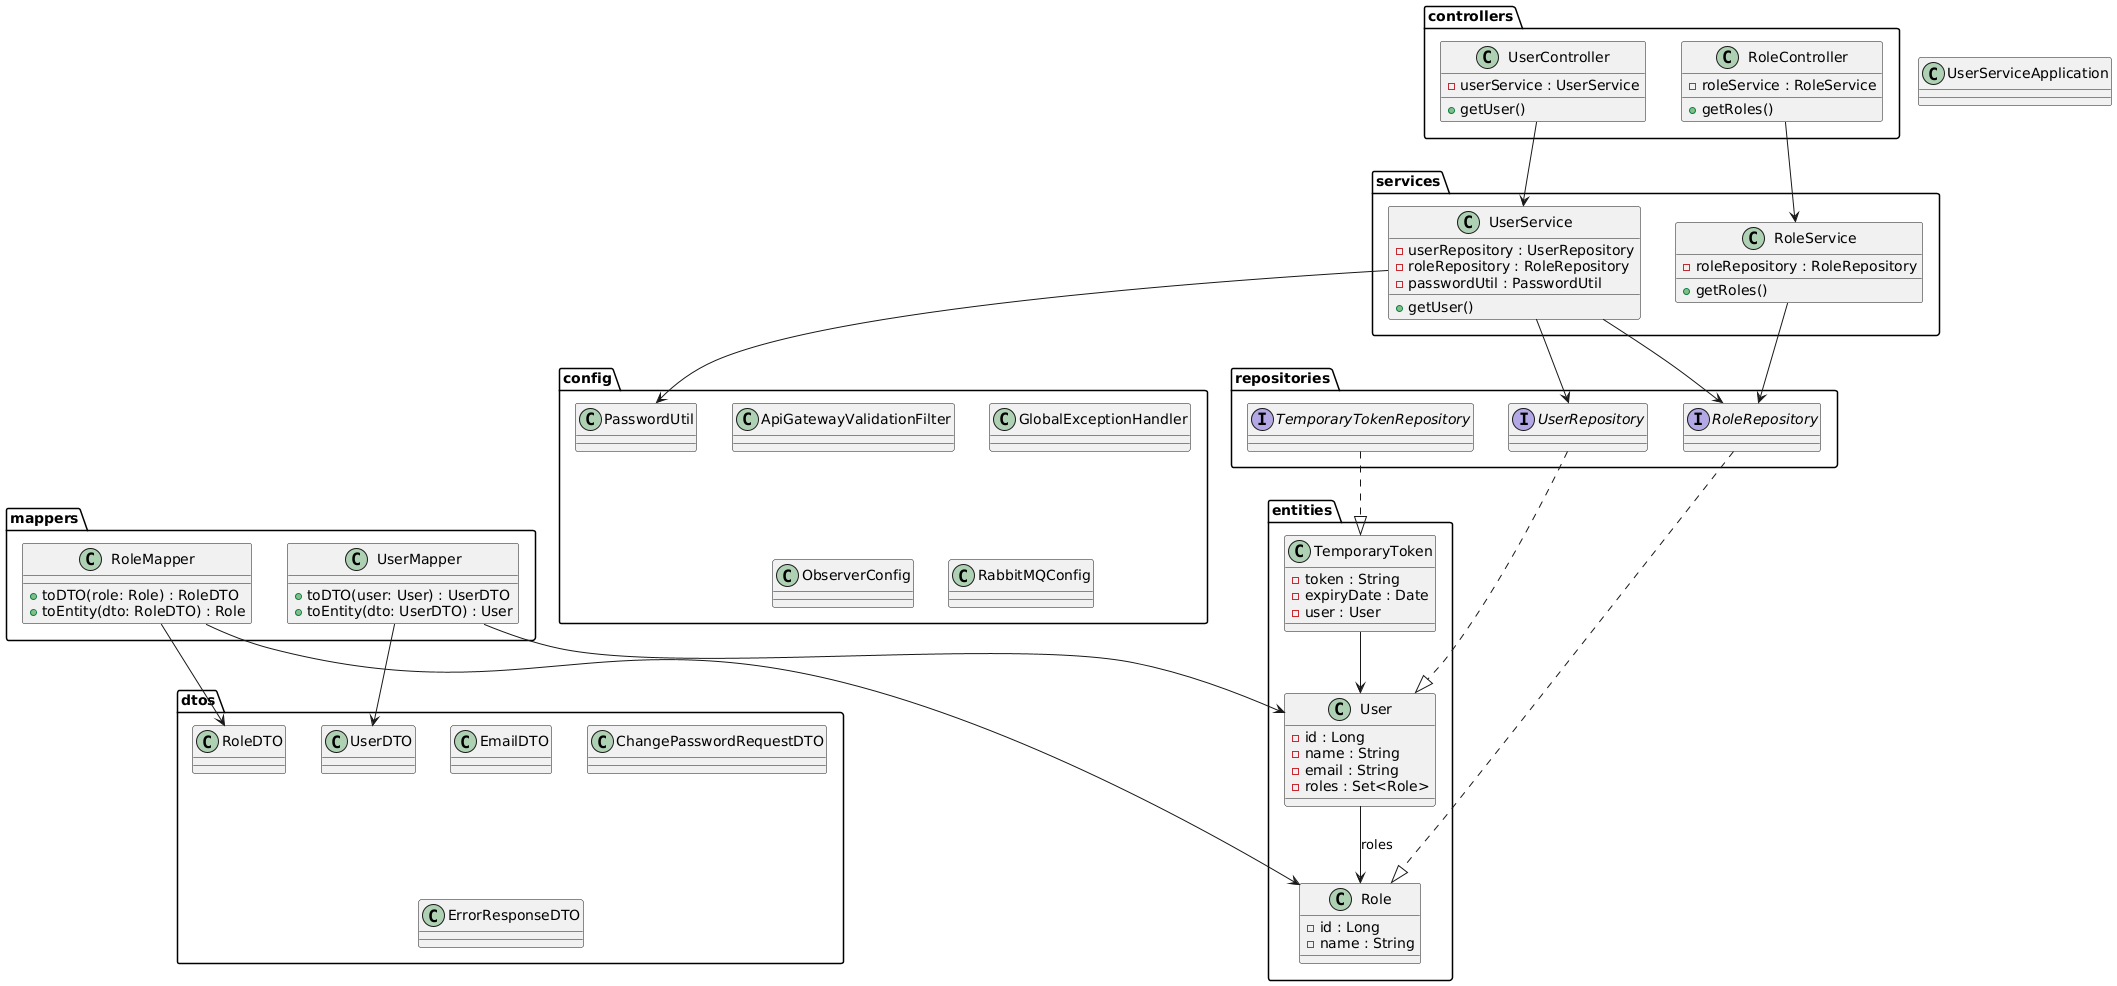
\includegraphics[width=1.2\textwidth]{figures/07_uml_user.png}}
    \caption{Diagrama de clases del servicio User Service realizado con PlantUML}
    \label{fig:user-service-class-diagram}
\end{figure}

Este diagrama representa las principales clases del servicio, incluyendo los controladores, servicios, repositorios y entidades. Cada clase tiene una responsabilidad clara y se comunica con otras clases a través de interfaces, lo que permite una fácil extensibilidad y mantenimiento del código.

\subsubsection{Interacción entre componentes}

\subsubsection*{1. Controladores (\texttt{controllers})}

\begin{itemize}
  \item \textbf{UserController} y \textbf{RoleController}: Son clases que exponen endpoints HTTP. Actúan como punto de entrada de las solicitudes del cliente.
  \item \textbf{Interacción}: Invocan métodos en los servicios correspondientes (\texttt{UserService}, \texttt{RoleService}) para obtener datos o ejecutar lógica de negocio.
\end{itemize}

\subsubsection*{2. Servicios (\texttt{services})}

\begin{itemize}
  \item \textbf{UserService}: Contiene la lógica de negocio relacionada con usuarios.
    \begin{itemize}
      \item Depende de \texttt{UserRepository} y \texttt{RoleRepository} para acceder a la base de datos.
      \item Usa \texttt{PasswordUtil} para tareas relacionadas con contraseñas (encriptación, validación, etc).
    \end{itemize}
  \item \textbf{RoleService}: Contiene lógica de negocio asociada a roles.
    \begin{itemize}
      \item Se comunica con \texttt{RoleRepository}.
    \end{itemize}
\end{itemize}

\subsubsection*{3. Repositorios (\texttt{repositories})}

\begin{itemize}
  \item \textbf{UserRepository}, \textbf{RoleRepository}, \textbf{TemporaryTokenRepository}: Son interfaces que definen operaciones CRUD (Create, Read, Update, Delete) sobre las entidades.
  \item \textbf{Interacción}: Son utilizados por los servicios para obtener o almacenar datos en la base de datos.
  Además toda la interacción con la base de datos se realiza a través de JPA, lo que permite una fácil integración y manejo de las entidades. JPA es un Objeto-Relational Mapping (ORM) que facilita la persistencia de datos en aplicaciones Java, permitiendo mapear clases Java a tablas de bases de datos relacionales.
\end{itemize}

\subsubsection*{4. Entidades (\texttt{entities})}

\begin{itemize}
  \item \textbf{User}: Representa un usuario del sistema. Tiene atributos como \texttt{id}, \texttt{name}, \texttt{email}, y una colección de \texttt{roles}.
  \item \textbf{Role}: Representa un rol o permiso dentro del sistema. Se relaciona con los usuarios.
  \item \textbf{TemporaryToken}: Usado para funcionalidades temporales como recuperación de contraseña. Contiene un \texttt{token}, una fecha de expiración y referencia al \texttt{User}.
  \item \textbf{Interacción}: Estas entidades son gestionadas por los repositorios y utilizadas en la lógica de negocio de los servicios.
\end{itemize}

\subsubsection*{5. Mapeadores (\texttt{mappers})}

\begin{itemize}
  \item \textbf{UserMapper} y \textbf{RoleMapper}: Se encargan de convertir entidades (\texttt{User}, \texttt{Role}) a sus correspondientes objetos de transferencia de datos (\texttt{UserDTO}, \texttt{RoleDTO}) y viceversa.
  \item \textbf{Interacción}: Usados por los servicios para traducir datos entre capas internas y externas.
\end{itemize}

\subsubsection*{6. DTOs (\texttt{dtos})}

\begin{itemize}
  \item \textbf{UserDTO}, \textbf{RoleDTO}, \textbf{EmailDTO}, \textbf{ChangePasswordRequestDTO}, \textbf{ErrorResponseDTO}: Representan estructuras de datos que se usan para enviar y recibir información a través de la API.
  \item \textbf{Interacción}: Son utilizados por los controladores y servicios para comunicar información de forma segura y controlada, evitando exponer entidades directamente.
\end{itemize}

\subsubsection*{7. Configuración (\texttt{config})}

\begin{itemize}
  \item \textbf{PasswordUtil}: Clase de utilidad para el manejo de contraseñas.
  \item \textbf{ApiGatewayValidationFilter}: Filtro que valida solicitudes entrantes desde el API Gateway.
  \item \textbf{GlobalExceptionHandler}: Captura y maneja excepciones globalmente.
  \item \textbf{RabbitMQConfig}, \textbf{ObserverConfig}: Configuración para mensajería y observadores (por ejemplo, eventos asincrónicos).
  \item \textbf{Interacción}: Algunas de estas clases son inyectadas en servicios (\texttt{PasswordUtil}), otras se ejecutan automáticamente (\texttt{GlobalExceptionHandler}).
\end{itemize}

\subsubsection*{8. Flujo de Interacción General}

\begin{enumerate}
  \item El cliente realiza una solicitud a través del \texttt{UserController} o \texttt{RoleController}.
  \item El controlador llama al servicio correspondiente (\texttt{UserService} o \texttt{RoleService}).
  \item El servicio accede a los repositorios para obtener datos desde las entidades.
  \item Se usan los mapeadores para convertir entidades en DTOs.
  \item El DTO es devuelto al cliente a través del controlador.
\end{enumerate}

Aunque en cada servicio se implementan diferentes funcionalidades, la estructura y la interacción entre los componentes siguen un patrón similar, lo que facilita la comprensión del código.
Para ilustrar de manera más simple lo detallado anteriormente, se muestra la figura \ref{fig:comm}, que representa la comunicación general entre los componentes del backend. 
\begin{figure}[H]
    \centering
    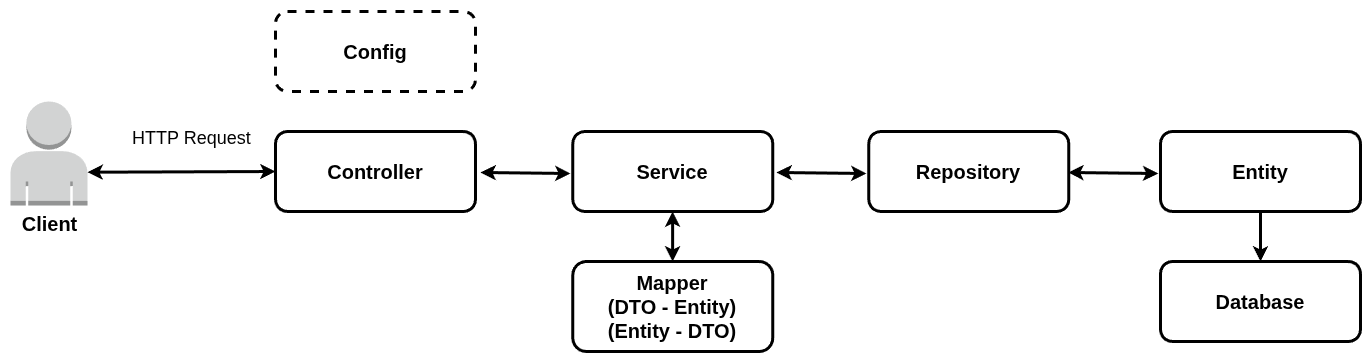
\includegraphics[width=0.95\textwidth]{figures/07_back.png}
    \caption{Comunicación general entre los componentes del backend}
    \label{fig:comm}
\end{figure}

\subsection{Mail Service}
El servicio de correo electrónico se encarga de enviar correos electrónicos a los usuarios del sistema. Este servicio es utilizado por otros servicios para enviar notificaciones, como la confirmación de registro, recuperación de contraseña, etc.

Su desarrollo combina tres tecnologías clave: \textbf{RabbitMQ}, \textbf{JavaMail} y \textbf{Thymeleaf}, permitiendo una integración fluida entre mensajería asíncrona y generación dinámica de contenido de correo.

El proceso comienza cuando otro componente del sistema necesita enviar un correo electrónico. En lugar de enviarlo directamente, publica un mensaje en una cola gestionada por \texttt{RabbitMQ}. Este servicio actúa como consumidor de esos mensajes mediante el uso de \texttt{listeners}, que reciben el contenido del mensaje en tiempo real. Esta estrategia permite desacoplar el proceso de envío de correo del resto de la lógica de negocio, mejorando la escalabilidad y la resiliencia del sistema ante posibles errores.

Una vez recibido el mensaje, el servicio extrae los datos necesarios, como la dirección de correo del destinatario, el asunto, y las variables que se inyectarán en el contenido. Para la composición del cuerpo del correo, se utiliza \texttt{Thymeleaf}, un motor de plantillas que permite construir correos HTML personalizados. Gracias a Thymeleaf, se pueden generar correos enriquecidos visualmente, dinámicos y adaptados al contexto de cada notificación, manteniendo una presentación clara y profesional.

Después de generar el contenido del correo, se utiliza la biblioteca \texttt{JavaMail} para su envío. JavaMail proporciona una API robusta y configurable que permite construir mensajes MIME, manejar los encabezados, adjuntos y establecer la conexión con el servidor SMTP. En este caso, se ha configurado el servicio para utilizar \textbf{Gmail como proveedor de correo electrónico}, lo cual requiere definir parámetros como el host SMTP de Gmail (\texttt{smtp.gmail.com}), el puerto correspondiente, y habilitar la autenticación y conexión segura mediante TLS. Esta configuración se especifica en los archivos de propiedades del servicio, lo que facilita su adaptación a distintos entornos de despliegue.

En conjunto, este microservicio representa una solución elegante y modular para el envío de correos, como el que se observa en la figura~\ref{fig:mail-service-class-diagram} en arquitecturas basadas en microservicios. Aprovecha la comunicación asincrónica de RabbitMQ, la potencia expresiva de las plantillas Thymeleaf, y la fiabilidad de JavaMail para lograr un sistema de notificaciones por correo eficaz, personalizable y mantenible.

\begin{figure}[H]
    \centering
    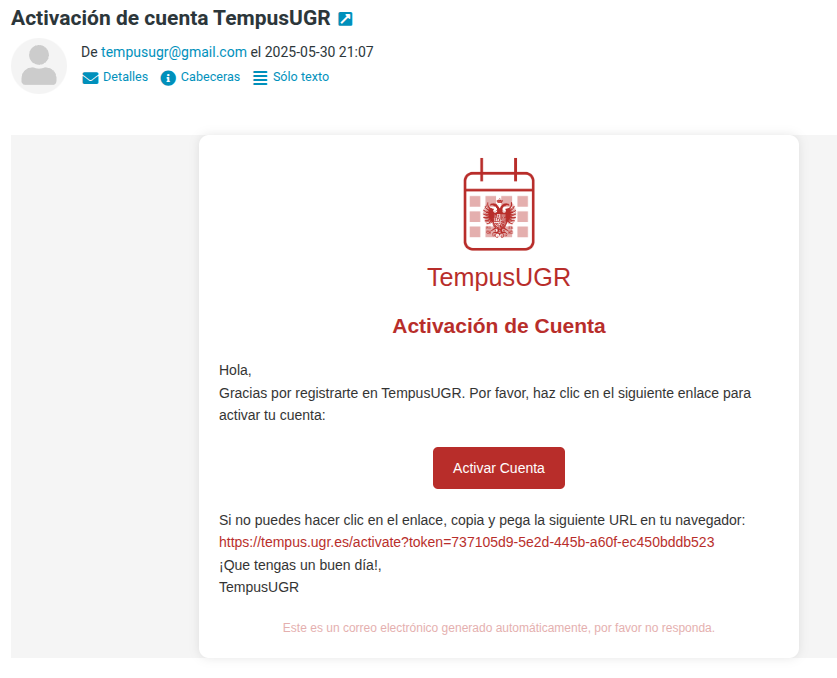
\includegraphics[width=0.8\textwidth]{figures/07_email.png}
    \caption{Correo de activación de cuenta}
    \label{fig:mail-service-class-diagram}
\end{figure}

\subsection{Auth Service}
El servicio de autenticación es el encargado de gestionar la autenticación de los usuarios del sistema. Este servicio se encarga de validar las credenciales de los usuarios y generar tokens JWT (JSON Web Tokens) para autenticar las solicitudes a otros servicios.
\newline\newline
Su lógica reside en la clase \texttt{AuthService}. 
La operación principal, \texttt{authenticate}, recibe las credenciales enviadas por el cliente y devuelve un par de tokens
\emph{JSON Web Token} (JWT): un \emph{access token} de corta duración y un \emph{refresh token} de duración más amplia. 

El proceso comienza verificando que la dirección de correo pertenezca a la Universidad de Granada; 
de lo contrario, se aborta la autenticación.  
Después, mediante un \texttt{WebClient} reactivo, el servicio consulta al microservicio de usuarios 
(\texttt{user-service}) para recuperar el \texttt{UserDTO} correspondiente.  
Si el usuario existe, está activo y la contraseña coincide con el \emph{hash} almacenado (comprobación
delegada a \texttt{PasswordUtil}), se generan ambos tokens.

\subsubsection*{Estructura del JWT}

Un JWT es una cadena en tres partes \emph{``header.payload.signature''}, codificadas en \texttt{Base64Url}.  
En este servicio se firma con el algoritmo simétrico \texttt{HS256}, usando la clave secreta
\lstinline|JWT_SECRET|:

\begin{verbatim}
Key key = Keys.hmacShaKeyFor(SECRET_KEY.getBytes(StandardCharsets.UTF_8));
String jwt = Jwts.builder()
        .setHeaderParam("typ", "JWT")
        .setSubject(id)              // Identificador del usuario
        .claim("role", role)         // Rol de la aplicación
        .setIssuedAt(new Date(now))
        .setExpiration(new Date(now + ttl))
        .signWith(key, SignatureAlgorithm.HS256)
        .compact();
\end{verbatim}

La cabecera (\texttt{header}) indica el tipo de token y el algoritmo de firma.  
El cuerpo (\texttt{payload}) almacena el identificador del usuario (\texttt{sub}), su rol y las marcas
temporal de emisión y caducidad (\texttt{iat}, \texttt{exp}).  
La firma garantiza la integridad: si cualquier byte del token cambia, la verificación falla.

\subsubsection*{Duración y refresco}

El \emph{access token} caduca en 24~horas (86,400,000~ms), su vida corta limita el riesgo ante robo.  
El \emph{refresh token} dura una semana y sólo sirve para
obtener nuevos \emph{access tokens}.  
La operación \texttt{refresh} valida la firma y la vigencia del \emph{refresh token};  
si supera la comprobación, crea un nuevo \emph{access token} manteniendo el \emph{refresh token} 
original mientras no haya expirado.  
El servidor no almacena sesiones, por lo que el mecanismo es \emph{stateless} y escalable: basta con
compartir la misma \lstinline|JWT_SECRET| entre las instancias.

\subsubsection*{Flujo de autenticación}

El diseño evita guardar estado en la base de datos y permite balancear las peticiones entre múltiples
réplicas sin afinidad de sesión.  

El flujo de autenticación y generación de tokens JWT se ilustra en la figura \ref{fig:auth-service-class-diagram}, donde se muestra cómo el servicio interactúa con el \texttt{user-service} para validar las credenciales y generar los tokens necesarios.

\begin{figure}[H]
    \centering
    \makebox[\textwidth][c]{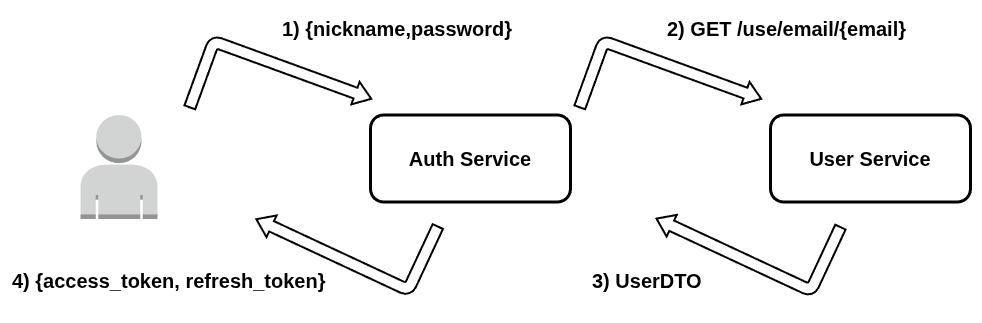
\includegraphics[width=1.1\textwidth]{figures/07_auth.png}}
    \caption{Flujo de autenticación y generación de tokens JWT}
    \label{fig:auth-service-class-diagram}
\end{figure}

\subsection{API Gateway}
El \texttt{api-gateway} actúa como el punto de entrada centralizado para todas las peticiones del sistema basado en microservicios. Está construido utilizando \textbf{Spring Cloud Gateway}, una solución reactiva que permite enrutar solicitudes a los distintos servicios internos, como \texttt{user-service} o \texttt{auth-service}. Su función no se limita al enrutamiento, sino que también gestiona aspectos transversales como la seguridad, la autenticación mediante JWT, y la validación de rutas públicas y protegidas.

\subsubsection{Spring Security en el Gateway}

\textbf{Spring Security} es un framework de seguridad potente y altamente configurable, que se utiliza para proteger tanto aplicaciones monolíticas como distribuidas. En el contexto del \texttt{api-gateway}, se emplea para interceptar las peticiones entrantes y aplicar mecanismos de autenticación antes de permitir el acceso a los servicios internos. Aquí no se gestionan sesiones, sino que se trabaja con tokens JWT (JSON Web Tokens), que son validados en cada petición.

El archivo \texttt{SecurityConfig} define la configuración de seguridad. En este componente se especifican:
\begin{itemize}
  \item Los filtros personalizados que deben ejecutarse antes del procesamiento de cada solicitud.
  \item Las rutas que deben ser públicas (por ejemplo, el login o el registro).
  \item Que el sistema funciona sin sesiones, usando una política \texttt{stateless}.
\end{itemize}

\subsubsection{Filtros personalizados}

Spring Security permite encadenar filtros que procesan las solicitudes antes de llegar a los controladores. En el gateway, se implementan dos filtros principales:

\paragraph{JwtAuthenticationFilter} Este filtro se encarga de interceptar todas las solicitudes entrantes y validar que el JWT (token de acceso) esté presente y sea válido. Para ello, extrae el token del encabezado \texttt{Authorization} y realiza una verificación utilizando una clave secreta compartida. En caso de éxito, el filtro añade los atributos del usuario autenticado al encabezado de la petición, de modo que los servicios internos puedan conocer la identidad y rol del usuario. Si el token no es válido o está ausente, la solicitud se rechaza con un error HTTP \texttt{401 Unauthorized}.

\paragraph{PathPrefixFilter} Elimina el prefijo /calendarugr/v1 de la ruta de cada petición entrante en el API Gateway. Si la URL comienza con ese prefijo, lo elimina y reescribe la ruta antes de pasar la petición al siguiente filtro o servicio interno. Así, los microservicios reciben rutas limpias y sin el prefijo de versión, facilitando el enrutamiento interno. Además, el filtro tiene la máxima prioridad para ejecutarse antes que otros filtros de seguridad.

\subsubsection{Configuración de rutas seguras}

En el archivo de configuración \texttt{SecurityConfig}, se define explícitamente qué rutas deben estar protegidas. Por ejemplo, aquellas que comienzan con \texttt{/user} pueden requerir un token JWT válido, mientras que rutas como \texttt{/auth/login} son públicas. Esta distinción permite implementar un control de acceso granular a través del propio gateway, centralizando así la lógica de seguridad.

Además, se utiliza una política de seguridad sin estado (\texttt{SecurityContextHolder.MODE\_INHERITABLETHREADLOCAL}) y se desactivan los mecanismos tradicionales como CSRF y sesiones HTTP, ya que todo el control de identidad se realiza mediante tokens.

En resumen, el \texttt{api-gateway} cumple un rol esencial en la arquitectura del sistema, actuando no solo como un proxy inverso, sino también como un punto de control de acceso. Gracias a Spring Security y a los filtros como \texttt{JwtAuthenticationFilter}, se logra una protección robusta y centralizada, adecuada para entornos distribuidos donde cada microservicio es independiente pero requiere información sobre la identidad del usuario que realiza la petición.

\subsection{RabbitMQ}
El servicio de mensajería RabbitMQ se integra en el sistema para facilitar la comunicación asíncrona entre los diferentes microservicios. Este enfoque permite desacoplar los servicios, mejorar la escalabilidad y manejar picos de carga sin afectar la disponibilidad del sistema.
\subsubsection{Configuración de RabbitMQ}
RabbitMQ se configura en el archivo \texttt{application.properties} de cada servicio que lo utiliza. Se especifican parámetros como el host del servidor RabbitMQ, el puerto, el nombre de usuario y la contraseña.
\subsubsection{Funcionamiento de RabbitMQ}

RabbitMQ es un sistema de mensajería basado en el modelo \textit{message broker}, que permite la comunicación asíncrona entre distintos servicios. Se apoya en el protocolo AMQP (\textit{Advanced Message Queuing Protocol}), un protocolo binario de capa de aplicación diseñado para asegurar la interoperabilidad entre sistemas, fiabilidad en la entrega de mensajes y soporte para confirmaciones, encolado y reintentos.

En una arquitectura de microservicios, RabbitMQ permite desacoplar componentes mediante el intercambio de mensajes a través de colas. Un servicio puede publicar un mensaje sin necesidad de que el receptor esté disponible en ese momento. Esta estrategia mejora la tolerancia a fallos y la escalabilidad del sistema.

\subsubsection{Componentes principales}

RabbitMQ se basa en cuatro componentes clave:

\begin{itemize}
  \item \textbf{Productores (Producers)}: servicios que envían mensajes. En este caso, el \texttt{user-service} actúa como productor.
  \item \textbf{Intercambios (Exchanges)}: puntos intermedios que reciben mensajes y los redirigen a una o más colas basándose en reglas de enrutamiento. Existen varios tipos, como \texttt{direct}, \texttt{fanout}, \texttt{topic} y \texttt{headers}.
  \item \textbf{Colas (Queues)}: estructuras donde los mensajes son almacenados hasta que un consumidor los procesa.
  \item \textbf{Consumidores (Consumers)}: servicios que reciben y procesan los mensajes. En este caso, el \texttt{mail-service} es el consumidor.
\end{itemize}

\subsubsection{Configuración en \texttt{user-service}}

El servicio \texttt{user-service} actúa únicamente como productor. Su configuración en \texttt{RabbitMQConfig} define un \texttt{DirectExchange} llamado \texttt{mail\_exchange}, y una clave de enrutamiento \texttt{registering\_routing\_key}. Esto implica que todos los mensajes enviados desde este servicio se publican a dicho \texttt{exchange} con esa clave.

\begin{verbatim}
DirectExchange exchange() {
    return new DirectExchange("mail_exchange");
}
\end{verbatim}

Este fragmento configura el punto de entrada de los mensajes que serán enviados al sistema de mensajería.

\subsubsection{Configuración en \texttt{mail-service}}

El servicio \texttt{mail-service} funciona exclusivamente como consumidor de mensajes, reflejada una configuración en la figura~\ref{fig:rabbitmq-config}. Su configuración es más extensa, ya que debe definir tanto las colas como las asociaciones con el intercambio, además de políticas de reintento y manejo de errores.

Se definen dos colas principales:
\begin{itemize}
  \item \texttt{registering\_queue}, para correos de confirmación de registro.
  \item \texttt{notification\_queue}, para notificaciones genéricas.
\end{itemize}

Ambas están enlazadas al \texttt{mail\_exchange} mediante sus respectivas claves de enrutamiento. Esta asociación se realiza mediante \texttt{Binding}.

También se especifica un convertidor de mensajes para que RabbitMQ utilice JSON como formato de serialización, mediante \texttt{Jackson2JsonMessageConverter}, permitiendo la compatibilidad con objetos Java.

\begin{figure}[H]
    \centering
    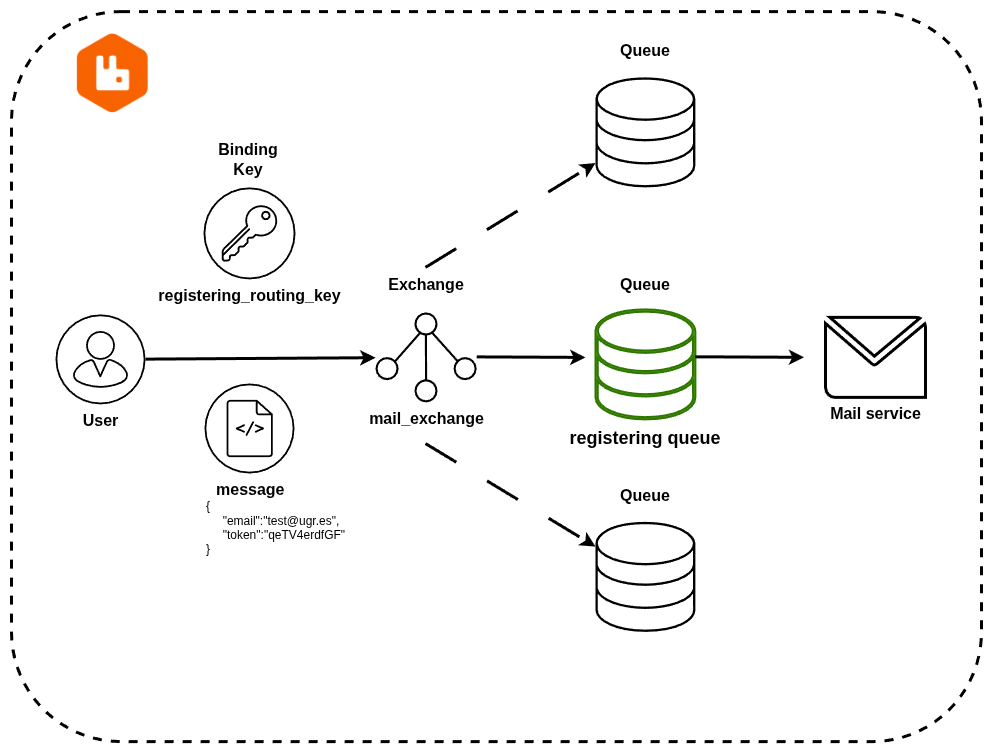
\includegraphics[width=0.8\textwidth]{figures/07_rabbit.png}
    \caption{Configuración de RabbitMQ en el servicio mail-service}
    \label{fig:rabbitmq-config}
\end{figure}

\subsubsection{Reintentos automáticos y Dead Letter Queues}

Una característica importante de la configuración es la gestión de reintentos automáticos y colas de mensajes muertos (DLQ).

Los reintentos se configuran a través de un \texttt{RetryInterceptor}:
\begin{verbatim}
.maxAttempts(3)
.backOffOptions(1000, 2.0, 50000)
\end{verbatim}
Esto indica que, si el procesamiento de un mensaje falla, se reintentará hasta tres veces, con un intervalo inicial de 1 segundo y un multiplicador exponencial. Si después de los reintentos no se logra procesar el mensaje, este se considera fallido.

En lugar de eliminar estos mensajes fallidos, se redirigen a una \textbf{Dead Letter Queue}, en este caso \texttt{mail\_dead\_letter\_queue}, asociada a su propio \texttt{Dead Letter Exchange} (\texttt{mail\_dead\_letter\_exchange}). Esto permite su análisis posterior, ya sea manual o mediante herramientas automáticas.

\subsubsection{Resumen funcional}

En este sistema, el \texttt{user-service} publica eventos de registro de usuarios a RabbitMQ. El \texttt{mail-service} escucha la cola correspondiente y envía los correos pertinentes. En caso de fallos temporales, se aplican políticas de reintento. Si el fallo persiste, el mensaje es redirigido a una DLQ, asegurando que ningún mensaje se pierde sin ser registrado.

Esta estrategia desacopla los servicios, mejora la resiliencia del sistema, y permite manejar errores de forma controlada sin interrumpir el flujo principal de la aplicación.

\subsection{Primer hito del backend}
El primer hito del backend se alcanza con la implementación de los servicios de autenticación y gestión de usuarios, junto con el servicio de correo electrónico. Estos servicios permiten registrar usuarios, autenticar sus credenciales y enviar correos electrónicos de confirmación. Además, se ha implementado el API Gateway para centralizar las peticiones y gestionar la seguridad mediante JWT.
\newline\newline
El siguiente paso antes de comenzar el siguiente sprint, y tras la reunión con Alberto Guillén Perales, es investigar cómo se pueden obtener los horarios de las asignaturas de la UGR.
\newline\newline
Para ello se investiga el sistema de scrapping, y se implementa un primer prototipo que permite obtener los horarios de las asignaturas de la UGR. Este prototipo se implementa en una primera aproximación del servicio \texttt{schedule-consumer-service}, que se encargará de consumir los horarios de las asignaturas y generar eventos a partir de ellos.
\newline
La tecnología seleccionada para realizar la tarea de scrapping es \textbf{Jsoup}, una biblioteca de Java que permite extraer y manipular datos de documentos HTML. Jsoup proporciona una API sencilla para navegar por el DOM, seleccionar elementos y extraer información, lo que facilita la tarea de scrapping.

\subsubsection{Scrapping con Jsoup}

El sistema realiza un proceso de extracción automatizado desde un portal académico para recopilar información sobre titulaciones, asignaturas, profesorado, grupos y horarios, utilizando técnicas de \textit{web scraping} con la biblioteca \texttt{Jsoup} y almacenamiento en base de datos mediante repositorios JPA.

La primera fase del proceso consiste en acceder al portal principal de ramas de conocimiento, desde donde se extraen los enlaces hacia las distintas titulaciones. A partir de cada enlace, se accede a la página específica de la titulación y se recogen sus datos básicos. Si la titulación no está ya registrada en la base de datos, se crea una nueva entrada con su nombre, URL y rama correspondiente.

Posteriormente, se recorre cada titulación almacenada y se accede a su página detallada para obtener dos tipos de información. Por un lado, si no se ha registrado la facultad correspondiente, se extrae de una tabla presente en el sitio web. Por otro lado, se recopilan los enlaces de todas las asignaturas que pertenecen a dicha titulación. Estas asignaturas se crean en la base de datos sólo si no existen previamente, y se asocian con la titulación correspondiente.

La última fase del proceso accede a cada una de las asignaturas almacenadas para extraer información detallada. En primer lugar, se recoge la información general de la asignatura como el curso académico, el año, el semestre, el tipo y el departamento responsable. Se aplican medidas de control como el recorte del texto del departamento si excede una longitud determinada.

Después, se identifica al profesorado vinculado a la asignatura y a sus respectivos grupos. Si el grupo ya existe, se actualiza su lista de profesores. Si no existe, se crea y se almacena junto con el nombre del profesor. Se contempla la posibilidad de que algunos grupos no aparezcan explícitamente en la web, en cuyo caso se generan automáticamente.

Finalmente, se extrae el horario de clases para cada grupo, identificando el día de la semana, aula, fechas de inicio y fin, y horas de inicio y fin. Esta información se transforma en objetos de clase que se asocian con el grupo correspondiente. Si no se detecta una clase idéntica en la base de datos, se crea una nueva entrada para ella.

El enfoque mostrado en la figura~\ref{fig:scrapping-process} permite consolidar una base de datos académica completa, dinámica y precisa, ideal para ser explotada por nuestro sistema.

%figura de scrapping, recortar un poco por arriba
\begin{figure}[H]
    \centering
    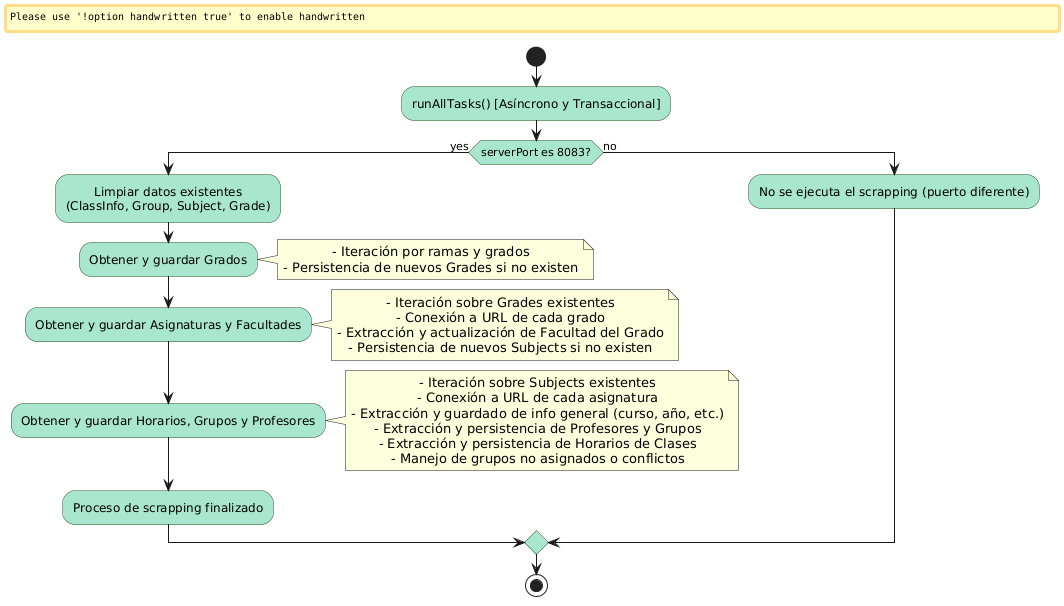
\includegraphics[width=1\textwidth, trim=0 0 0 45, clip]{figures/07_scrapping.png}
    \caption{Proceso de scrapping de asignaturas y horarios}
    \label{fig:scrapping-process}
\end{figure}

\section{Sprint 2}

En el comienzo de este sprint se continúa afinando y completando el script de scrapping, y revisando que se recoja información de todos los grados y asignaturas de la UGR. Esto se consigue realizando una labor de análisis exhaustivo de las diferentes páginas y secciones que conforman el portal de ``grados UGR'' mencionado con anterioridad.
\subsubsection{Schedule Consumer Service}
Paralelo a este desarrollo, se comienza el desarrollo del servicio \texttt{schedule-consumer-service}. Este es el encargado de, en primer lugar, hacer uso del scrapping para obtener los horarios de las asignaturas y almacenar la información en la base de datos, y en segundo lugar, de exponer endpoints relacionados con la consulta de estos datos. Uno de los objetivos de la realización se este servicio es poseer endpoints públicos para poder ser consumidos desde otros sistemas externos a nuestro frontend ``TempusUGR''.
\newline\newline
Una vez hecho el scrapping, y la información en base de datos (integrando el script de scrapping con el resto de componentes de Spring como lo son ``Repositories'',''Controllers'', etc), se necesita una manera de actualización de la información, puesto que es una de las premisas del sistema, mantener un acceso personalizado y actualizado del calendario académico.\newline
Para conseguir esto, y puesto que iterar y comprobar cambios sobre las más de 50.000 clases distintas impartidas en grupos de asignatura de la UGR es una tarea costosa y compleja, se decide implementar un ``\hypertarget{cronjob}{Cron job}'' que se encargue de realizar el scrapping de forma periódica, y así mantener la información actualizada. Este cron job se implementa en el servicio \texttt{schedule-consumer-service} y se ejecuta todos los días a las 00:00 horas, de forma que se actualizan los horarios de las asignaturas y se eliminan aquellos que ya no existen.
\newline\newline
Spring Boot proporciona una forma sencilla de implementar cron jobs mediante la anotación \texttt{@Scheduled}. Esta anotación permite definir un método que se ejecutará periódicamente según una expresión cron. En este caso, se ha configurado para que el método de actualización de horarios se ejecute diariamente a medianoche. Además de la anotación \texttt{@Scheduled}, se utiliza la anotación \texttt{@EnableScheduling} en la clase de configuración principal del servicio para habilitar el soporte de programación de tareas, y la anotación \texttt{@Async} para permitir la ejecución asíncrona de los métodos, lo que mejora la eficiencia y la capacidad de respuesta del servicio.
\newline
Para evitar un fallo del funcionamiento del servicio mientras se realiza una sustitución de los datos (Primero se borran los horarios antiguos, y luego se añaden los nuevos), se hace uso también de la anotación \texttt{@Transactional}, proveniente de ``Spring Transaction'', en el método que realiza la actualización de horarios. Esto asegura que todas las operaciones de base de datos se realicen dentro de una transacción, lo que garantiza la consistencia de los datos y evita problemas de concurrencia. Así los usuarios pueden seguir consultando la información de horarios sin  interrupciones, incluso durante el proceso de actualización.
\newline\newline
Una vez implementado el servicio se consigue el servicio troncal del backend, que permite obtener los horarios de las asignaturas de la UGR, y exponerlos a través de una API REST. Este servicio se convierte en el núcleo del sistema, ya que proporciona la información necesaria para el objetivo principal del proyecto: ofrecer un calendario académico personalizado y actualizado para los estudiantes de la UGR.

\subsubsection{Academic Subscription Service}
Así se comienza con el desarrollo del servicio \texttt{academic-subscription-service}, que se encargará de gestionar las suscripciones a los grupos de asignaturas de cualquier grado de la UGR.\newline
Las suscripciones se componen del identificador del usuario, la facultad, el grado, la asignatura y su grupo, puesto que de otra manera no se podría identificar de forma única un grupo de asignatura, ya que puede haber grupos con el mismo nombre en diferentes grados o facultades. Con esta información se hacen peticiones al servicio \texttt{schedule-consumer-service} para obtener los horarios de las asignaturas, flujo mostrado en la figura~\ref{classes}, y generar un calendario personalizado para el usuario con sus clases oficiales.\newline

\begin{figure}[H]
    \centering
    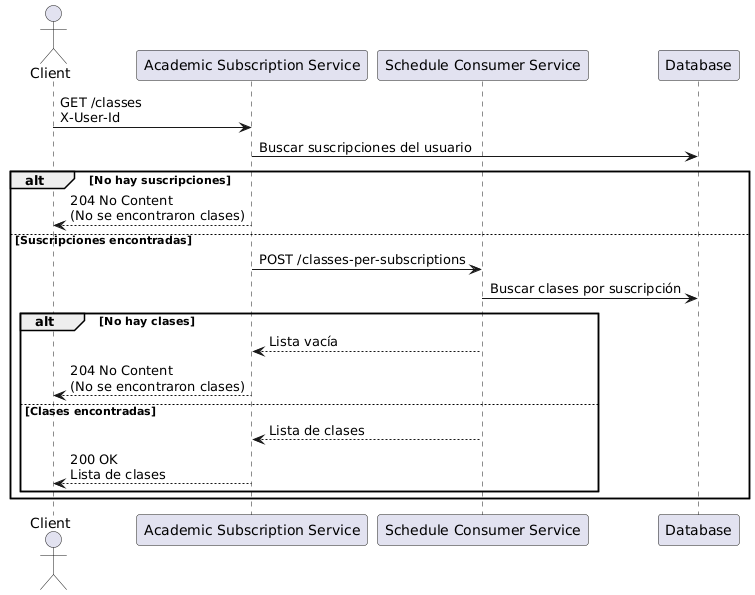
\includegraphics[width=0.95\textwidth]{figures/07_classes.png}
    \caption{Servicio de suscripciones académicas}
    \label{classes}
\end{figure}

Una vez se consigue esta información en formato ``JSON'', se implementa la lógica para generar un archivo \texttt{.ics}\cite{icalendar} que pueda ser importado en aplicaciones de calendario como Google Calendar, Outlook, etc. Para ello se utiliza la biblioteca \texttt{ical4j}, que permite crear y manipular archivos de calendario en formato iCalendar (\texttt{.ics}).\newline
\newline
Para crear esta primera versión de ``.ics'' se hace uso de los eventos recurrentes ( \texttt{RRULE}) de iCalendar, que permiten definir patrones de repetición para eventos. Esto es especialmente útil para las clases que se repiten semanalmente, ya que permite definir una sola entrada en el calendario que se repetirá automáticamente en las fechas correspondientes.\newline
\newline
Toda la información en este servicio se almacena en una base de datos no relacional, en este caso \texttt{MongoDB}, que permite una mayor flexibilidad y escalabilidad para almacenar los datos de las suscripciones y los horarios de las asignaturas. 

\subsubsection{Eureka Discovery Server}
A esta altura del proyecto en la que ya se tienen desarrollados varios servicios, se decide implementar un servidor de descubrimiento de servicios utilizando \textbf{Eureka}, que es parte del ecosistema de Spring Cloud. Eureka permite a los servicios registrarse y descubrir otros servicios en el sistema, facilitando la comunicación entre ellos sin necesidad de conocer sus direcciones IP o puertos específicos.
\newline 
Para conseguir esto se crea un nuevo proyecto de Spring Boot que actúa como el servidor Eureka. Este servidor se configura para permitir que otros servicios se registren y descubran entre sí. Cada servicio que se desea registrar en Eureka debe incluir la dependencia de \texttt{spring-cloud-starter-netflix-eureka-client} y configurarse adecuadamente en su archivo \texttt{application.properties}.
\newline
Esto nos permite los siguientes avances:
\begin{itemize}
  \item \textbf{Balanceo de carga}: Al registrar los servicios en Eureka, se pueden utilizar balanceadores de carga de manera dinámica, sin necesidad de configurar manualmente las direcciones IP y puertos de cada servicio. Eureka proporciona una lista de instancias disponibles, lo que permite al cliente elegir una instancia para enviar la solicitud.
  \item \textbf{Alta disponibilidad}: Si un servicio falla, Eureka permite que otros servicios sigan funcionando sin interrupciones, ya que pueden redirigir las peticiones a otras instancias disponibles.
  \item \textbf{Configuración centralizada}: Permite gestionar la configuración de los servicios desde un único punto, facilitando el mantenimiento y la actualización del sistema.
  \item \textbf{Facilidad de desarrollo}: Al utilizar Eureka, los desarrolladores pueden centrarse en la lógica de negocio de sus servicios sin preocuparse por la gestión de direcciones IP y puertos, ya que Eureka se encarga de ello. Es decir, las llamadas HTTP pasan de tener un formato similar a este \texttt{http://localhost:8081/calendarugr/v1/user-service/users} a \texttt{http://user-service/users}, donde \texttt{user-service} es el nombre del servicio registrado en Eureka.
\end{itemize}

De esta manera podemos tener un control de los servicios que se están ejecutando en el sistema, como se muestra en la figura~\ref{eureka}, y facilitar la comunicación entre ellos. Además, se puede escalar horizontalmente los servicios, añadiendo más instancias de un mismo servicio sin necesidad de modificar el código del cliente.

\begin{figure}[H]
    \centering
    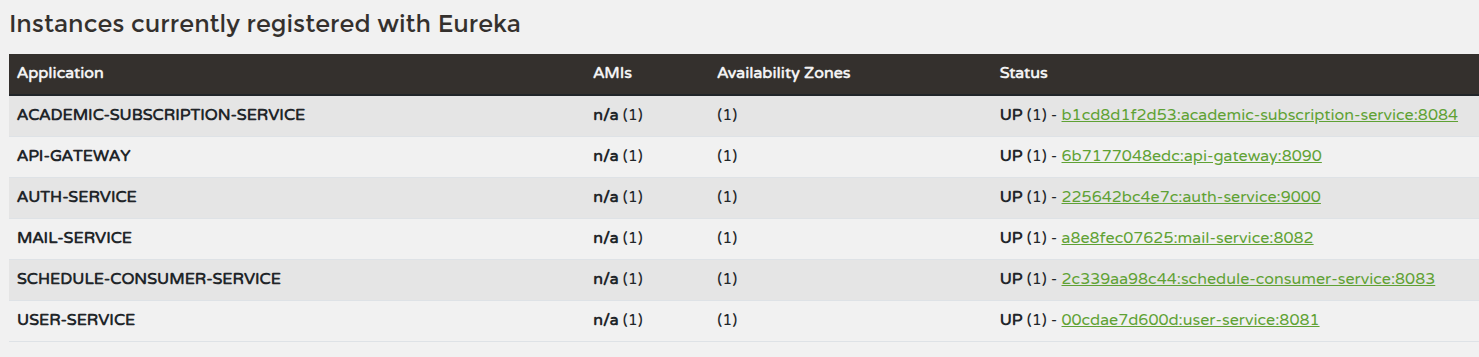
\includegraphics[width=1\textwidth]{figures/07_eureka.png}
    \caption{Servidor de descubrimiento de servicios con Eureka}
    \label{eureka}
\end{figure}

\section{Sprint 3}

El comienzo de estas tres semanas estuvo centrado en la finalización del servicio \texttt{academic-subscription-service}, que se encarga de gestionar las suscripciones a los grupos de asignaturas de cualquier grado de la UGR.\newline
Para conseguir esto, se implementa la gestión de eventos a nivel de grupo (eventos que son relevantes para aquellas personas suscritas a ese grupo de asignatura), y eventos a nivel de facultad (eventos que son relevantes para todas las personas suscritas a cualquier grupo de asignatura de esa facultad). Estos eventos se almacenan en la base de datos del servicio \texttt{academic-subscription-service}, en una tabla diferente a las suscripciones.\newline
Para poder crear estos eventos, el usuario debe ser tanto profesor como administrador, y para poder crear eventos a nivel de facultad, el usuario debe ser administrador. Estos eventos se crean a través de endpoints del servicio \texttt{academic-subscription-service}. 
\newline\newline
Una vez se crean los eventos, estos serán visibles para todos los usuarios suscritos a ese grupo de asignatura o facultad, y se enviarán notificaciones a través del servicio de correo electrónico (\texttt{mail-service}) a todos los usuarios suscritos con notificaciones activadas. Estas notificaciones se envían mediante RabbitMQ, como se ha explicado anteriormente, y se generan correos electrónicos personalizados utilizando plantillas Thymeleaf en el servicio de mail.
\newline\newline
Una vez creados los eventos, e implementada la posibilidad de poder obtener la información de estos y clases oficiales, se adaptó la creación de los archivos \texttt{.ics} para incluir tanto las clases oficiales como los eventos de grupo y facultad. Estos al contrario que las clases oficiales, no son recurrentes, por lo que se crean como eventos únicos en el calendario. De esta manera, el usuario puede importar un archivo \texttt{.ics} que contenga tanto sus clases oficiales como los eventos de grupo y facultad a su calendario personal, ya sea Google Calendar, Outlook, etc.\newline
\newline\newline
Además de esto se implementa la sincronización con Google Calendar. Para conseguir esto se pueden seguir diferentes estrategias:
\begin{itemize}
  \item \textbf{Google Calendar API}: Utilizar la API de Google Calendar para crear eventos directamente en el calendario del usuario. Esto requiere que el usuario autorice la aplicación a acceder a su calendario.
  \item \textbf{Exportación de archivos ICS}: Generar un archivo \texttt{.ics} que el usuario pueda descargar e importar manualmente en su Google Calendar.
  \item \textbf{Url de sincronización}: Proporcionar una URL de suscripción a un calendario que Google Calendar pueda utilizar para sincronizar automáticamente los eventos y clases oficiales.
\end{itemize}

En este caso, y como el sistema ya requiere el correo institucional al usuario (con el de google no podemos descifrar si es estudiante o docente), se opta por la tercera opción, que es la más sencilla y permite al usuario sincronizar su calendario de forma automática. Para ello se genera una URL que el usuario puede añadir a su Google Calendar, y que se actualizará automáticamente con los eventos y clases oficiales del usuario.
El acceso a esta URL es público, por lo que cualquier persona que tenga el enlace podrá acceder a los eventos y clases oficiales del usuario. Esto se decide hacer de esta manera para que Google Calendar pueda acceder a la información sin necesidad de autenticación, ya que el usuario ya ha autorizado la aplicación a acceder a su calendario al momento de crear la suscripción.
\newline
La fabricación de esta URL requiere la creación de un hash único para cada usuario que además sea ``reversible'' para identificar la pertenencia del mismo. Para conseguir esto se hizo uso de ``AES'', un algoritmo de cifrado simétrico que permite cifrar y descifrar datos de forma segura. Se utiliza una clave secreta para cifrar el identificador del usuario, y se genera un hash único que se utiliza como parte de la URL de sincronización. De esta manera, se garantiza que la URL es única para cada usuario y que solo el usuario puede acceder a su información.
\newline\newline
La URL queda con un formato similar a este: \texttt{https://tempus.ugr.es/calendarugr/v1/academic-subscription/calendar/{HASH}}

\subsubsection{Segundo hito del backend}

Con la implementación del servicio \texttt{academic-subscription-service} y la sincronización con Google Calendar, se alcanza el segundo hito del backend. Este hito permite a los usuarios suscribirse a grupos de asignaturas, recibir notificaciones de eventos relevantes y sincronizar su calendario personal con las clases oficiales y eventos de su facultad.

\subsubsection{Pruebas unitarias y de integración}
Se implementan pruebas unitarias para todos los servicios del backend, utilizando \textbf{JUnit} (librería de pruebas para Java) y \textbf{Mockito} (framework de simulación para pruebas unitarias). Estas pruebas permiten verificar el correcto funcionamiento de los servicios, asegurando que las funcionalidades implementadas cumplen con los requisitos establecidos. Se realizan pruebas tanto a nivel de unidad como de integración, comprobando que los servicios interactúan correctamente entre sí y con la base de datos.
\newline
Por ejemplo se implementan pruebas de integración en el servicio \texttt{schedule-consumer-service} para comprobar que todos los componentes del servicio funcionan correctamente, desde el scrapping de los horarios hasta la generación de los archivos \texttt{.ics}. Estas pruebas permiten detectar posibles errores en la lógica del servicio y asegurar que la información se almacena correctamente en la base de datos.
\newline
Algunos ejemplos de test en este servicio son:
\begin{itemize}
    \item \textbf{\texttt{testGetClassesFromGroup()}}:
    Este test verifica el \textit{endpoint} que devuelve las \textbf{clases de un grupo específico} (\texttt{/classes-from-group}). Simula una petición \texttt{GET} con parámetros para el grado, la asignatura y el grupo. Espera una respuesta exitosa (código \texttt{200 OK}) con contenido JSON que es un \textit{array}, y específicamente que el primer elemento tenga el día ``viernes''. También incluye un \texttt{System.out.println} para depuración de la \texttt{API Key} y la respuesta.

    \item \textbf{\texttt{testValidateExtraClass()}}:
    Este test prueba el \textit{endpoint} de \textbf{validación de clases extra} (\texttt{/extraclass-validation}). Envía una petición \texttt{POST} con un objeto \texttt{ExtraClassDTO} que contiene los detalles de una clase. Espera una respuesta exitosa (código \texttt{200 OK}) con contenido JSON que es una cadena \texttt{false}, lo que indica que la clase extra enviada no es válida según la lógica del \textit{backend}.

    \item \textbf{\texttt{testGetGrades()}}:
    Este test verifica el \textit{endpoint} que devuelve la \textbf{lista de grados} (\texttt{/grades}). Simula una petición \texttt{GET} y espera una respuesta exitosa (código \texttt{200 OK}) con contenido JSON que es un \textit{array}, y que ese \textit{array} contenga exactamente 6 elementos.

    \item \textbf{\texttt{testGetSubjectsGroups()}}:
    Este test prueba el \textit{endpoint} que devuelve las \textbf{asignaturas y sus grupos asociados} para un grado específico (\texttt{/subjects-groups}). Envía una petición \texttt{GET} con el parámetro \texttt{grade} y espera una respuesta exitosa (código \texttt{200 OK}) con un \textit{array} JSON. Verifica que el primer elemento del \textit{array} tenga la asignatura ``Cálculo'' y que su \textit{array} de grupos asociado contenga 22 elementos.

    \item \textbf{\texttt{testValidateSubscription()}}:
    Este test verifica el \textit{endpoint} de \textbf{validación de suscripciones} (\texttt{/subscription-validation}). Realiza dos pruebas \texttt{POST}:
    \begin{itemize}
        \item La primera envía una \texttt{SubscriptionDTO} \textbf{válida} y espera una respuesta \texttt{true}.
        \item La segunda envía una \texttt{SubscriptionDTO} \textbf{inválida} (con un grupo inexistente ``Z'') y espera una respuesta \texttt{false}. Ambas esperan un código \texttt{200 OK}.
    \end{itemize}

    \item \textbf{\texttt{testGetClassesFromGroup\_unauthorized()}}:
    Este test es una prueba de \textbf{seguridad o autorización}. Intenta acceder al mismo \textit{endpoint} \texttt{/classes-from-group} que el primer test, pero utiliza una \texttt{X-Api-Key} \textbf{incorrecta}. Espera que la respuesta sea un código \texttt{403 Forbidden}, indicando que la petición no está autorizada.
\end{itemize}

Ejemplos de test que comprueban la correcta interoperabilidad entre los servicios:

\begin{itemize}
    \item \textbf{\texttt{testConflictWithExistingClassMiddle()}}:
    Verifica que el \textit{backend} detecta un \textbf{conflicto de horario} cuando una clase extra propuesta se solapa con una clase existente en la base de datos (iniciando y terminando dentro del rango de la clase existente). Espera una respuesta de \texttt{status 409 Conflict}.

    \item \textbf{\texttt{testBadRequestNoFaculty()}}:
    Prueba la validación de entrada. Envía una petición para crear una clase extra donde el campo \texttt{facultyName} está \textbf{vacío}. Espera un \texttt{status 400 Bad Request}, indicando que el servidor ha rechazado la petición debido a datos inválidos o faltantes.

    \item \textbf{\texttt{testConflictWithExistingClassInit()}}:
    Comprueba que se detecta un \textbf{conflicto de horario} cuando la hora de inicio de la clase extra propuesta se solapa con una clase existente, aunque la hora de fin sea anterior al fin de la clase existente. Espera un \texttt{status 409 Conflict}.

    \item \textbf{\texttt{testConflictWithExistingClassFinish()}}:
    Asegura que se detecta un \textbf{conflicto de horario} cuando la hora de fin de la clase extra propuesta se solapa con una clase existente, aunque la hora de inicio sea posterior al inicio de la clase existente. Espera un \texttt{status 409 Conflict}.

    \item \textbf{\texttt{testConflictWithExistingClassFull()}}:
    Valida que se detecta un \textbf{conflicto de horario} cuando la clase extra propuesta abarca completamente el horario de una clase existente. Espera un \texttt{status 409 Conflict}.
\end{itemize}

En conjunto, estos test cubren la funcionalidad básica de varios \textit{endpoints} de la API (ejemplo de test pasados con éxito en la figura~\ref{test}), incluyendo la recuperación de datos, la validación de información y la comprobación de la seguridad por clave API.

\begin{figure}[H]
    \centering
    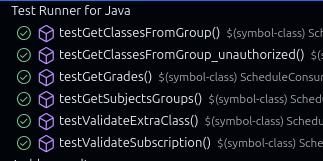
\includegraphics[width=0.55\textwidth]{figures/07_test.png}
    \caption{Pruebas unitarias e integración del servicio schedule-consumer-service}
    \label{test}
\end{figure}

\section{Sprint 4}

En este punto ya tenemos un backend sólido y funcional, con servicios que permiten gestionar usuarios, autenticación, suscripciones a asignaturas y horarios de la UGR. El siguiente paso es desarrollar el frontend de la aplicación, que permitirá a los usuarios interactuar con el sistema de manera intuitiva y visual.
\subsection{Frontend con Angular}
El frontend se desarrolla con Angular (versión 19.0.2), lo que significa que se utiliza TypeScript como lenguaje principal, junto con HTML y CSS para la estructura y el estilo de la aplicación. Angular es un framework de desarrollo web que permite crear aplicaciones de una sola página (SPA) de manera eficiente y escalable.
\subsubsection{Estructura del proyecto}
El proyecto de Angular se organiza en ``components'', ``services'' y ``models'', siguiendo las mejores prácticas de Angular. Los componentes son las unidades básicas de la interfaz de usuario, los servicios se encargan de la lógica de negocio y la comunicación con el backend, y los modelos definen las estructuras de datos utilizadas en la aplicación.
\subsubsection{Comunicación con el backend}
La comunicación con el backend se realiza a través de servicios que utilizan \texttt{HttpClient} de Angular para hacer peticiones HTTP a los diferentes \textit{endpoints} del API Gateway. Estos servicios manejan la autenticación mediante tokens JWT, que se envían en las cabeceras de las peticiones para identificar al usuario y su rol. Tanto el ``access\_token'' como el ``refresh\_token'' se almacenan en el almacenamiento local del navegador, lo que permite mantener la sesión del usuario activa entre recargas de página.

Además, también se ha hecho uso de ``Observables'' para manejar las respuestas del backend de manera asíncrona, lo que permite una experiencia de usuario más fluida y reactiva. Los servicios se encargan de transformar los datos recibidos del backend en objetos que pueden ser utilizados por los componentes de la interfaz de usuario.

Cada vez que se hace una petición al backend se hace uso de un ``Interceptor'' de Angular, este adjunta el token de acceso a la cabecera Authorization de casi todas las solicitudes salientes. Sin embargo, excluye ciertas rutas relacionadas con la autenticación inicial o el refresco de tokens (como /auth/login o /auth/refresh) para evitar bucles o requisitos innecesarios.
Si una solicitud protegida se realiza sin un token de acceso, el interceptor redirige al usuario a la página de login y lanza un error. Su función más importante es el manejo de tokens de acceso expirados: si una API devuelve un error 401, el interceptor intenta refrescar el token usando el token de refresco. Si el refresco es exitoso, actualiza el token de acceso y reintenta la solicitud original. Si el token de refresco también ha expirado, elimina ambos tokens, redirige al usuario al login y reporta un error. Para otros tipos de errores HTTP, simplemente los propaga.
\subsubsection{Rutas y navegación}
El enrutamiento se gestiona mediante el módulo de enrutamiento de Angular, que permite definir rutas para cada componente de la aplicación. Esto facilita la navegación entre diferentes vistas y componentes sin necesidad de recargar la página completa, lo que mejora la experiencia del usuario. Además, se implementa un sistema de guardias de ruta para proteger las rutas que requieren autenticación, asegurando que solo los usuarios con un token JWT válido puedan acceder a ellas.
\subsubsection{Interfaz de usuario}
La interfaz de usuario se ha desarrollado únicamente con HTML, CSS y Tailwind CSS, sin utilizar librerías de componentes adicionales. Esto permite un mayor control sobre el diseño y la apariencia de la aplicación, adaptándola a las necesidades específicas del proyecto. Se han creado componentes reutilizables para las diferentes secciones de la aplicación, como formularios de inicio de sesión, registro, suscripciones y visualización de horarios.
A continuación se muestran en las siguientes figuras (~\ref{login} , ~\ref{calendario} , ~\ref{sincro} , ~\ref{suscripciones} , ~\ref{eventos}) las páginas principales de la aplicación que incluyen el inicio de sesión, la página principal del calendario,la página de sincronización, la página de suscripciones y la página de eventos.

\begin{figure}[H]
    \centering
    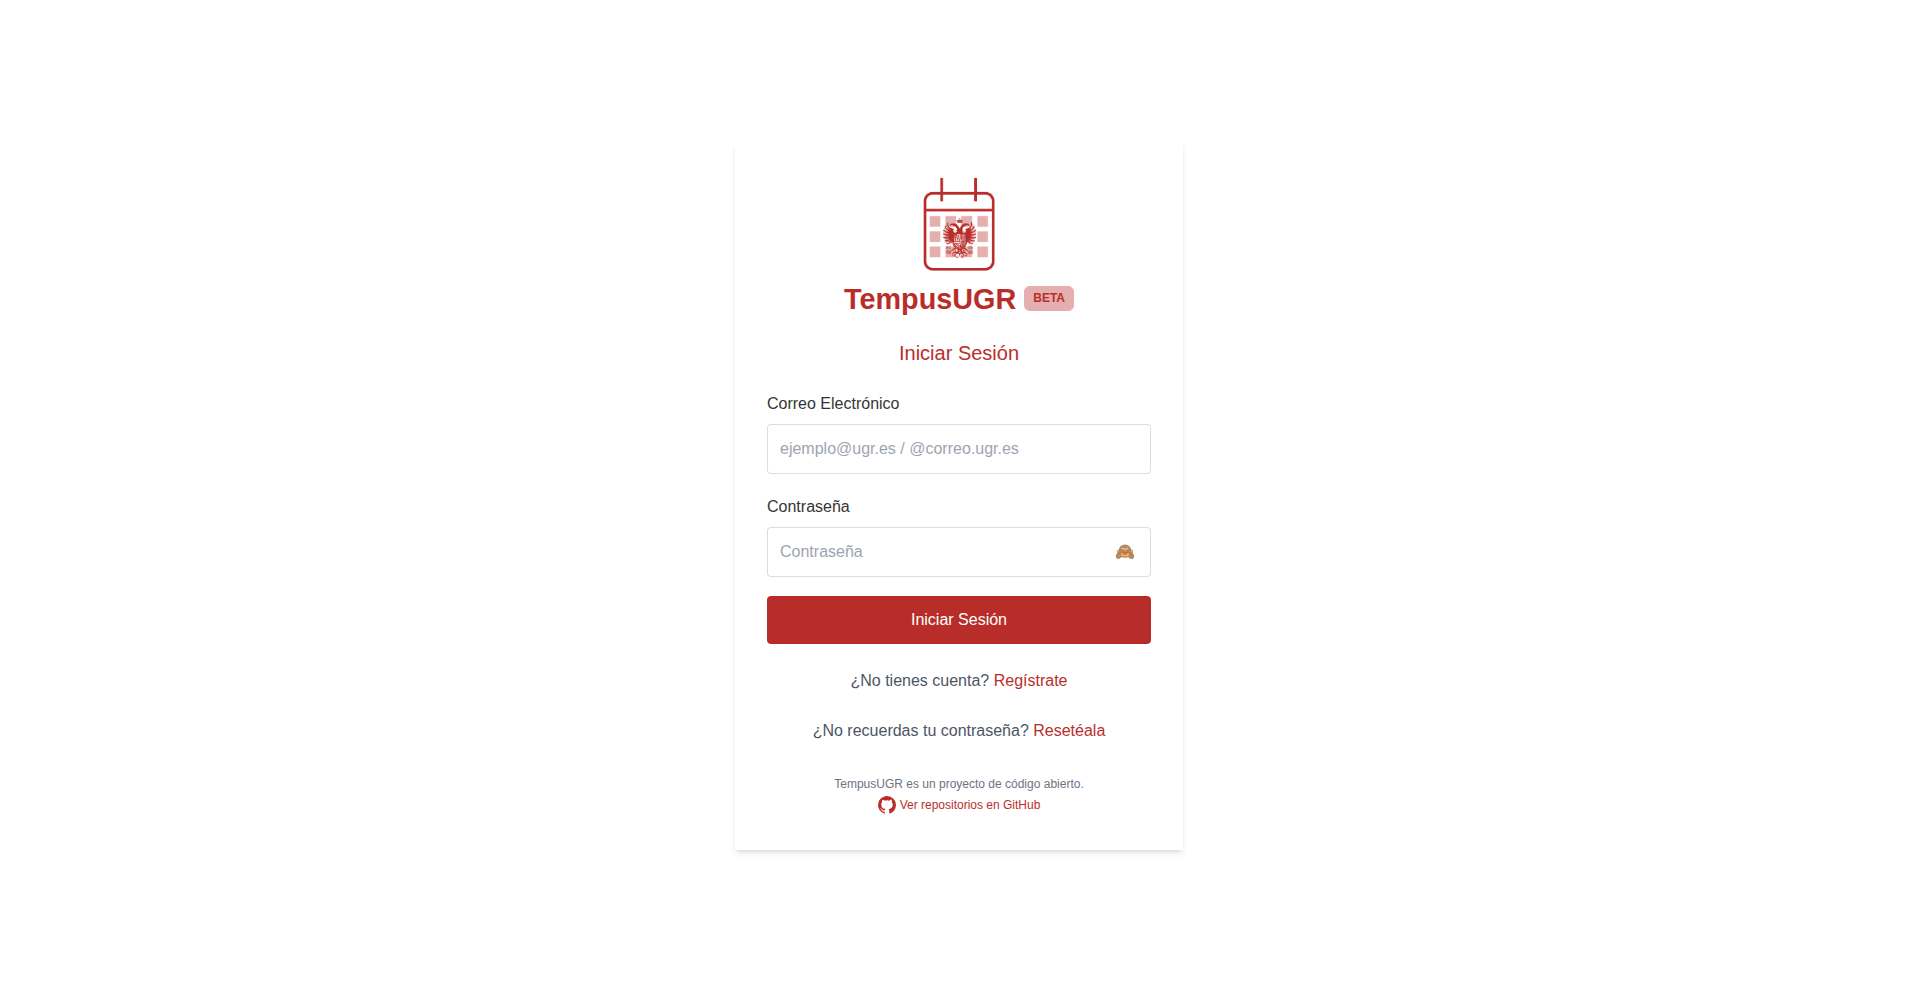
\includegraphics[width=1\textwidth]{figures/07_inicio.png}
    \caption{Página de inicio de sesión}
    \label{login}
\end{figure}
\begin{figure}[H]
    \centering
    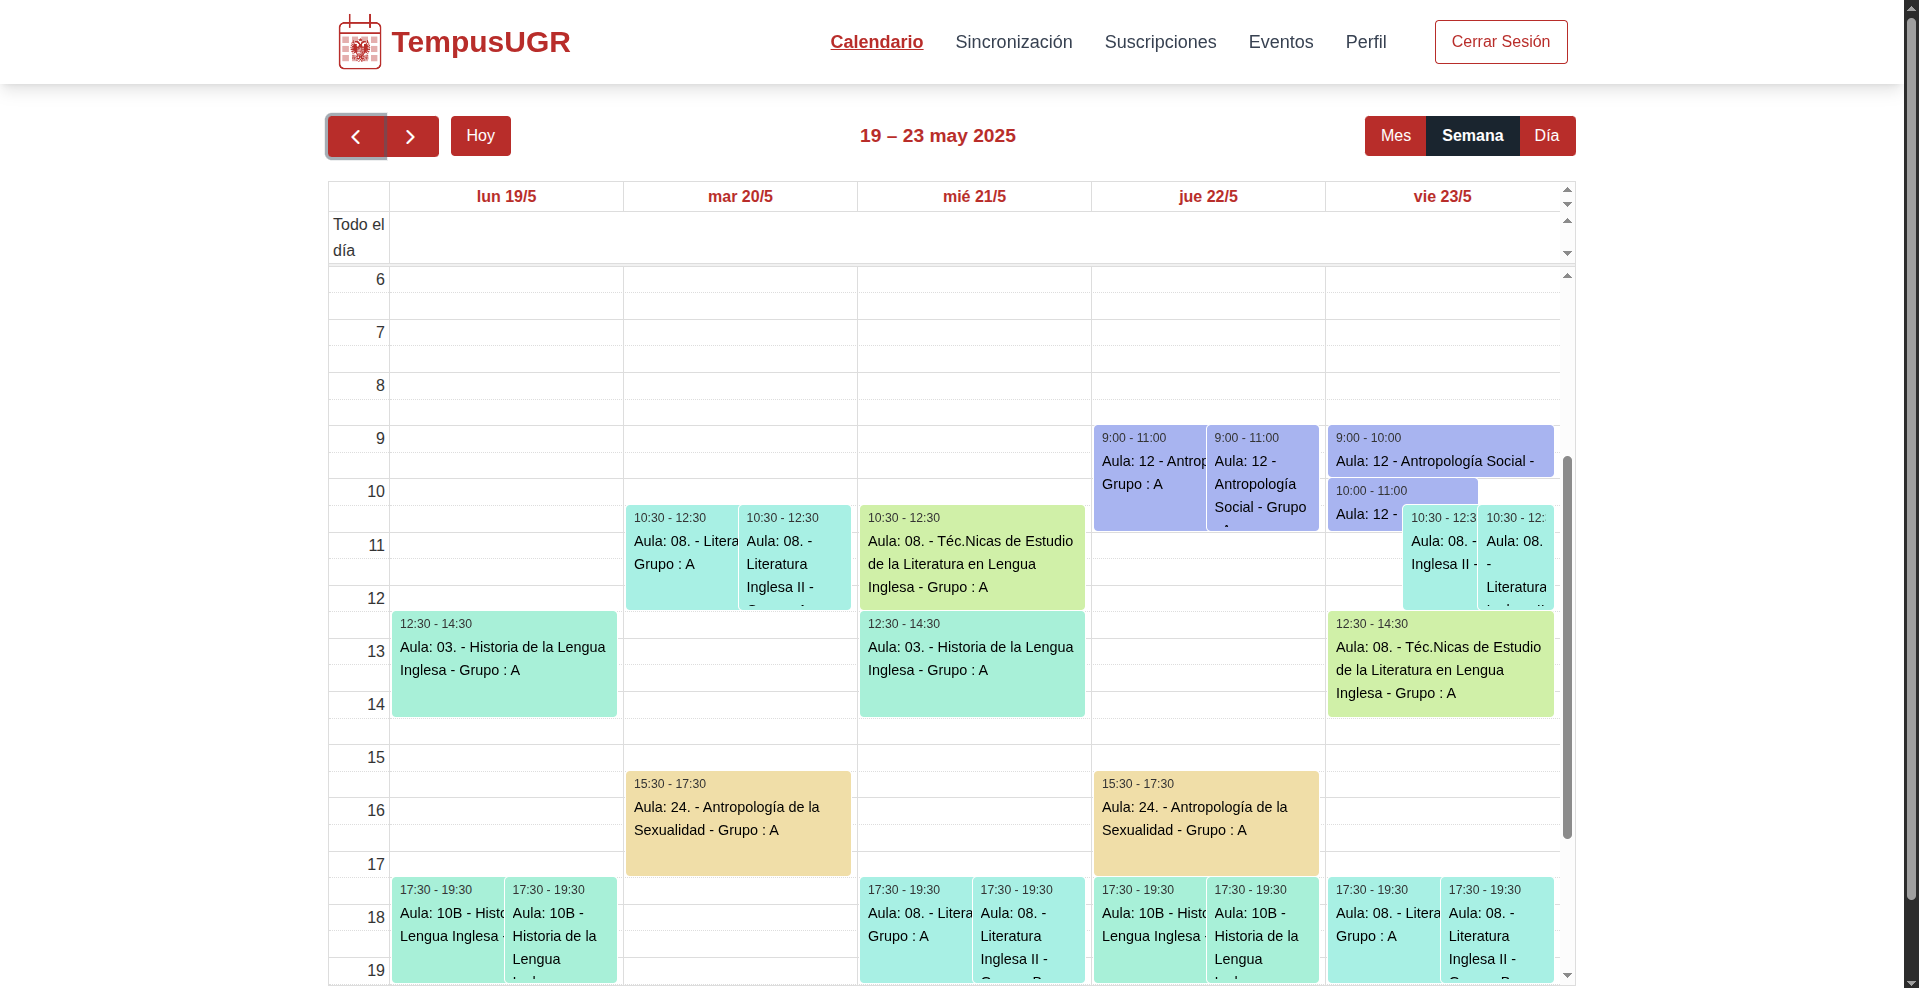
\includegraphics[width=1\textwidth]{figures/07_calendario.png}
    \caption{Página principal del calendario}
    \label{calendario}
\end{figure}
\begin{figure}[H]
    \centering
    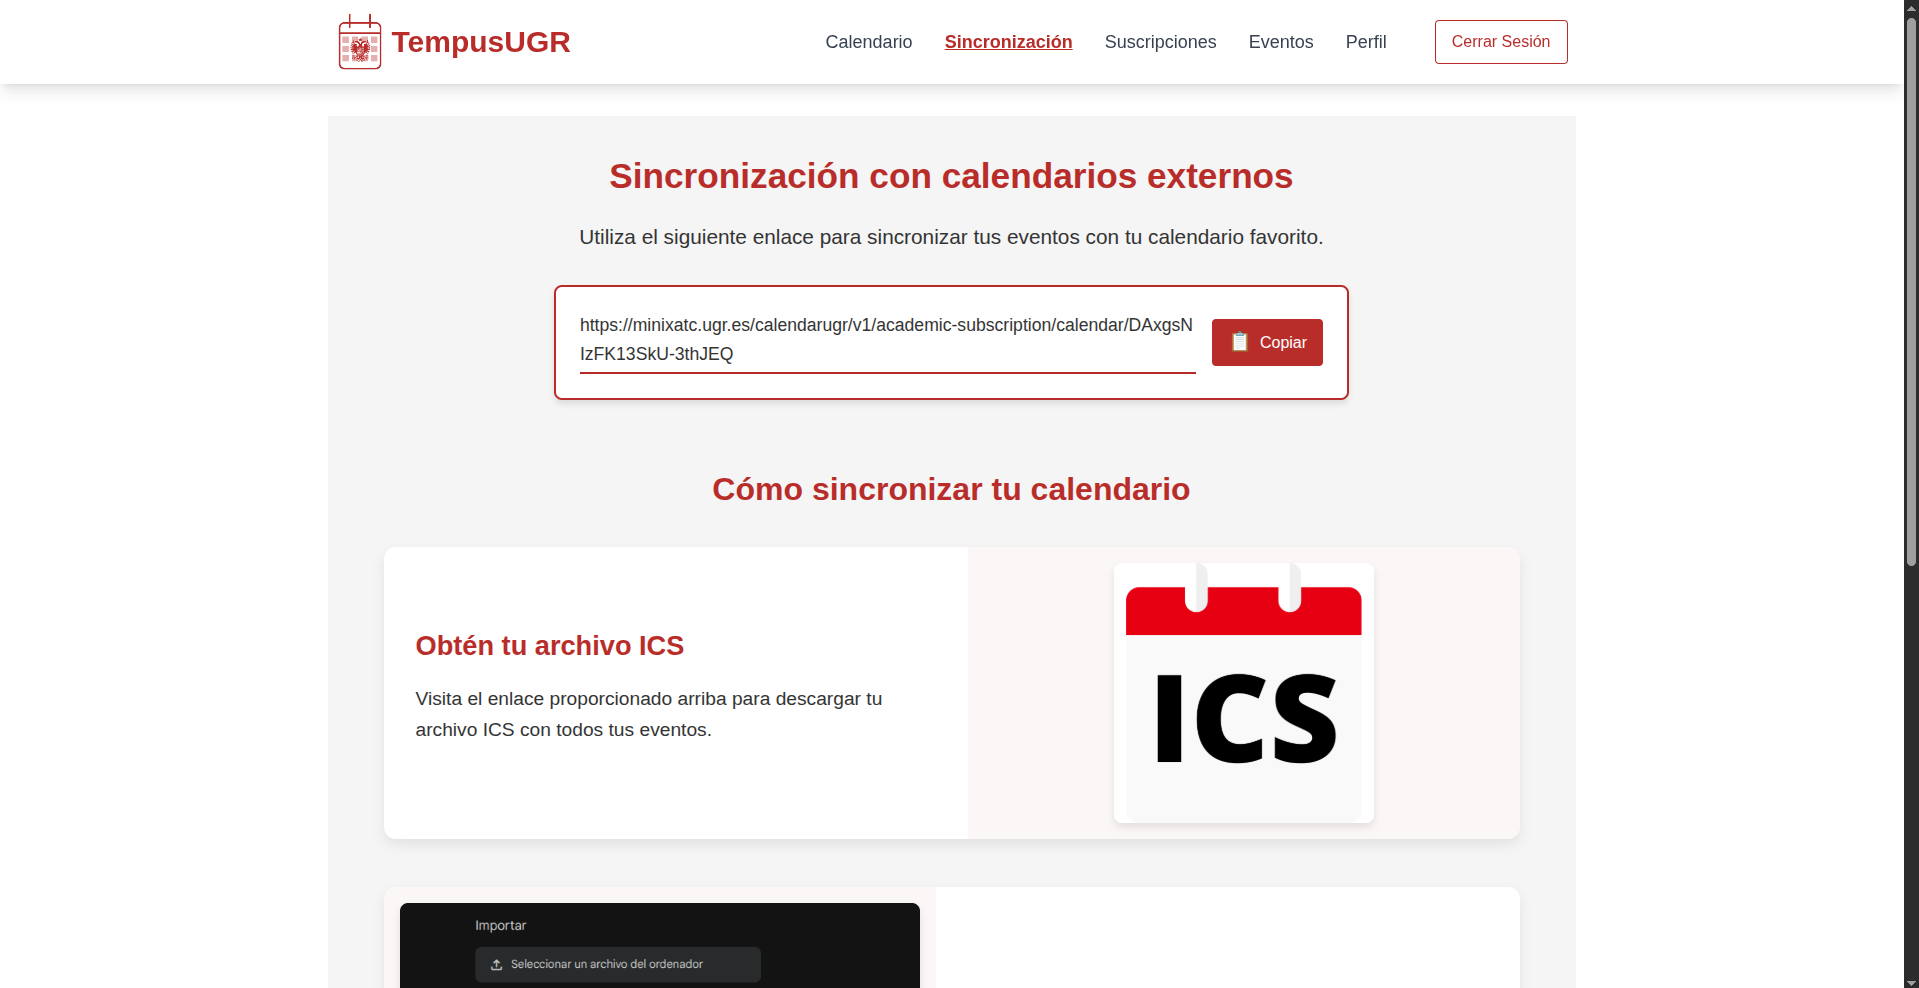
\includegraphics[width=1\textwidth]{figures/07_sincro.png}
    \caption{Página de sincronización con Google Calendar}
    \label{sincro}
\end{figure}
\begin{figure}[H]
    \centering
    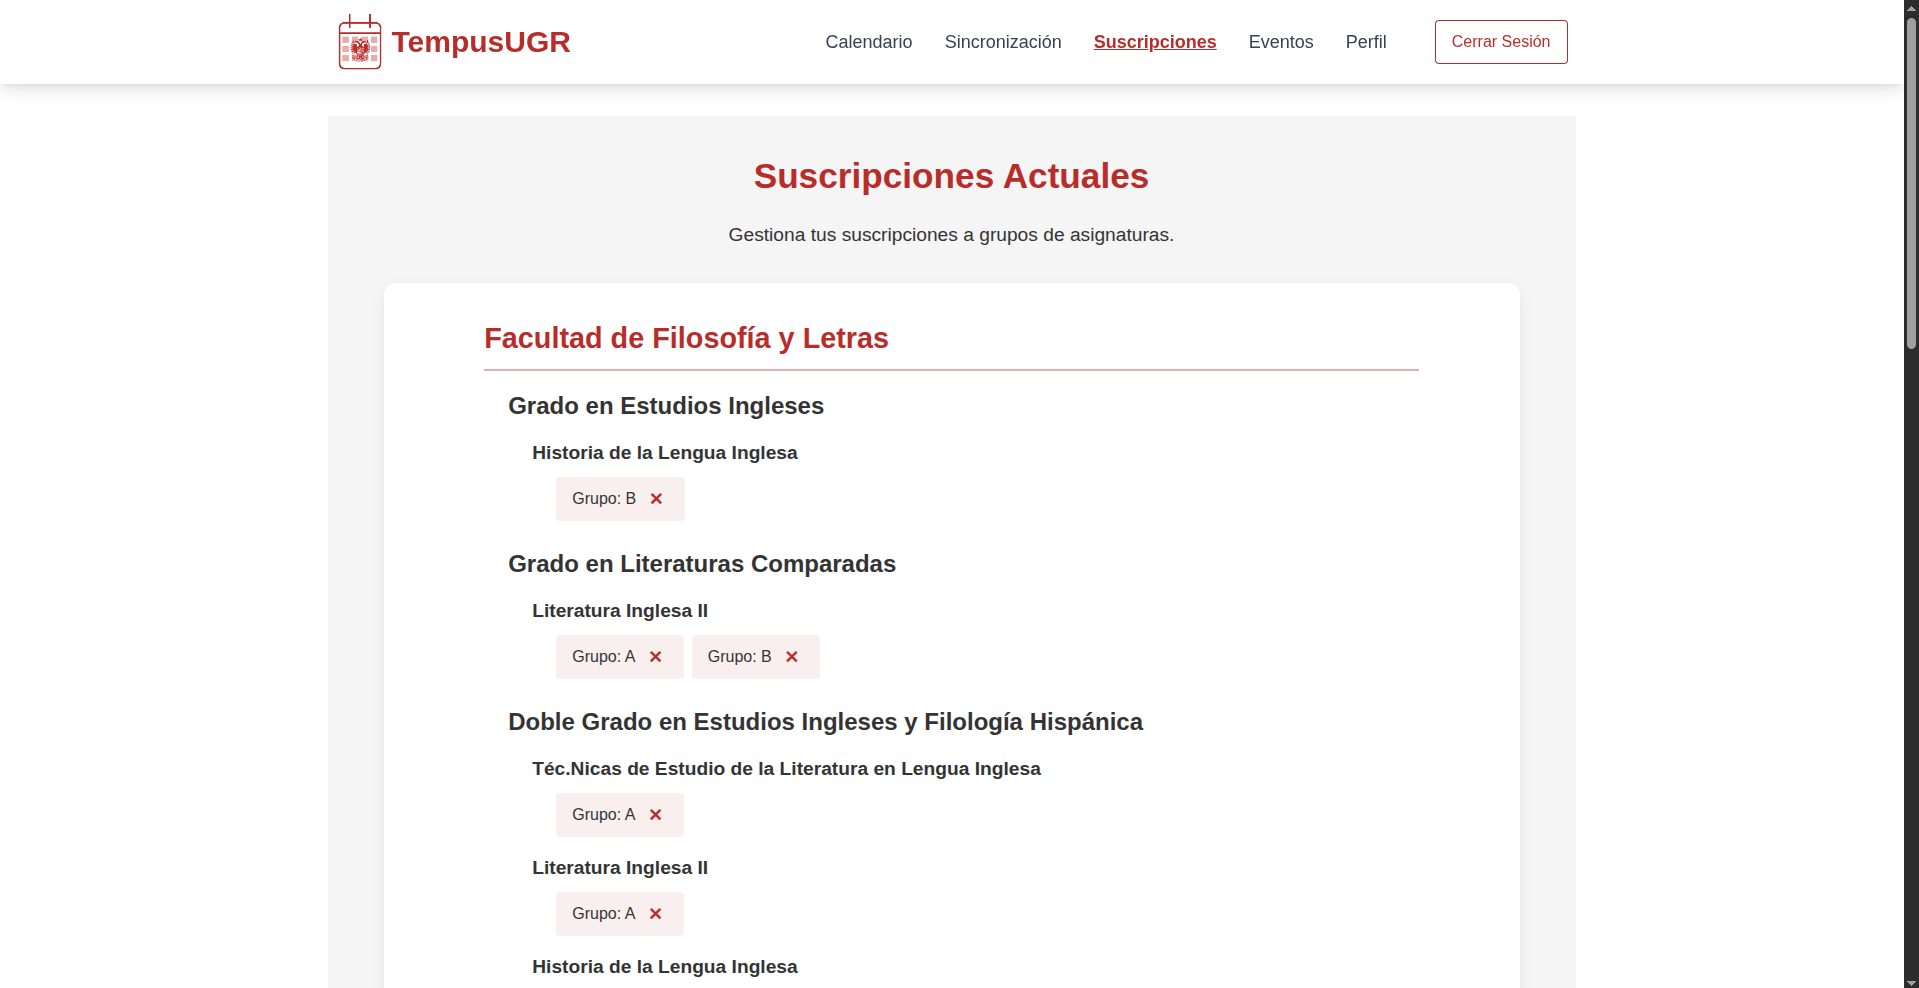
\includegraphics[width=1\textwidth]{figures/07_suscripciones.png}
    \caption{Página de suscripciones a asignaturas}
    \label{suscripciones}
\end{figure}
\begin{figure}[H]
    \centering
    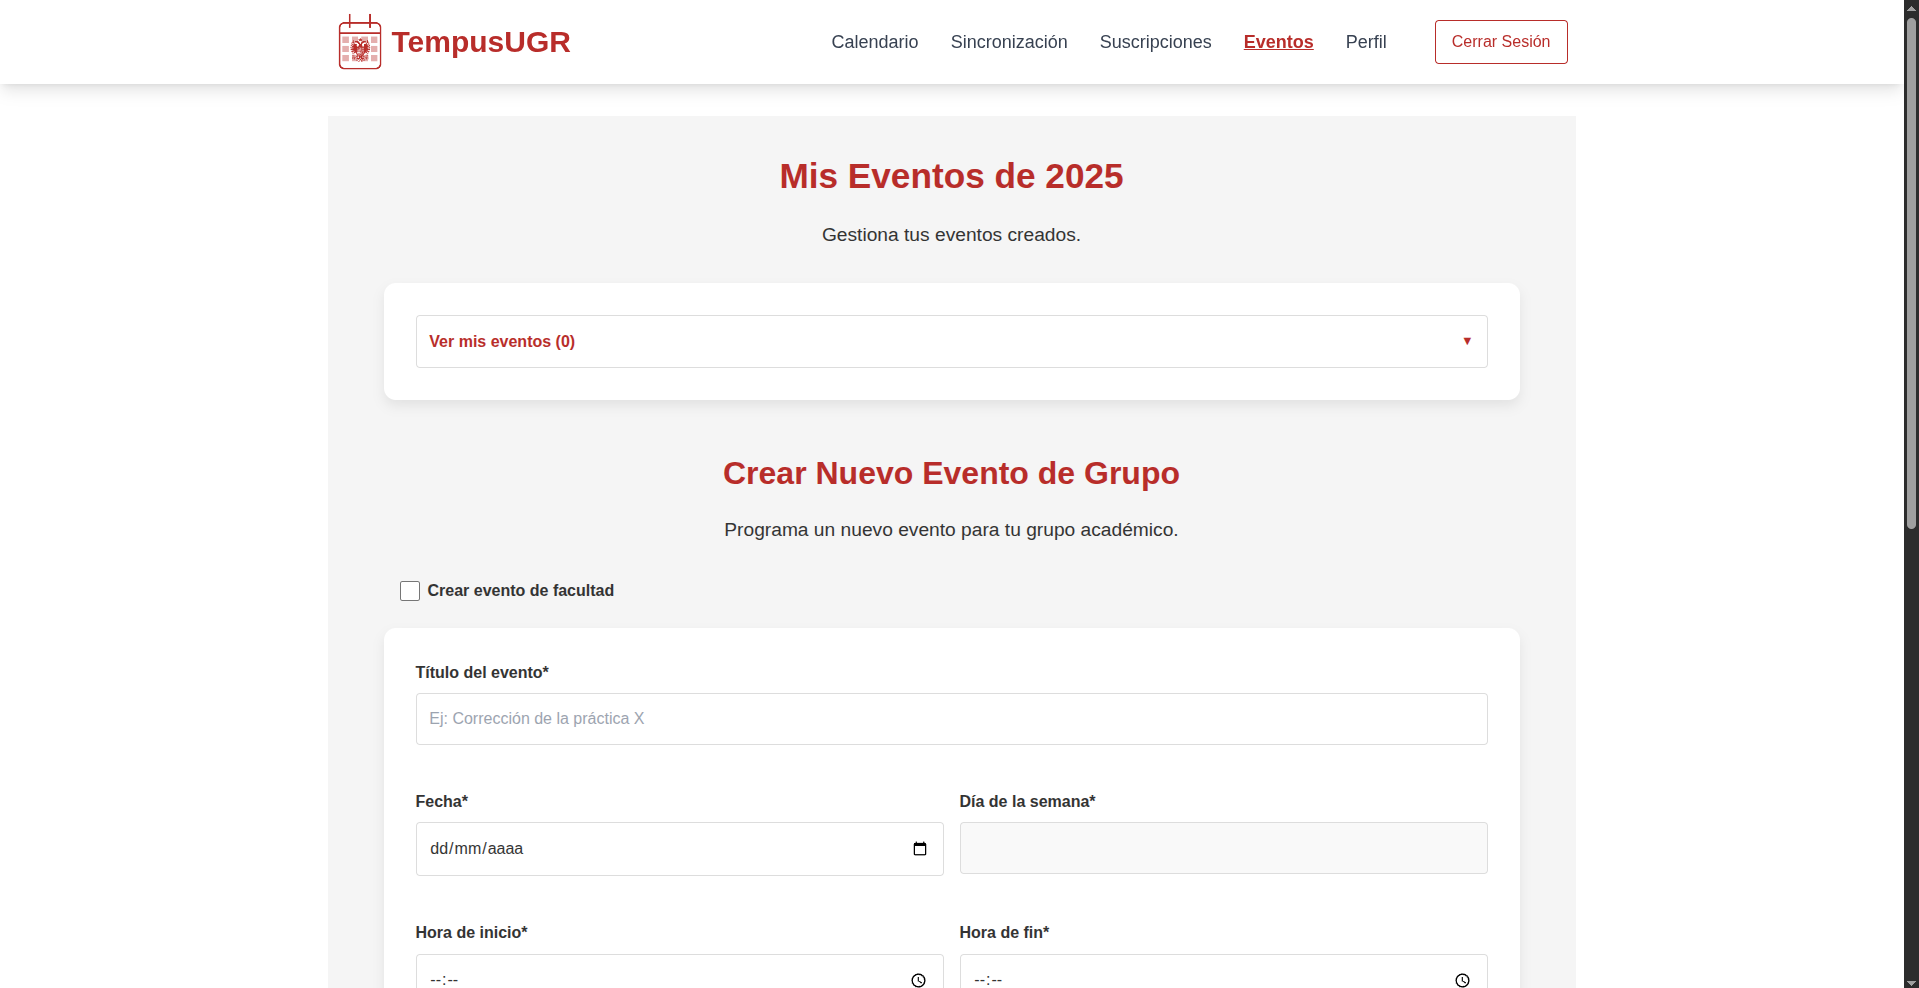
\includegraphics[width=1\textwidth]{figures/07_eventos.png}
    \caption{Página de eventos de grupo y facultad}
    \label{eventos}
\end{figure}

\subsubsection{Suscripción a las asignaturas de un profesor}
Al principio de este sprint se ajustaron tanto el ``Backlog'' como el ``Sprint Backlog'' para incluir la posibilidad de que un profesor pueda suscribirse a las asignaturas que imparte automáticamente buscando su nombre. Esta es una funcionalidad que se detectó como necesaria durante el desarrollo del frontend, ya que tenemos la información necesaria para poder implementarla, y es una funcionalidad que se espera que sea utilizada por los profesores de la UGR.
\newline
Al tener todos los servicios necesarios implementados, y funcionalidades similares ( obtener clases según grado, obtener todos los grados ...), no costó mucho tiempo y cambios significativos en el código. Se implementó un nuevo \textit{endpoint} en el servicio \texttt{schedule-consumer-service} que permite obtener las asignaturas de un profesor a partir de su nombre, y se añadió una nueva funcionalidad en el servicio \texttt{academic-subscription-service} que permite suscribirse a varias asignaturas a la vez.
Por otra parte en el apartado ``suscripciones'' se añadió un ``dropdown'' que sólo podrán visualizar los profesores y administradores, que les permitirá buscar por su nombre y suscribirse a todas sus asignaturas directamente.

\section{Sprint 5}

Las últimas tres semanas del desarrollo se destinaron a depurar y arreglar errores tanto en el frontend como en el backend. Además antes de comenzar este sprint también se hicieron modificaciones en el ``Backlog'' y el ``Sprint Backlog'' para añadir la funcionalidad de ``reseteo de contraseña''. Esta se detectó al hacer pruebas exhaustivas del sistema. Al pretender desplegar el sistema y que esté preparado para su uso, esta es una funcionalidad que se considera esencial para cualquier sistema de gestión de usuarios, y que no se había implementado hasta ahora.
\newline
Al contrario que en el sprint anterior, esta funcionalidad sí requiere de varios pasos para su implementación puesto que requiere, en el caso del backend, un endpoint para solicitar el reseteo, lógica para poder mandar un correo al usuario, y otro endpoint para modificar su contraseña, mientras que en el frontend se requerían un modal para solicitar un correo de contacto, y una página para establecer la nueva contraseña.

En todos los sprint, además de desarrollo, se ha destinado parte del tiempo para ir completando la documentación (diagramas, esquemas, redacción, etc), pero en este sprint se pretende completar la memoria.
\newline
Además al final, y tras este sprint, se despliega el sistema en un servidor de producción, y se realizan pruebas de carga y estrés para comprobar que el sistema es capaz de soportar un número elevado de usuarios concurrentes. Este apartado se desarrolla con más detalle en el apartado de ``Despliegue''\ref{cap:despliegue}.
    \chapter{Despliegue del sistema}\label{cap:despliegue}
Una vez desarrollado el sistema, es necesario desplegarlo en un servidor para que los usuarios de la UGR puedan hacer uso de él. Para ello, se ha optado por contenerizar el sistema utilizando Docker, lo que permite una fácil gestión y escalabilidad de los microservicios que componen la aplicación.
\newline\newline
\textbf{**Revisar este párrafo y detallar más si necesario}
El servidor en el que se despliega el sistema se encuentra en el edificio auxiliar de la ETSIIT. Fue solicitado por el director del TFG, Juan Luis Jiménez Laredo, y facilitado por el CSIRC (Servicio de Ciberseguridad y Respuesta a Incidentess Informáticos) de la UGR. El servidor cuenta con las siguientes características:

Además se solicitó una IP estática para el servidor, que se ha configurado para que apunte al dominio \texttt{tempus.ugr.es}. 
Esto se ha conseguido gracias a la colaboración del CSIRC, que ha configurado el DNS para que apunte al servidor y al dominio.

\section{Configuración del servidor}
Como paso previo a la contenerización del sistema y despliegue de la aplicación, se ha procedido a la configuración del servidor. 
\newline\newline
Esta configuración fue realizada tanto por el director como por el autor del TFG:
\begin{itemize}
    \item Creación de usuarios y grupos necesarios para el despliegue de la aplicación.
    \item Instalación de Docker y Docker Compose. Configuración de Docker para que se ejecute como servicio al iniciar el sistema.
    \item Configurar ssh para permitir el acceso remoto al servidor, y scp para la transferencia de archivos.
    \item Instalar git para poder clonar los repositorios necesarios.
\end{itemize}

No hubo más pasos previos a la contenerización del sistema, y en gran parte esta es la ventaja de contenerizar el sistema, ya que permite una fácil gestión y despliegue de la aplicación sin necesidad de realizar configuraciones complejas en el servidor.
\newline\newline
Sin hacer uso de esta tecnología se habrían tenido que realizar, entre otros, los siguientes pasos:
\begin{itemize}
    \item Configuración de un servidor web (Apache) para servir la aplicación.
    \item Configuración de un servidor de base de datos (MySQL y MongoDB) para almacenar los datos de la aplicación.
    \item Instalación y configuración de Java y Maven para compilar y ejecutar los microservicios.
    \item Instalación y configuración de Node.js y Angular CLI para compilar el frontend de la aplicación.
    \item Configuración de un servidor de mensajería (RabbitMQ) para la comunicación entre microservicios.
    \item etc
\end{itemize}

Para acceder al servidor de manera remota se ha utilizado la VPN de la UGR, que permite conectarse al servidor de forma segura y acceder a los recursos de la red de la universidad.
\newline
Y para el paso de archivos entre el servidor y el equipo local se ha utilizado el protocolo SCP (Secure Copy Protocol), que permite transferir archivos de forma segura a través de SSH.
\section{Contenerización del sistema}

El primer paso realizado en este sentido ha sido la contenerización del backend del sistema, que está compuesto por varios microservicios. 

\subsection{Pasos para la contenerización del backend}

En esta primera fase se han contenerizado, construido y levantado los servicios de la siguiente manera:

\begin{enumerate}
    \item Crear una red en docker:
    \begin{lstlisting}[language=bash]
        docker network create calendarugr
    \end{lstlisting}
    \item Generar los .jar de los microservicios, sin pasar los tests para una construcción sin conflictos para los servicios que ya están contenerizados:
    \begin{lstlisting}[language=bash]
        ./mvnw clean package -DskipTests
    \end{lstlisting}
    \item Crear las imágenes de los microservicios (Ej imagen de Eureka service):
    \begin{lstlisting}[language=bash]
        FROM amazoncorretto:21-alpine-jdk
        WORKDIR /app
        EXPOSE 8761
        COPY ./target/eureka-service-0.0.1-SNAPSHOT.jar eureka-service.jar

        ENTRYPOINT ["java", "-jar", "eureka-service.jar"]
    \end{lstlisting}
    \item Construir la imagen de docker:
    \begin{lstlisting}[language=bash]
        docker build -t eureka-service .
    \end{lstlisting}
    \item Para levantar los contenedores uno a uno (Ej levantando el contenedor de Eureka):
    \begin{lstlisting}[language=bash]
        docker run -d --name eureka-service --network calendarugr -p 8761:8761 eureka-service
    \end{lstlisting}
    \item Bajar las imágenes oficiales de mysql:8.0.41 y mongo:6.0.4, además de las imágenes de RabbitMQ:
    \begin{lstlisting}[language=bash]
        docker pull mysql:8.0.41
        docker pull mongo:6.0.4
        docker pull rabbitmq:3-management
    \end{lstlisting}
    \item Para levantar contenedores con variables de entorno (Ej levantando el contenedor de Mysql):
    \item \begin{lstlisting}[language=bash]
        docker run -p 3307:3306 --network calendarugr \
            -e MYSQL_ROOT_PASSWORD=...\
            -e MYSQL_USER=... \
            -e MYSQL_PASSWORD=... \
            -v /home/juanmi/mysql-scripts/init.sql:/docker-entrypoint-initdb.d/init.sql \
            --name mysql \
            mysql:8.0.41
    \end{lstlisting}
    \item El init.sql es un script que se ejecuta al iniciar el contenedor de Mysql, y se utiliza para crear la base de datos y las tablas necesarias para el funcionamiento del sistema. El script se encuentra en la carpeta \texttt{mysql-scripts} del proyecto.
    \begin{lstlisting}[language=sql]
        CREATE DATABASE IF NOT EXISTS DB_USER_SERVICE;
        CREATE DATABASE IF NOT EXISTS DB_SCHEDULE_CONSUMER_SERVICE;

        GRANT ALL PRIVILEGES ON DB_USER_SERVICE.* TO 'calendarugr'@'%';
        GRANT ALL PRIVILEGES ON DB_SCHEDULE_CONSUMER_SERVICE.* TO 'calendarugr'@'%';
        FLUSH PRIVILEGES;
    \end{lstlisting}
    \item Para levantar el contenedor de Mongo:
    \begin{lstlisting}[language=bash]
        docker run -d --name mongodb \
            -p 27018:27017 \
            --network calendarugr \
            -e MONGO_INITDB_ROOT_USERNAME=... \
            -e MONGO_INITDB_ROOT_PASSWORD=... \
            mongo:6.0.4
    \end{lstlisting}
\end{enumerate}

De esta manera se levantan todos los servicios uno a uno y se pueden probar de forma individual y en conjunto. Sin embargo, para facilitar el despliegue y la gestión de los microservicios, se ha optado por utilizar Docker Compose.

\subsection{Docker Compose}
Docker Compose es una herramienta que permite definir y ejecutar aplicaciones Docker multi-contenedor. Con Docker Compose, se puede definir la configuración de todos los microservicios en un único archivo \texttt{docker-compose.yml}, lo que facilita su gestión y despliegue.
\newline\newline
Este enfoque nos permite centralizar la configuración de todos los microservicios en un único archivo, lo que facilita su gestión y despliegue, de manera que:
\begin{itemize}
    \item Cada microservicio se define como un servicio en el archivo \texttt{docker-compose.yml}.
    \item Se especifican las imágenes de cada microservicio, los puertos que se exponen, las redes a las que pertenecen y las variables de entorno necesarias.
    \item Se definen las dependencias entre los servicios, lo que permite que Docker Compose gestione el orden de inicio de los contenedores.
    \item Se pueden definir volúmenes para persistir los datos de los servicios, como en el caso de MySQL y MongoDB.
\end{itemize}

De esta manera lo único que haría falta en el servidor para levantar todo el backend sería un directorio contenedor del archivo \texttt{docker-compose.yml}. Al tener este archivo referencia a las imágenes oficiales de MySql, Mongo y RabbitMQ, además de las imágenes de los servicios subidos a Docker Hub, no es necesario tener las imágenes construidas en el servidor, ya que Docker Compose se encargará de descargarlas automáticamente al levantar los servicios.

Para levantar todos los servicios definidos en el archivo \texttt{docker-compose.yml}, se puede ejecutar el siguiente comando:
\begin{lstlisting}[language=bash]
    docker-compose up -d ( -d para que se levanten en segundo plano)
\end{lstlisting}

Además para facilitar aún se han creado automatizaciones para la construcción de las imágenes y el despliegue de los microservicios, de manera que se pueden ejecutar los siguientes comandos:
\begin{lstlisting}[language=bash]
    ./build_services.sh 
    ./upload_to_hub.sh
\end{lstlisting}

Estos scripts se encargan de construir las imágenes de los microservicios y subirlas al repositorio de Docker Hub, lo que permite que se puedan desplegar en cualquier servidor con Docker instalado.

\subsection{Pasos para la contenerización del frontend}

El frontend del sistema está desarrollado en Angular y se ha decidido contenerizarlo utilizando Apache como servidor web. A continuación se detallan los pasos realizados para la dockerización del frontend:

\begin{enumerate}
    \item Construir el proyecto Angular para producción:
    \begin{lstlisting}[language=bash]
        ng build --configuration production
    \end{lstlisting}
    Este comando generará una carpeta \texttt{dist} con los archivos necesarios para desplegar la aplicación. Estos serán trasladados a un directorio del servidor, por ejemplo, \texttt{built\_tempus}, y deberá estar disponible en el mismo directorio que el docker-compose.yml, los certificados, y un directorio ``apache'' con el archivo de configuración de Apache y el Dockerfile.
    \newline
    Además, dentro del directorio \texttt{built\_tempus} se debe crear un archivo \texttt{.htaccess} con el objetivo de redirigir todas las peticiones al archivo \texttt{index.html} del frontend, para que Angular pueda manejar el enrutamiento de la aplicación. El contenido del archivo \texttt{.htaccess} es el siguiente:
    \begin{lstlisting}[language=bash]
        RewriteEngine On
        RewriteBase /
        RewriteRule ^index\.html$ - [L]
        RewriteCond %{REQUEST_FILENAME} !-f
        RewriteCond %{REQUEST_FILENAME} !-d
        RewriteRule . /index.html [L]
    \end{lstlisting}
    \item Solicitar los certificados SSL necesarios para el dominio \texttt{tempus.ugr.es}. Estos certificados son necesarios para habilitar HTTPS en el servidor web, y habilitarlo tanto para el frontend como para el backend.
    \item Copiar los certificados SSL en una carpeta del servidor, por ejemplo, en \texttt{/home/user/certificates}. Estos certificados son necesarios para habilitar HTTPS en el servidor web.
    \item Crear un archivo de configuración para Apache (\texttt{apache-ssl.conf}) en el que se especifique la configuración del servidor web.
          Aquí se especifican el uso de SSL, la redirección de HTTP a HTTPS y la configuración del \hyperlink{reverseproxy}{Reverse Proxy} para el backend.
        \begin{lstlisting}[language=bash] 
            <VirtualHost *:443>
                ServerName tempus.ugr.es
                ServerAlias xxx.xx.xxx.xxx

                # Directorio raiz donde se encuentra tu aplicacion Angular
                DocumentRoot /var/www/html

                # Habilitar SSL
                SSLEngine on
                SSLCertificateFile /ejemplo/de/ruta/certificado.pem                
                SSLCertificateKeyFile /ejemplo/de/ruta/clave-privada.pem

                # Configuracion de cifrados seguros
                SSLCipherSuite "HIGH:MEDIUM:!MD5:!RC4:!3DES"
                SSLHonorCipherOrder on

                # Protocolos seguros
                SSLProtocol -all +TLSv1.2 +TLSv1.3

                SSLProxyEngine On
                SSLProxyProtocol -all +TLSv1.2
                SSLProxyCheckPeerCN off
                SSLProxyCheckPeerName off

                # PROXY PARA EL API GATEWAY
                ProxyPass /calendarugr/v1 http://api-gateway:8090/calendarugr/v1
                ProxyPassReverse /calendarugr/v1 http://api-gateway:8090/calendarugr/v1

                <Directory /var/www/html>
                        Options Indexes FollowSymLinks
                        AllowOverride All
                        Require all granted
                    </Directory>

                    ErrorLog ${APACHE_LOG_DIR}/mi-app-error.log
                    CustomLog ${APACHE_LOG_DIR}/mi-app-access.log combined
                </VirtualHost>
        \end{lstlisting}
        Este archivo de configuración define un VirtualHost para el dominio \texttt{tempus.ugr.es} en el puerto 443 (HTTPS).
        \newline 
        Gracias a esta configuración, Apache actuará como un proxy inverso para el backend, redirigiendo las peticiones al API Gateway que se ejecuta en el contenedor de Docker.
    \item Creación del Dockerfile para el frontend, que se encargará de construir la imagen del contenedor que servirá la aplicación Angular. Este archivo irá en el mismo directorio que el archivo \texttt{apache-ssl.conf}.
        \begin{lstlisting}[language=bash]
            # Base image
            FROM ubuntu:latest

            ENV DEBIAN_FRONTEND=noninteractive

            # Install apache2
            # Install dependencies
            RUN apt-get update && apt-get install -y \
                php \
                apache2 \
                libapache2-mod-php \
                curl \
                && rm -rf /var/lib/apt/lists/*
            RUN apt-get update && apt-get install -y zip unzip git
            RUN apt-get install -y iputils-ping && apt install -y iproute2

            # Activate apache2 modules and enable SSL and proxy
            RUN a2enmod rewrite ssl proxy proxy_http && mkdir /etc/apache2/ssl
            # copy ssl files
            COPY ./apache-ssl.conf /etc/apache2/sites-available/apache-ssl.conf

            # activate the site
            RUN a2ensite apache-ssl.conf

            EXPOSE 443
        \end{lstlisting}
    \item Diseñar el archivo \texttt{docker-compose.yml} para el frontend, que incluirá la configuración del contenedor de Apache y la redirección de las peticiones al API Gateway.
    En este archivo hacemos que el contenedor del frontend use la misma red que el resto de microservicios, y que se levante el contenedor de Apache con la configuración del archivo \texttt{apache-ssl.conf}.
    \newline
    Además se especifica el volumen donde se encuentran los certificados SSL, el directorio \texttt{built\_tempus} que contiene los archivos del frontend y el archivo de configuración de Apache.

\end{enumerate}

El directorio contenedor de lo necesario para desplegar el frontend debería contener algo parecido a lo siguiente:
\begin{lstlisting}[language=bash]
    - apache-docker/
        - apache/
            - apache-ssl.conf         # Configuracion de Apache con SSL
            - DockerfileApache        # Dockerfile para construir el contenedor
        - certificados/
            - ClavePrivada.pem        # Clave privada SSL
            - Certificado.pem         # Certificado SSL
        - docker-compose.yml          # Composicion de servicios Docker
        - built_tempuis               # Carpeta donde se colocan los archivos de la app Angular
\end{lstlisting}

\section{Levantar el sistema}
Una vez que se han configurado y contenerizado todos los microservicios, se puede levantar el sistema completo utilizando Docker Compose. Para ello se debe levantar primero el backend, que es el que crea también la red de Docker necesaria para el frontend, y luego el frontend.
\newline
Con esto se consigue que el sistema esté completamente desplegado y accesible a través del dominio \texttt{tempus.ugr.es}.

\subsection{Paso del HTTP a HTTPS en las llamadas al backend}
Si sólo se levantara el backend exponiendo el puerto 8090 para las peticiones al api gateway, las peticiones al backend se realizarían a través de HTTP. Sin embargo, para que el sistema funcione correctamente y se pueda acceder a él a través del dominio \texttt{tempus.ugr.es}, es necesario que las peticiones al backend se realicen a través de HTTPS.
Para ello, se ha configurado Apache como un proxy inverso que redirige las peticiones al backend a través de HTTPS. De esta manera, las peticiones al backend se realizan a través del dominio \texttt{tempus.ugr.es} y el puerto 443, que es el puerto por defecto para HTTPS.

Ejemplo de endpoint del backend al que se accede a través de HTTP:

\lstset{inputencoding=utf8}
\begin{lstlisting}[language=bash]
http://172.25.190.139:8090/calendarugr/v1/schedule-consumer/classes-from-group
\end{lstlisting}

Ejemplo de endpoint del backend al que se accede a través de HTTPS:

\lstset{inputencoding=utf8}
\begin{lstlisting}[language=bash]
https://tempus.ugr.es/calendarugr/v1/schedule-consumer/classes-from-group
\end{lstlisting}

\subsection{Pruebas de carga en un entorno real}

Una vez todo lo necesario levantado para un funcionamiento normal del sistema, se han realizado pruebas de carga en un entorno real para comprobar el rendimiento y la escalabilidad del sistema. Estas pruebas se han realizado utilizando Locust \cite{locust}, que es una herramienta de código abierto para realizar pruebas de carga y rendimiento en aplicaciones web.
\newline\newline
Las pruebas de carga se han realizado para distintos usuarios (con una media de diez suscripciones a grupos de asignatura) solicitando la información de su calendario entero (acción más común del sistema), al endpoint \texttt{https://tempus.ugr.es/calendarugr/v1/academic-subscription/entire-calendar}.\newline
Además las solicitudes no se han hecho directamente al backend mediante llamadas http, sino que se han hecho a través del dominio \texttt{tempus.ugr.es}, que es el que se utiliza para acceder al sistema desde el navegador. Esto permite simular un uso real del sistema, ya que los usuarios acceden al sistema a través del dominio y no directamente al backend.
\newline
Sabiendo que en la UGR hay aproximadamente 60.000 estudiantes, y que el número de profesores :
\begin{itemize}
    \item Pruebas de carga con 100 usuarios concurrentes, simulando un uso normal del sistema.
    \item Pruebas de carga con 500 usuarios concurrentes, simulando un uso intensivo del sistema.
    \item Pruebas de carga con 1000 usuarios concurrentes, simulando un uso extremo del sistema.
\end{itemize}

Los parámetros que mide la herramienta son los siguientes:
\begin{enumerate}
    \item \textbf{Req.}: Número total de solicitudes realizadas.
    \item \textbf{Fails}: Número de solicitudes que han fallado.
    \item \textbf{Med(ms)}: Tiempo medio de respuesta en milisegundos.
    \item \textbf{95\%ile (ms)}: Tiempo de respuesta en el percentil 95 ( es decir, el 95\% de las solicitudes se han respondido en este tiempo o menos).
    \item \textbf{99\%ile (ms)}: Tiempo de respuesta en el percentil 99 ( es decir, el 99\% de las solicitudes se han respondido en este tiempo o menos).
    \item \textbf{Avg(ms)}: Tiempo medio de respuesta en milisegundos.
    \item \textbf{Min(ms)}: Tiempo mínimo de respuesta en milisegundos.
    \item \textbf{Max(ms)}: Tiempo máximo de respuesta en milisegundos.
    \item \textbf{Avg size(bytes)}: Tamaño medio de la respuesta en bytes.
    \item \textbf{RPS}: Solicitudes por segundo.
    \item \textbf{Fails/s}: Fallos por segundo.
\end{enumerate}


\subsubsection{Pruebas de carga con 100 usuarios concurrentes}

En esta prueba se simularon 100 usuarios concurrentes realizando solicitudes al sistema durante 2 minutos. Los resultados obtenidos fueron los siguientes:

\begin{table}[H]
\centering
\resizebox{16cm}{!}{
\begin{tabular}{|r|r|r|r|r|r|r|r|r|r|r|}
\hline
\textbf{Req.} & \textbf{Fails} & \textbf{Med(ms)} & \textbf{95\%(ms)} & \textbf{99\%(ms)} & \textbf{Avg(ms)} & \textbf{Min(ms)} & \textbf{Max(ms)} & \textbf{Avg size(Bytes)} & \textbf{RPS} & \textbf{Fails/s} \\
\hline
4172 & 35 & 84 & 120 & 6300 & 213.04 & 1 & 7329 & 9636.47 & 32.2 & 0.1 \\
\hline
\end{tabular}
}
\caption{Resultados de la prueba de carga con 100 usuarios concurrentes.}
\label{tab:locust100}
\end{table}

\begin{figure}[H]
\centering
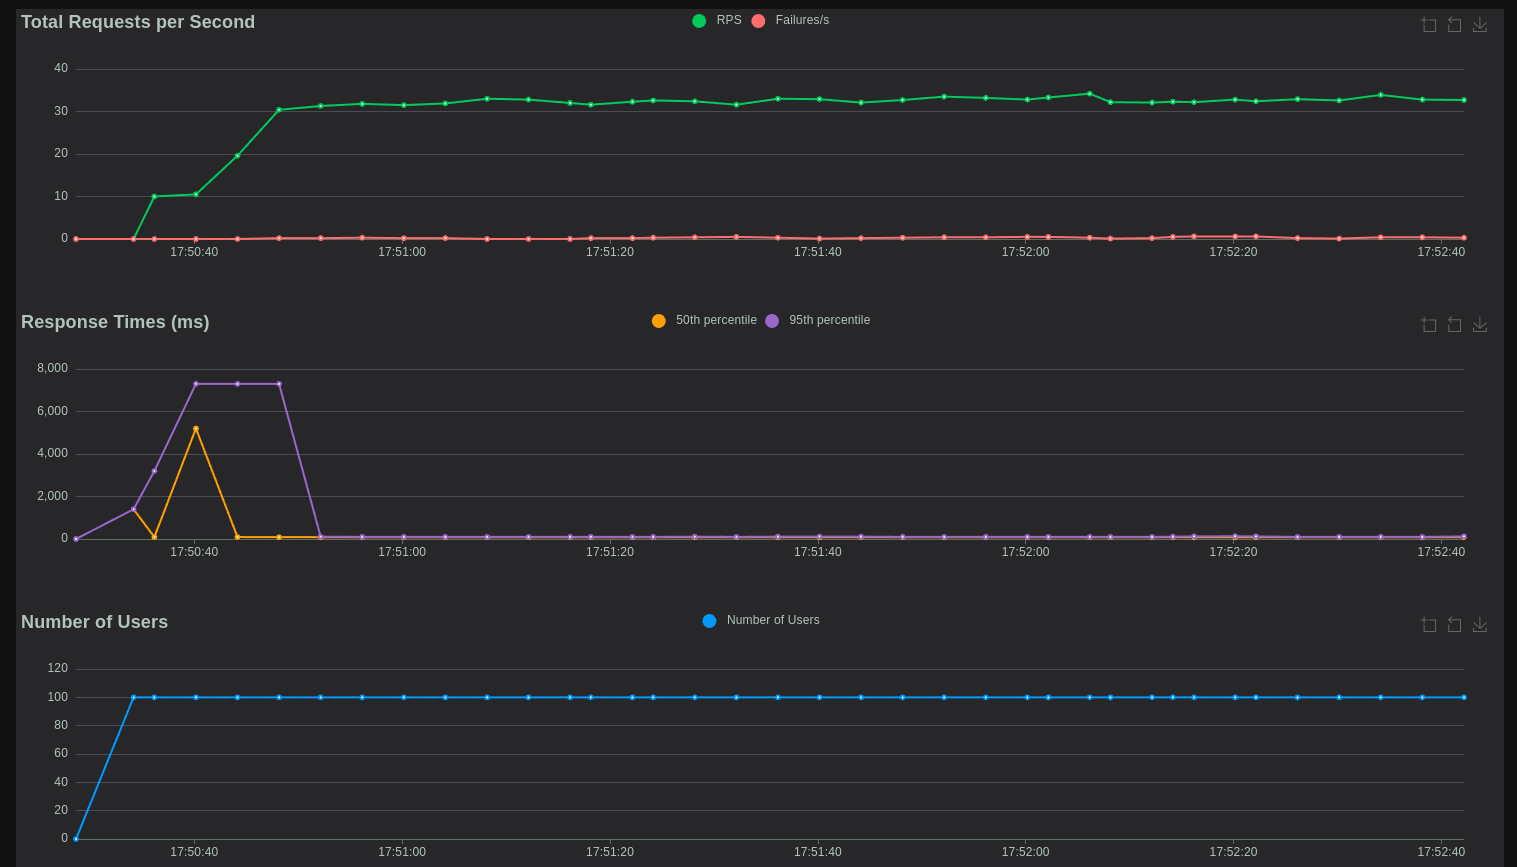
\includegraphics[width=0.9\textwidth]{figures/08_100_1.png}
\caption{Gráfica de la prueba de carga con 100 usuarios concurrentes.}
\label{fig:locust100}
\end{figure}

Se ha observado en la gráfica de ``Response Times (ms)'' un pico inicial de latencia significativa. Aproximadamente entre las 17:30:00 y 17:40:00, el percentil 95 alcanzó hasta 7300 ms (7 segundos) y el percentil 50 (mediana) llegó a unos 5200 ms (5 segundos). Posteriormente, los tiempos de respuesta se estabilizaron rápidamente, lo que es consistente con las estadísticas globales de la prueba, que muestran una mediana de 84 ms y un percentil 95 de 120 ms para el total de la ejecución.
\newline\newline
Este comportamiento es típico de un ``arranque en frío'' o ``cold start'' del sistema, que puede involucrar varios factores:

\begin{itemize}
    \item \textbf{Carga inicial de código:} Al inicio de la prueba, el servidor de aplicaciones necesita cargar el código en memoria, inicializar módulos, frameworks y establecer las primeras conexiones a la base de datos. Este proceso inicial consume tiempo.
    \item \textbf{Calentamiento de cachés:} Las aplicaciones web y las bases de datos (PostgreSQL) utilizan cachés. En las primeras solicitudes, estas cachés están vacías, y los datos deben ser recuperados de fuentes más lentas (disco o base de datos), lo que aumenta la latencia. Conforme más solicitudes llegan, las cachés se llenan, mejorando los tiempos de respuesta.
    \item \textbf{Pool de conexiones:} La creación y llenado del pool de conexiones a la base de datos es una operación relativamente costosa que ocurre al inicio.
    \item \textbf{Menor concurrencia inicial:} A pesar de un rápido incremento a 100 usuarios en la gráfica, las primeras solicitudes pueden impactar un sistema que aún no ha alcanzado su estado ``caliente''.
\end{itemize}
En resumen, estos picos iniciales son un comportamiento esperado de ``calentamiento'' del sistema. Una vez que las cachés se llenan y las conexiones se establecen, el sistema opera de manera más eficiente, resultando en tiempos de respuesta significativamente menores.
\newline\newline
En cuanto a los fallos registrados, una tasa de 35 fallos sobre un total de 4172 solicitudes es **extremadamente baja**, representando una tasa de éxito del 99.20\%. Esto se considera, en la mayoría de los casos, despreciable y no indicativo de un problema sistémico grave. Las posibles causas para estos fallos aislados incluyen:

\begin{itemize}
    \item \textbf{Fallos de red transitorios:} Problemas momentáneos en la conectividad entre el generador de carga y el servidor, o entre el servidor y la base de datos.
    \item \textbf{Timeouts:} Es posible que algunas solicitudes excedieran el tiempo máximo de espera configurado, especialmente durante el período de ``cold start'' donde las latencias eran muy altas.
    \item \textbf{Problemas puntuales del servidor/base de datos:} Eventos raros y breves como micro-reinicios, reinicios de conexión o mantenimiento puntual que afectaron solo a esas solicitudes.
    \item \textbf{Errores del generador de carga:} En ocasiones, el propio software de pruebas puede reportar fallos incorrectamente debido a problemas internos.
\end{itemize}
Dado el bajo número de fallos, no se justifica una investigación profunda sobre su origen, ya que es probable que sean anomalías aleatorias o efectos del proceso de inicialización del sistema. La estadística ``Current Failures/s: 0.5'' indica la tasa de fallos en un momento específico, no contradiciendo el total de fallos de la prueba.
\newline\newline
Además el fallo registrado es en todos los casos el mismo, ``RemoteDisconnected('Remote end closed connection without response')'', lo que indica que el servidor cerró la conexión antes de enviar una respuesta. Esto puede deberse a un timeout o a un cierre inesperado de la conexión por parte del servidor, pero no necesariamente indica un problema grave en el sistema.
\newline\newline
En resumen, los resultados de la prueba de carga con 100 usuarios concurrentes muestran que el sistema es capaz de manejar una carga moderada de usuarios sin problemas significativos, con tiempos de respuesta aceptables y una tasa de éxito muy alta.

\subsubsection{Pruebas de carga con 500 usuarios concurrentes}

En esta prueba se simularon 500 usuarios concurrentes realizando solicitudes al sistema durante 2 minutos. Los resultados obtenidos fueron los siguientes:

\begin{table}[H]
\centering
\resizebox{16cm}{!}{
\begin{tabular}{|r|r|r|r|r|r|r|r|r|r|r|}
\hline
\textbf{Req.} & \textbf{Fails} & \textbf{Med(ms)} & \textbf{95\%(ms)} & \textbf{99\%(ms)} & \textbf{Avg(ms)} & \textbf{Min(ms)} & \textbf{Max(ms)} & \textbf{Avg size(Bytes)} & \textbf{RPS} & \textbf{Fails/s} \\
\hline
4918 & 48 & 88 & 280 & 15000 & 887.77 & 1 & 105514 & 9623.15 & 48.2 & 0.3 \\
\hline
\end{tabular}
}
\caption{Resultados de la prueba de carga con 500 usuarios concurrentes.}
\label{tab:locust500}
\end{table}

\begin{figure}[H]
\centering
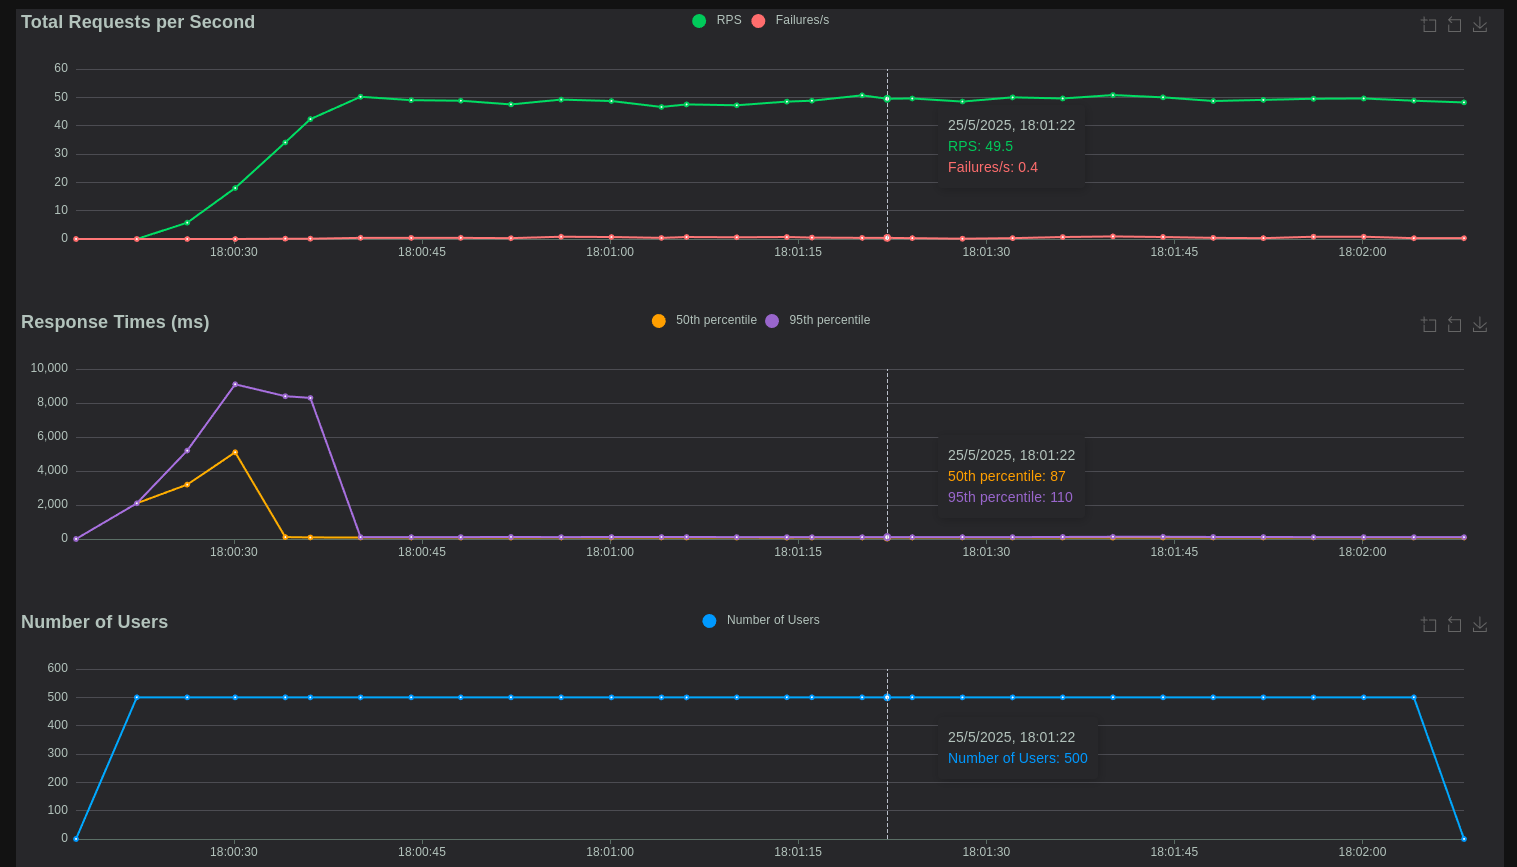
\includegraphics[width=0.9\textwidth]{figures/08_500_1.png}
\caption{Gráfica de la prueba de carga con 500 usuarios concurrentes.}
\label{fig:locust500}
\end{figure}

En esta prueba se observan comporetamientos similares a los de la prueba con 100 usuarios concurrentes, pero con una latencia más alta en general. Esto es esperado, ya que al aumentar el número de usuarios concurrentes, el sistema debe manejar más solicitudes al mismo tiempo, lo que puede aumentar la latencia.
\newline\newline
En la gráfica de ``Response Times (ms)'' se observa un pico de latencia significativa al inicio de la prueba, similar al de la prueba con 100 usuarios concurrentes. En este caso, el percentil 95 alcanzó hasta 9100 ms (9 segundos) y el percentil 50 (mediana) llegó a unos 5100 ms (5 segundos). Posteriormente, los tiempos de respuesta se estabilizaron, lo que es consistente con las estadísticas globales de la prueba, que muestran una mediana de 88 ms y un percentil 95 de 280 ms para el total de la ejecución.
\newline\newline
Además en cuanto a los fallos registrados, una tasa de 48 fallos sobre un total de 4918 solicitudes es también muy baja, representando una tasa de éxito del 99.02\%. Esto indica que el sistema es capaz de manejar una carga moderada de usuarios sin problemas significativos, con tiempos de respuesta aceptables y una tasa de éxito muy alta.
\newline\newline
En resumen, los resultados de la prueba de carga con 500 usuarios concurrentes muestran que el sistema es capaz de manejar una carga moderada de usuarios sin problemas significativos, con tiempos de respuesta aceptables y una tasa de éxito muy alta. Aunque se observan picos de latencia al inicio de la prueba, estos son esperados y no indican un problema grave en el sistema.

\subsubsection{Pruebas de carga con 1000 usuarios concurrentes}

En esta prueba se simularon 1000 usuarios concurrentes realizando solicitudes al sistema durante 2 minutos. Los resultados obtenidos fueron los siguientes:

\begin{table}[H]
\centering
\resizebox{16cm}{!}{
\begin{tabular}{|r|r|r|r|r|r|r|r|r|r|r|}
\hline
\textbf{Req.} & \textbf{Fails} & \textbf{Med(ms)} & \textbf{95\%(ms)} & \textbf{99\%(ms)} & \textbf{Avg(ms)} & \textbf{Min(ms)} & \textbf{Max(ms)} & \textbf{Avg size(Bytes)} & \textbf{RPS} & \textbf{Fails/s} \\
\hline
6672 & 215 & 92 & 2500 & 89000 & 2829.37 & 5 & 135196 & 9404.85 & 50.1 & 0.6 \\
\hline
\end{tabular}
}
\caption{Resultados de la prueba de carga con 1000 usuarios concurrentes.}
\label{tab:locust1000}
\end{table}

\begin{figure}[H]
\centering
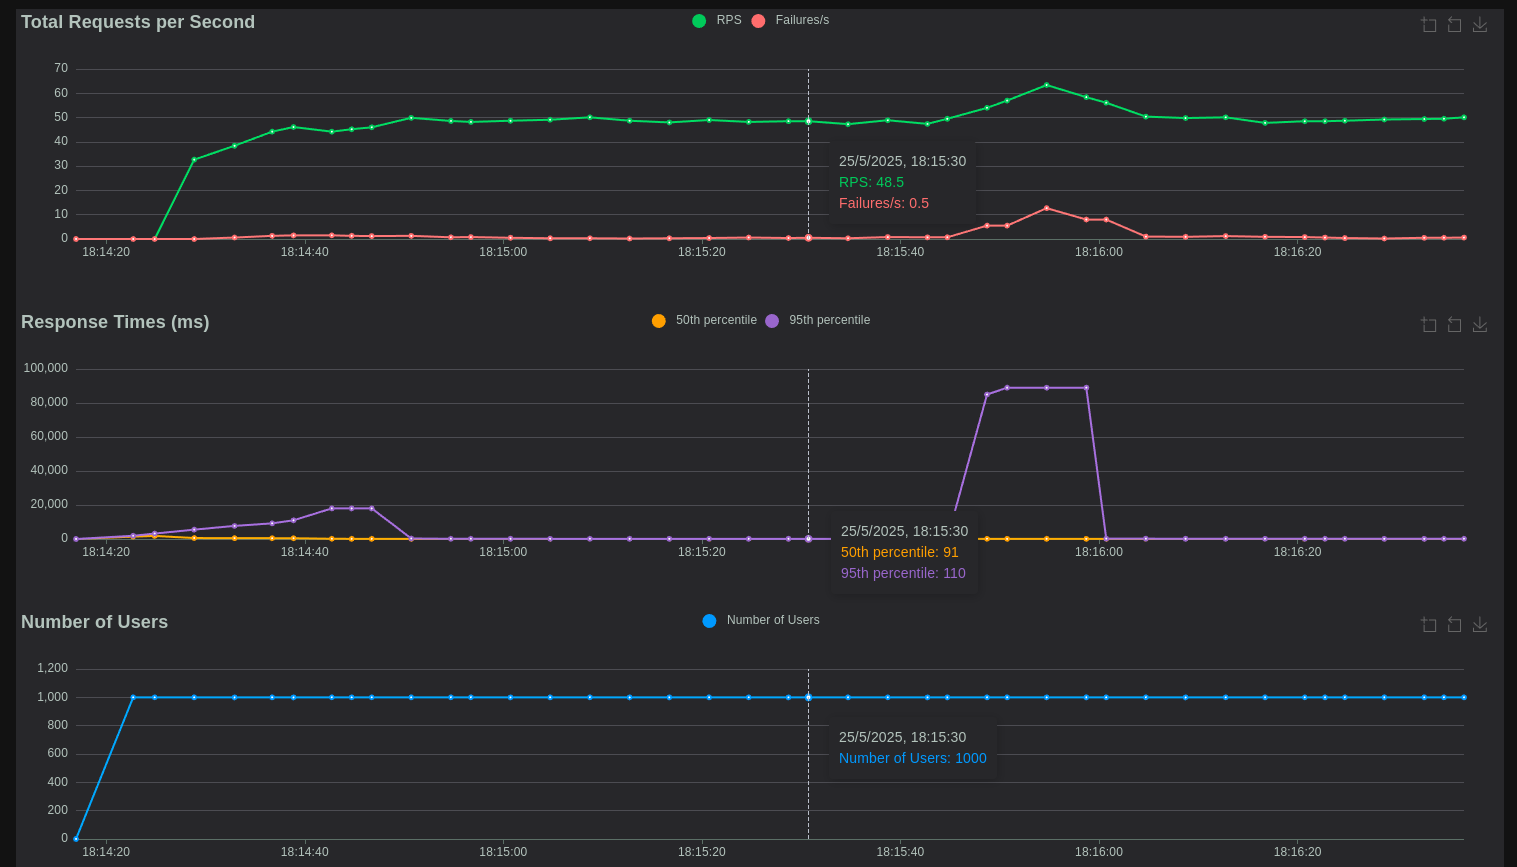
\includegraphics[width=0.9\textwidth]{figures/08_1000_1.png}
\caption{Gráfica de la prueba de carga con 1000 usuarios concurrentes.}
\label{fig:locust1000}
\end{figure}

En este caso se observa un comportamiento similar al de las pruebas anteriores, pero con una latencia aún más alta en general. Esto es esperado, ya que al aumentar el número de usuarios concurrentes, el sistema debe manejar más solicitudes al mismo tiempo, lo que puede aumentar la latencia.
\newline\newline
En la gráfica de ``Response Times (ms)'' se observa un pico de latencia significativa al inicio de la prueba, similar al de las pruebas anteriores. En este caso, el percentil 95 alcanzó hasta 18000 ms (18 segundos) y el percentil 50 (mediana) sin embargo no es tan alto como el de las otras pruebas, llegando a un pico de 140ms al principio. Posteriormente, los tiempos de respuesta se estabilizaron, lo que es consistente con las estadísticas globales de la prueba, que muestran una mediana de 92 ms y un percentil 95 de 2500 ms para el total de la ejecución.
\newline\newline
Además, en cuanto a los fallos registrados, una tasa de 215 fallos sobre un total de 6672 solicitudes es también baja, representando una tasa de éxito del 96.78\%. Aunque esta tasa es inferior a las pruebas anteriores, sigue siendo aceptable y no indica un problema grave en el sistema.
\newline\newline
En esta prueba además se ha observado un comportamiento anómalo alrededor de los 90 segundos de la prueba, donde el percentil 99 alcanzó hasta 89000 ms (89 segundos). Esto indica que hubo un problema puntual en el sistema que afectó a algunas solicitudes, pero no a todas. Este tipo de comportamiento puede deberse a un problema de rendimiento en el servidor o en la base de datos, o a un problema de red.

La ``recuperación'' no se observa en el sentido de que los tiempos de respuesta o fallos vuelvan a niveles óptimos durante esta fase. Más bien, el sistema entra en un estado de alta latencia y fallos continuos bajo esta carga sostenida. La estabilización en el gráfico de tiempos de respuesta a partir de los 80 segundos no es una recuperación positiva, sino una indicación de que el sistema se ha atascado en un estado de rendimiento muy bajo.
\newline
Las causas de esta saturación con 1000 usuarios concurrentes pueden ser:

\begin{itemize}
    \item \textbf{Saturación de recursos del servidor:} Límites de CPU, memoria o procesos en el servicio de aplicación.
    \item \textbf{Cuellos de botella en la base de datos:} Agotamiento del pool de conexiones, contención de bloqueos, o límites de recursos (CPU, RAM, IOPS) en PostgreSQL.
    \item \textbf{Timeouts:} Los tiempos de respuesta excesivos probablemente provocan que las solicitudes excedan los límites de tiempo establecidos, registrándose como fallos.
    \item \textbf{Límites de autoescalado:} Si el autoescalado no es suficientemente rápido o los límites del plan de servicio son insuficientes para 1000 usuarios.
\end{itemize}
    
    \chapter{Conclusiones y trabajos futuros}\label{cap:conclusiones}

\Juanmi[]{Punto a revisar}

El sistema completo, ``TempusUGR'', ha sido desarrollado y desplegado con éxito. Además de estar preparado para un uso normal, se han implementado varias características que lo hacen un sistema robusto y escalable. 

\section{Objetivos cumplidos}
Todos los objetivos planteados al inicio del proyecto se han cumplido, aunque algunos de ellos han evolucionado a lo largo del desarrollo. En particular, se ha logrado:
\begin{itemize}
    \item Desarrollar un sistema de gestión de horarios para la Universidad de Granada que permita a los estudiantes y profesores visualizar sus horarios de manera eficiente.
    \item Proveer al usuario un archivo ``ical'' que pueda ser importado en aplicaciones de calendario como Google Calendar, Apple Calendar, Outlook, etc.
    \item Permitir la sincronización de los horarios con aplicaciones de calendario, facilitando la gestión del tiempo y la planificación de actividades académicas.
    \item Agilizar el proceso de comunicaciones de eventos tanto de grupo como de facultades, a nivel de la UGR.
    \item Implementar una interfaz de usuario intuitiva y fácil de usar, que permita a los usuarios interactuar con el sistema de manera eficiente.
    \item Aprender sobre la arquitectura de microservicios, y sobre varias tecnologías relativas a este tipo de arquitectura.
    \item Desplegar el sistema en un entorno de producción, utilizando herramientas de contenedorización y orquestación como Docker y Docker Compose.
\end{itemize}

\section{Dificultades y resolución}

El proyecto ha supuesto un reto significativo tanto a nivel técnico como a nivel de gestión. Algunas de las dificultades encontradas incluyen:
\begin{itemize}
    \item El sistema se planteó inicialmente como un apoyo a las sedes de la UGR para la subida de información de horarios a una única plataforma de manera estándar. Tras la primera entrevista con Jesús García Miranda, Secretario de la ETSIIT y encargado de la gestión de horarios, se decidió cambiar de dirección hacia un sistema que utilizara los datos ya publicados en un punto central (en este caso Grados UGR).
    Esta decisión se tomó por la falta de información en cuanto a la generación, formato y fechas relativas a la subida de horarios, así como por la falta de un sistema centralizado que permitiera a las sedes subir sus horarios de manera estandarizada.
    Sin embargo, esta decisión también ha permitido centrar el proyecto en una solución más escalable y flexible, que puede adaptarse a futuras necesidades de la UGR.

    \item Desde un principio se plantearon varias opciones para la implementación del sistema. Desde solicitar una vista o API a la base de datos de los horarios y calendario académico, desde integrar el sistema de autenticación institucional u obtener la información relativa a las matriculaciones. Al no poder tener acceso a ninguna de estas opciones, se optó por soluciones alternativas e ``independientes'' de la UGR, como la utilización de los datos publicados en Grados UGR y la implementación de un sistema de autenticación propio.
    \item Aunque se realizaron varias reuniones con el director del TFG, Juan Luis Jiménez Laredo, para concretar el alcance y requisitos del proyecto, es inevitable que con la evolución de este se hayan presentado nuevos casos de uso y funcionalidades que no estaban contemplados inicialmente. Esto ha requerido una adaptación constante del proyecto, que gracias a la metodología ágil utilizada, se ha podido gestionar de manera eficiente.
\end{itemize}

Todo el desarrollo del sistema (repositorios del backend, frontend, despliegue y documentación) se puede consultar de manera centralizada en la organización de GitHub [\href{https://github.com/TempusUGR}{TempusUGR}]. De este modo se facilita la colaboración y el mantenimiento del proyecto, permitiendo que otros desarrolladores puedan contribuir y mejorar el sistema en el futuro.
Además se puede visualizar también a través de su propio ``Github Project'' [\href{https://github.com/orgs/TempusUGR/projects/3}{TempusUGR Project}] tanto los tableros de tareas, issues y pull requests del proyecto, como el ``roadmap'' con la temporización real de las tareas y funcionalidades implementadas.

\section{Mejoras posibles y trabajos futuros}

Aunque el sistema ha sido desarrollado y desplegado con éxito, siempre hay margen para mejoras y nuevas funcionalidades. Algunas de las posibles mejoras y trabajos futuros incluyen:
\begin{itemize}
    \item Integración con otros sistemas institucionales de la UGR, como la API de los horarios, autenticación institucional, matriculaciones, etc. Esto permitiría una mayor interoperabilidad y una mejor experiencia de usuario.
    Además la posibilidad de integrar TempusUGR con plataformas establecidas como Prado UGR o SWAD , podría facilitar la adopción del sistema por parte de los usuarios y mejorar la experiencia general.
    \item Implementación de un sistema de notificaciones para alertar a los usuarios sobre cambios en sus horarios de clases oficiales.
    \item Optimización del rendimiento del sistema para manejar un mayor volumen de usuarios y datos, asegurando que el sistema sea escalable y eficiente.
    \item Implementación  de monitorización y estadísticas para analizar el uso del sistema y detectar posibles problemas o áreas de mejora.
    \item Integrar sistemas de Integración Continua/Despliegue Continuo (CI/CD) para facilitar el desarrollo y despliegue de nuevas funcionalidades, asegurando que el sistema se mantenga actualizado y libre de errores. Esto permitiría también una mayor colaboración entre los desarrolladores y una mejor gestión del código fuente.
\end{itemize}

    
    % Ensure all environments are properly closed
    % Check for unclosed \begin{enumerate} in included files.
    
    % Bibliografía
    \bibliographystyle{unsrtnat}
    \bibliography{bibliografia.bib}

    % Anexos

    %% Anexo : Glosario 
    \chapter*{Anexo: Glosario}
\addcontentsline{toc}{chapter}{Anexo: Glosario}

A continuación se presenta un glosario con las definiciones de términos técnicos utilizados a lo largo del trabajo:

\begin{description}
    \item [\hypertarget{scrum}{SCRUM}]: es un marco de trabajo ágil para el desarrollo de software. Se basa en la iteración y la colaboración entre los miembros del equipo de desarrollo.
    \item [\hypertarget{backlog}{Backlog}]: es una lista priorizada de tareas y requisitos que deben completarse en un proyecto. El backlog se utiliza para planificar el trabajo en cada sprint.
    \item [\hypertarget{lms}{LMS}]: es un sistema de gestión de aprendizaje. Se utiliza para administrar, documentar, rastrear, informar y entregar cursos de formación. Un ejemplo de LMS es Moodle, que es un sistema de gestión de aprendizaje de código abierto.
    \item [\hypertarget{docker}{Docker}]: es una plataforma de software que permite crear, desplegar y ejecutar aplicaciones en contenedores. Los contenedores son entornos ligeros y portátiles que permiten ejecutar aplicaciones de manera aislada del sistema operativo subyacente.
    \item [\hypertarget{microservicios}{Microservicios}]: es un estilo arquitectónico que estructura una aplicación como un conjunto de servicios pequeños y autónomos. Cada servicio se ejecuta en su propio proceso y se comunica con otros servicios a través de APIs.
    \item [\hypertarget{api}{API}]: es un conjunto de definiciones y protocolos que permiten la comunicación entre diferentes sistemas. Las APIs permiten que diferentes aplicaciones se comuniquen entre sí y compartan datos.
    \item [\hypertarget{backend}{Backend}]: es la parte de una aplicación que se encarga de la lógica de negocio y el acceso a los datos. El backend se ejecuta en un servidor y se comunica con el frontend a través de APIs.
    \item [\hypertarget{frontend}{Frontend}]: es la parte de una aplicación que se encarga de la interfaz de usuario y la interacción con el usuario. El frontend se ejecuta en el navegador del usuario y se comunica con el backend a través de APIs.
    \item [\hypertarget{ssl}{SSL}]: es un protocolo de seguridad que se utiliza para establecer una conexión segura entre un servidor y un cliente. SSL cifra los datos que se envían entre el servidor y el cliente, lo que protege la información sensible de ser interceptada por terceros.
    \item [\hypertarget{https}{HTTPS}]: es una versión segura de HTTP. HTTPS utiliza SSL para cifrar los datos que se envían entre el servidor y el cliente, lo que protege la información sensible de ser interceptada por terceros.
    \item [\hypertarget{ui}{UI}]: es la interfaz de usuario. Se refiere a la parte de una aplicación con la que el usuario interactúa. La UI incluye elementos como botones, menús y formularios.
    \item [\hypertarget{ux}{UX}]: es la experiencia del usuario. Se refiere a la forma en que un usuario interactúa con una aplicación y cómo se siente al hacerlo. La UX incluye aspectos como la usabilidad, la accesibilidad y la satisfacción del usuario.
    \item [\hypertarget{jwt}{JWT}]: es un estándar abierto que define un formato compacto y autónomo para transmitir información de forma segura entre partes como un objeto JSON. Esta información puede ser verificada y confiable porque está firmada digitalmente.
    \item [\hypertarget{sso}{SSO}]: es un proceso de autenticación que permite a un usuario acceder a múltiples aplicaciones con una sola sesión de inicio de sesión. SSO simplifica la gestión de credenciales y mejora la experiencia del usuario al reducir la necesidad de recordar múltiples contraseñas.
    \item [\hypertarget{rest}{REST}]: es un estilo arquitectónico para diseñar servicios web. REST se basa en el uso de HTTP y utiliza los métodos HTTP (GET, POST, PUT, DELETE) para realizar operaciones sobre recursos.
    \item [\hypertarget{graphql}{GraphQL}]: es un lenguaje de consulta para APIs y un entorno de ejecución para ejecutar esas consultas con los datos existentes. GraphQL permite a los clientes solicitar solo los datos que necesitan, lo que reduce la cantidad de datos transferidos entre el cliente y el servidor.
    \item [\hypertarget{grpc}{gRPC}]: es un marco de trabajo de código abierto que permite la comunicación entre aplicaciones distribuidas. gRPC utiliza HTTP/2 para la comunicación y Protocol Buffers como formato de serialización de datos.
    \item [\hypertarget{reverseproxy}{Reverse Proxy}]: es un servidor que actúa como intermediario entre los clientes y uno o más servidores de backend. El reverse proxy recibe las solicitudes de los clientes y las reenvía a los servidores de backend, lo que permite distribuir la carga y mejorar la seguridad.
    \item [\hypertarget{cronjob}{Cron Job}]: es una tarea programada que se ejecuta automáticamente en un servidor en intervalos regulares. Los cron jobs se utilizan para realizar tareas de mantenimiento, como copias de seguridad, limpieza de registros y actualizaciones de datos.
\end{description}

\endinput
        

% Fin del documento
\end{document}
